% ****************************************************************************************** % Dissertation template and document class for Princeton University
% Author  : Jeffrey Scott Dwoskin <jdwoskin@princeton.edu>
% Adapted from: http://www.math.princeton.edu/graduate/tex/puthesis.html
% ****************************************************************************************** %


%%% For print copies
%% set 'singlespace' option to set entire thesis to single space, and define "\printmode" to remove all hyperlinks for printed copies of the thesis. Delete all output files before changing this mode -- it will turn hyperref package on and off
%\documentclass[12pt,lot, lof, singlespace]{puthesis}
%\newcommand{\printmode}{}

%%% For the electronic copy, use doublespacing, define "\proquestmode" to use outlined links, instead of colored links. 
\documentclass[12pt,lot, lof]{puthesis}
\newcommand{\proquestmode}{}
% I prefer proquestmode to be off for electronic copies for normal use, since the colored links are less distracting. However when printed in black and white, the colored links are difficult to read. 

%%% For early drafts without some of the frontmatter
% Also see the "ifodd" command below to disable more frontmatter
%\documentclass[12pt]{puthesis}

%%%%%%%%%%%%%%%%%%%%%%%%%%%%%%%%%%%%%%%%%%%%%%%%%%%%%%%%%%%%%\
%%%% Author & title page info

\title{Search for Double Higgs Production in the Final State with Two Photons and Two Bottom Quarks
with the CMS Detector}

\submitted{September 2015}  % degree conferral date (January, April, June, September, or November)
\copyrightyear{2015}  % year in which the copyright is secured by publication of the dissertation.
\author{Philip Robert Hebda}
\adviser{Daniel Robert Marlow}  %replace with the full name of your adviser
%\departmentprefix{Program in}  % defaults to "Department of", but programs need to change this.
\department{Physics}

%%%%%%%%%%%%%%%%%%%%%%%%%%%%%%%%%%%%%%%%%%%%%%%%%%%%%%%%%%%%%\
%%%% Tweak float placements
% From: http://mintaka.sdsu.edu/GF/bibliog/latex/floats.html "Controlling LaTeX Floats"
% and based on: http://www.tex.ac.uk/cgi-bin/texfaq2html?label=floats
% LaTeX defaults listed at: http://people.cs.uu.nl/piet/floats/node1.html

% Alter some LaTeX defaults for better treatment of figures:
    % See p.105 of "TeX Unbound" for suggested values.
    % See pp. 199-200 of Lamport's "LaTeX" book for details.
    %   General parameters, for ALL pages:
    \renewcommand{\topfraction}{0.85}	% max fraction of floats at top
    \renewcommand{\bottomfraction}{0.6}	% max fraction of floats at bottom
    %   Parameters for TEXT pages (not float pages):
    \setcounter{topnumber}{2}
    \setcounter{bottomnumber}{2}
    \setcounter{totalnumber}{4}     % 2 may work better
    \setcounter{dbltopnumber}{2}    % for 2-column pages
    \renewcommand{\dbltopfraction}{0.66}	% fit big float above 2-col. text
    \renewcommand{\textfraction}{0.15}	% allow minimal text w. figs
    %   Parameters for FLOAT pages (not text pages):
    \renewcommand{\floatpagefraction}{0.66}	% require fuller float pages
	% N.B.: floatpagefraction MUST be less than topfraction !!
    \renewcommand{\dblfloatpagefraction}{0.66}	% require fuller float pages

% The documentclass already sets parameters to make a high penalty for widows and orphans. 

%%%%%%%%%%%%%%%%%%%%%%%%%%%%%%%%%%%%%%%%%%%%%%%%%%%%%%%%%%%%%\
%%%% Use packages

%\usepackage{amsfonts}
\usepackage{amsmath}

%%% For figures
\usepackage{graphicx}
%\usepackage{subfig,rotate}
\usepackage{float}

%%% for comments
\usepackage{verbatim}

%%% For tables
\usepackage{multirow}
% Longtable lets you have tables that span multiple pages.
\usepackage{longtable}

% Booktabs produces far nicer tables than the standard LaTeX tables.
%   see: http://en.wikibooks.org/wiki/LaTeX/Tables
\usepackage{booktabs}

%set parameters for longtable:
% default caption width is 4in for longtable, but wider for normal tables
\setlength{\LTcapwidth}{\textwidth}



%%%%%%%%%%%%%%%%%%%%%%%%%%%%%%%%%%%%%%%%%%%%%%%%%%%%%%%%%%
%%% Printed vs. online formatting
\ifdefined\printmode

% Printed copy
% url package understands urls (with proper line-breaks) without hyperlinking them
\usepackage{url}


\else

\ifdefined\proquestmode
%ProQuest copy -- http://www.princeton.edu/~mudd/thesis/Submissionguide.pdf

% ProQuest requires a double spaced version (set previously). They will take an electronic copy, so we want links in the pdf, but also copies may be printed or made into microfilm in black and white, so we want outlined links instead of colored links.
\usepackage{hyperref}
\hypersetup{bookmarksnumbered}

% copy the already-set title and author to use in the pdf properties
\makeatletter
\hypersetup{pdftitle=\@title,pdfauthor=\@author}
\makeatother

\else
% Online copy

% adds internal linked references, pdf bookmarks, etc

% turn all references and citations into hyperlinks:
%  -- not for printed copies
% -- automatically includes url package
% options:
%   colorlinks makes links by coloring the text instead of putting a rectangle around the text.
\usepackage{hyperref}
\hypersetup{colorlinks,bookmarksnumbered}

% copy the already-set title and author to use in the pdf properties
\makeatletter
\hypersetup{pdftitle=\@title,pdfauthor=\@author}
\makeatother

% make the page number rather than the text be the link for ToC entries
%\hypersetup{linktocpage}
\fi % proquest or online formatting
\fi % printed or online formatting


%%%%%%%%%%%%%%%%%%%%%%%%%%%%%%%%%%%%%%%%%%%%%%%%%%%%%%%%%%%%%\
%%%% Define commands

% Define any custom commands that you want to use.
% For example, highlight notes for future edits to the thesis
%\newcommand{\todo}[1]{\textbf{\emph{TODO:}#1}}


% create an environment that will indent text
% see: http://latex.computersci.org/Reference/ListEnvironments
% 	\raggedright makes them left aligned instead of justified
\newenvironment{indenttext}{
    \begin{list}{}{ \itemsep 0in \itemindent 0in
    \labelsep 0in \labelwidth 0in
    \listparindent 0in
    \topsep 0in \partopsep 0in \parskip 0in \parsep 0in
    \leftmargin 1em \rightmargin 0in
    \raggedright
    }
    \item
  }
  {\end{list}}

% another environment that's an indented list, with no spaces between items -- if we want multiple items/lines. Useful in tables. Use \item inside the environment.
% 	\raggedright makes them left aligned instead of justified
\newenvironment{indentlist}{
    \begin{list}{}{ \itemsep 0in \itemindent 0in
    \labelsep 0in \labelwidth 0in
    \listparindent 0in
    \topsep 0in \partopsep 0in \parskip 0in \parsep 0in
    \leftmargin 1em \rightmargin 0in
    \raggedright
    }

  }
  {\end{list}}



%%%%%%%%%%%%%%%%%%%%%%%%%%%%%%%%%%%%%%%%%%%%%%%%%%%%%%%%%%%%%\
%%%% Front-matter

% For early drafts, you may want to disable some of the frontmatter. Simply change this to "\ifodd 1" to do so.
\ifodd 0
% front-matter disabled while writing chapters
\renewcommand{\maketitlepage}{}
\renewcommand*{\makecopyrightpage}{}
\renewcommand*{\makeabstract}{}

% you can just skip the \acknowledgements and \dedication commands to leave out these sections.

\else


\abstract{
% Abstract can be any length, but should be max 350 words for a Dissertation for ProQuest's print indicies (150 words for a Master's Thesis) or it will be truncated for those uses.
This is a \LaTeX{} template and document class for Ph.D. dissertations at Princeton University. It was created in 2010 by Jeffrey Dwoskin, and adapted from a template provided by the math department. Their original version is available at: \url{http://www.math.princeton.edu/graduate/tex/puthesis.html}

This is \textbf{NOT} an official document. Please verify the current Mudd Library dissertation requirements~\cite{mudd2009} and any department-specific requirements before using this template or document class.


Your abstract can be any length, but should be a maximum of 350 words for a Dissertation for ProQuest's print indicies (or 150 words for a Master's Thesis); otherwise it will be truncated for those uses~\cite{proquest2006}.


Dwoskin Ph.D. Dissertation Template --- version 1.0, 5/19/2010
}

\acknowledgements{
%I would like to thank...
in progress

This thesis would not have been possible without the input of many.
First, I would like to thank my advisor Dan Marlow, who has guided me through five years of
graduate study. I have enjoyed and profited from our conversations related
to all things physics and, occasionally, to life. I have seen that doing research at times involves
more than doing physics, and Dan's advice in navigating the bureaucracies created by
CMS and the Graduate School has been refreshingly helpful.

I would like to thank the professors in the Princeton Physics Department, in particular to Chris Tully
for discussions related to this thesis and for reading this thesis and to Igor Klebanov
and Peter Meyers for serving on committees for my FPO and pre-thesis project.

From my time at Purdue as an undergraduate, I would like to thank my advisor Daniela Bortoletto and
Artur Apresyan. Through our work at CDF, their influence and patience gave me strong desire to
see just how deep the rabbit hole goes (through graduate study).
%particle physics was an interesting and worthwhile endeavor.

At CERN, I have had the priveledge to work with many talented physicists. In the HggHbb group,
through which the main result of this thesis was achieved, I have had the pleasure to collaborate with
Olivier Bondu, Maxime Gouzevitch, Chiara Rovelli, Badder Marzocchi, Alexandra Oliveira, and
Amina Zghiche. I would especially like to thank Olivier for forcing the use of GitHub in our group,
ultimately making collabration easier and more enjoyable.

I owe thanks to many others with whom I have collaborated on other CMS projects.
Of the 4000 authors that comprise the CMS author list, I would like to single out the following
who have contributed in some way to my time at CMS:
from the luminosity subsystem Nadia Adam, Andrzej Zuranski, Adam Hunt, and Paul Lujan;
from the Pixel Luminosity Telescope Dean Hidas, Steve Schnetzer, Bob Stone, Andreas Kornmayer, and Andres Delannoy;
from the $W'$ analysis Christos Leonidopoulos and Sunghyun Chang;
from the $VH(b\bar{b})$ analysis Seth Zenz and Michael Mooney.

I would like to thank the friends over the years who have made life as, or sometimes more, interesting
than my physics life. These include, in some nonrandom order,
<people> cern, princeton, 400
I would also like to thank Tuna, Kurt, Josh, and Josh for contributing to multiple versions
of our CERN relay team and, in turn, creating a true American dynasty. Heros are forged in the fire.

La langue française occupe un endoit special pendant le temps que j'ai passé comme doctorant.
Au moment que j'ai su que je démenagerais à Genève, j'ai commencé à l'apprendre avec l'aide de
plusieurs personnes patientes à Princeton et à Genève, des amis ainsi que des professeurs.
Je remercie <people> french friends en français (teachers, croix rouge, roberto, emilie).

I would like to thank my family whom I have been very fortunate to have by my side through ups and
downs. To my brothers, through many years of laughing and fighting, 
To my parents, waaa

Finally, to my fiancée Jigisha Darbha, thanks. Your companionship has provided me much opportunity
to grow as a person and has served as a sanity check.
I am excited that we will soon be on the same team. And as always, I ask for your patience
while I slowly learn the language of your ancestors. I look forward to many more adventures
to come.

\\
This thesis has been supported by the NSF Graduate Research Fellowship
and the U.S. Department of Energy.




}

%\dedication{To Dad,\\for practicing spelling words with me\\and driving me 770 miles to and from the GC,
%\\among other things.}
\dedication{make a dedication, in progress}

\fi  % disable frontmatter


%%%%%%%%%%%%%%%%%%%%%%%%%%%%%%%%%%%%%%%%%%%%%%%%%%%%%%%%%%%%%\
%%%% Hide some chapters

%%% If you want to produce a pdf that includes only certain chapters, specify them with includeonly, in addition to including all chapters below.
%\includeonly{ch-intro/chapter-intro}
%%% You can also specify multiple chapters.
%\includeonly{ch-intro/chapter-intro,ch-usage/chapter-usage}
%\includeonly{chap1,chap2,chap3}


%%%%%%%%%%%%%%%%%%%%%%%%%%%%%%%%%%%%%%%%%%%%%%%%%%%%%%%%%%%%%
%%%% Notes:

% Footnotes should be placed after punctuation.\footnote{place here.}
% Generally, place citations before the period~\cite{anotherauthor}.
% The proper usage for i.e., and e.g., include commas ``(e.g., option A, option B)''

%%%%%%%%%%%%%%%%%%%%%%%%%%%%%%%%%%%%%%%%%%%%%%%%%%%%%%%%%%%%%
%%%% Import chapters

\begin{document}

\makefrontmatter


% USER-DEFINED STUFF 
\newcommand{\Hgg}{\ensuremath{H\to\gamma\gamma}}
\newcommand{\Hbb}{\ensuremath{H\to b\bar{b}}}
\newcommand{\ggbb}{\ensuremath{\gamma\gamma b\bar{b}}}
\newcommand{\ggjj}{\ensuremath{\gamma\gamma jj}}
\newcommand{\gjjj}{\ensuremath{\gamma jjj}}
\newcommand{\Mgg}{\ensuremath{m_{\gamma\gamma}}}
\newcommand{\Mjj}{\ensuremath{m_{jj}}}
\newcommand{\Mjjr}{\ensuremath{m_{jj}^{\rm r}}}
\newcommand{\thetastar}{\ensuremath{\theta^{\rm CS}_{HH}}}
\newcommand{\acosthetastar}{\ensuremath{|\cos {\theta^{\rm CS}_{HH}}|}}
\newcommand{\Mggjj}{\ensuremath{m_{\gamma\gamma jj}}}
\newcommand{\Mggjjk}{\ensuremath{m_{\gamma\gamma jj}^{\rm kin}}}
\newcommand{\Mggjjrk}{\ensuremath{m_{\gamma\gamma jj}^{\rm r, kin}}}
\newcommand{\pTj}{\ensuremath{p_{T, j}}}
\newcommand{\pTjr}{\ensuremath{p_{T, j}^r}}
\newcommand{\kapt}{\ensuremath{\kappa_{t}}}
\newcommand{\kapl}{\ensuremath{\kappa_{\lambda}}}
\newcommand{\ctwo}{\ensuremath{c_2}}
\newcommand{\sieie}{\ensuremath{\sigma_{i\eta i\eta}}}
\newcommand{\met}{\ensuremath{{\not\mathrel{E}}_{\text{T}}}}


% If you've disabled frontmatter, you can insert the toc manually
%\tableofcontents\clearpage

% \include lets us split up the document (and each include starts a new page):

\chapter{Introduction\label{ch:intro}}

Our understanding of fundamental particles and interactions has progressed much from the early days.
These beginnings could be with Empdocles and his four roots fire, earth, air, and water, or with
Aristotle relating these four roots to two of the four sensible quantities hot, dry, wet, and
cold~\cite{0415078547} as in Figure~\ref{fig:aristotle}
(not to omit classical elements from other philosophies and worldviews), or more recently with
John Dalton's atoms~\cite{dalton}. Or perhaps particle physics began with
the discovery of the electron by J.J. Thomson in 1897~\cite{thomson:electron},
which to this day has not been observed
to have internal structure or decay, with upper (lower) bounds on the radius (lifetime) of
10$^{-22}$~m (10$^{26}$~years)~\cite{1988PhST...22..102D,2002PhLB..525...29B}.

\begin{figure}[ht]
 \begin{center}
    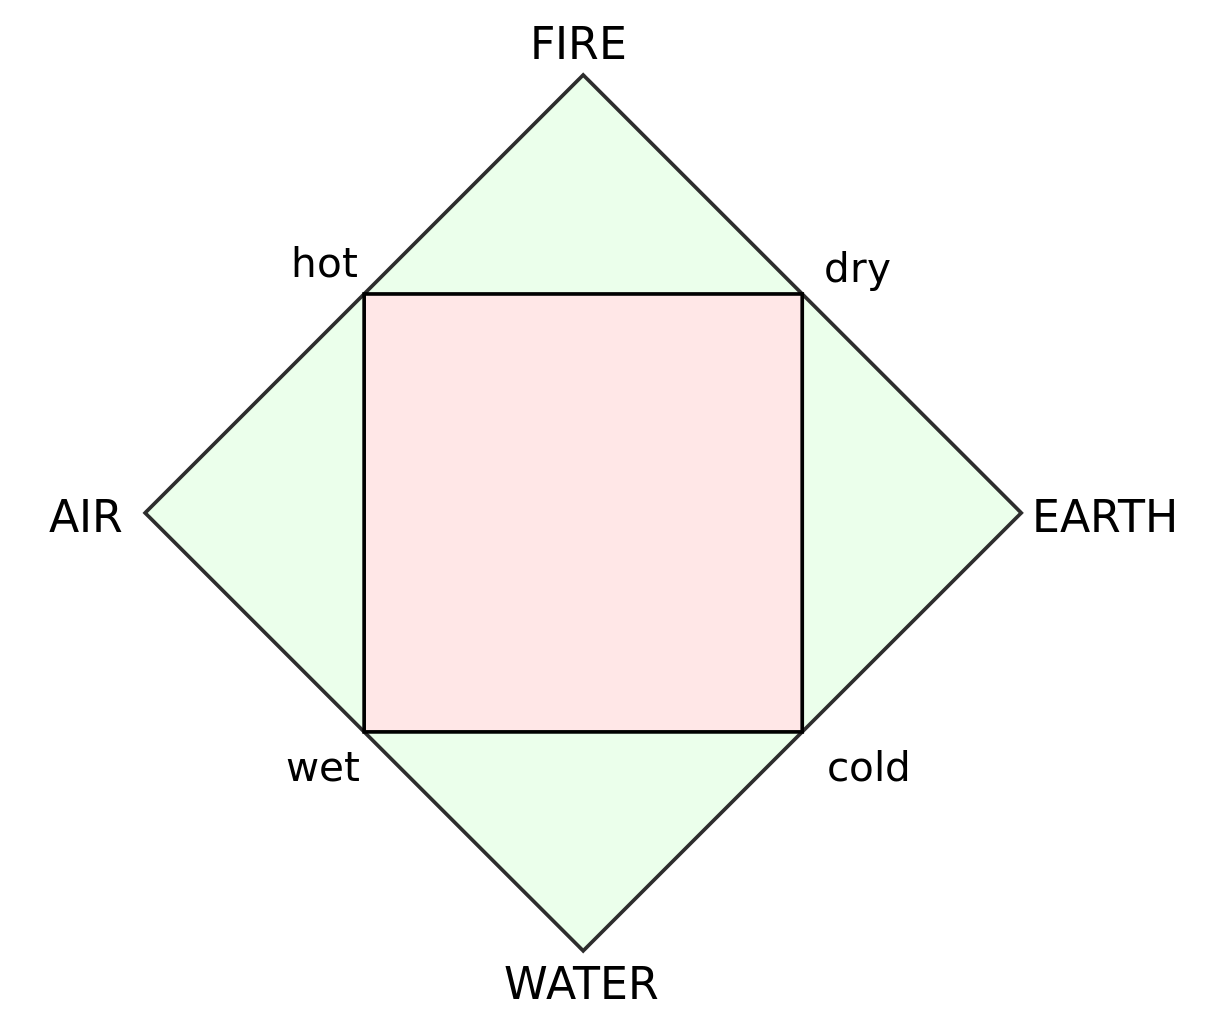
\includegraphics[width=0.90\textwidth]{figures/intro/Four_elements_representation.png}
      \end{center}
\caption{The four roots how they relate to the sensible quantities.}
\label{fig:aristotle}
\end{figure}

Today we have the Standard Model, the theoretical framework that best describes the
experimentally oberserved phenomena of the fundamental particles and their interactions. The theory
is not perfect, and it remains an overarching theme of particle physics to unify physical processes
at all energy scales under one single framework, if such a thing can be done at all.
The SM, its successes, and its shortcomings are described in
Sections~\ref{sec:SM}, \ref{sec:SMsuccess}, and \ref{sec:SMshortcomings}.

Recently in 2012, the last piece to the SM was put into place with the discovery of the Higgs boson.
This discovery, described in Section~\ref{sec:discovery}, is the foundation for the work based on
this thesis, the goal of which is to describe the first search for diHiggs production, a process
in which two Higgs bosons are produced. The motivations for what the search for this process means
in the context of SM physics and ``new'' physics is given in Section~\ref{sec:diHiggs}.

Finally, for those readers who have by chance come across this thesis and do not
have any physics training, Appendix~\ref{ch:mom} may be especially appealing.

\section{The Standard Model\label{sec:SM}}

The Standard Model (SM) of particle physics is a relativistic quantum field theory
that describes how the known fundamental particles interact through the electromagnetic, weak,
and strong forces.
The theory was developed through the unification of the electromagnetic and weak forces by Glashow
in 1961~\cite{1961.Glashow.Partial-symmetries} and through the incorporation of this electroweak
theory with the Higgs mechanism by Weinberg and Salam in 1967~\cite{PhysRevLett.19.1264,Salam:1968rm}.
This theory explained the experimental observations of the day, and later experiments provided
additional evidence as well as a mean for measuring the free parameters of the theory. Some of
this evidence is provided in Figure~\ref{fig:discoveries} in the form of the discoveries of
the fundamental particles.

\begin{figure}[ht]
 \begin{center}
    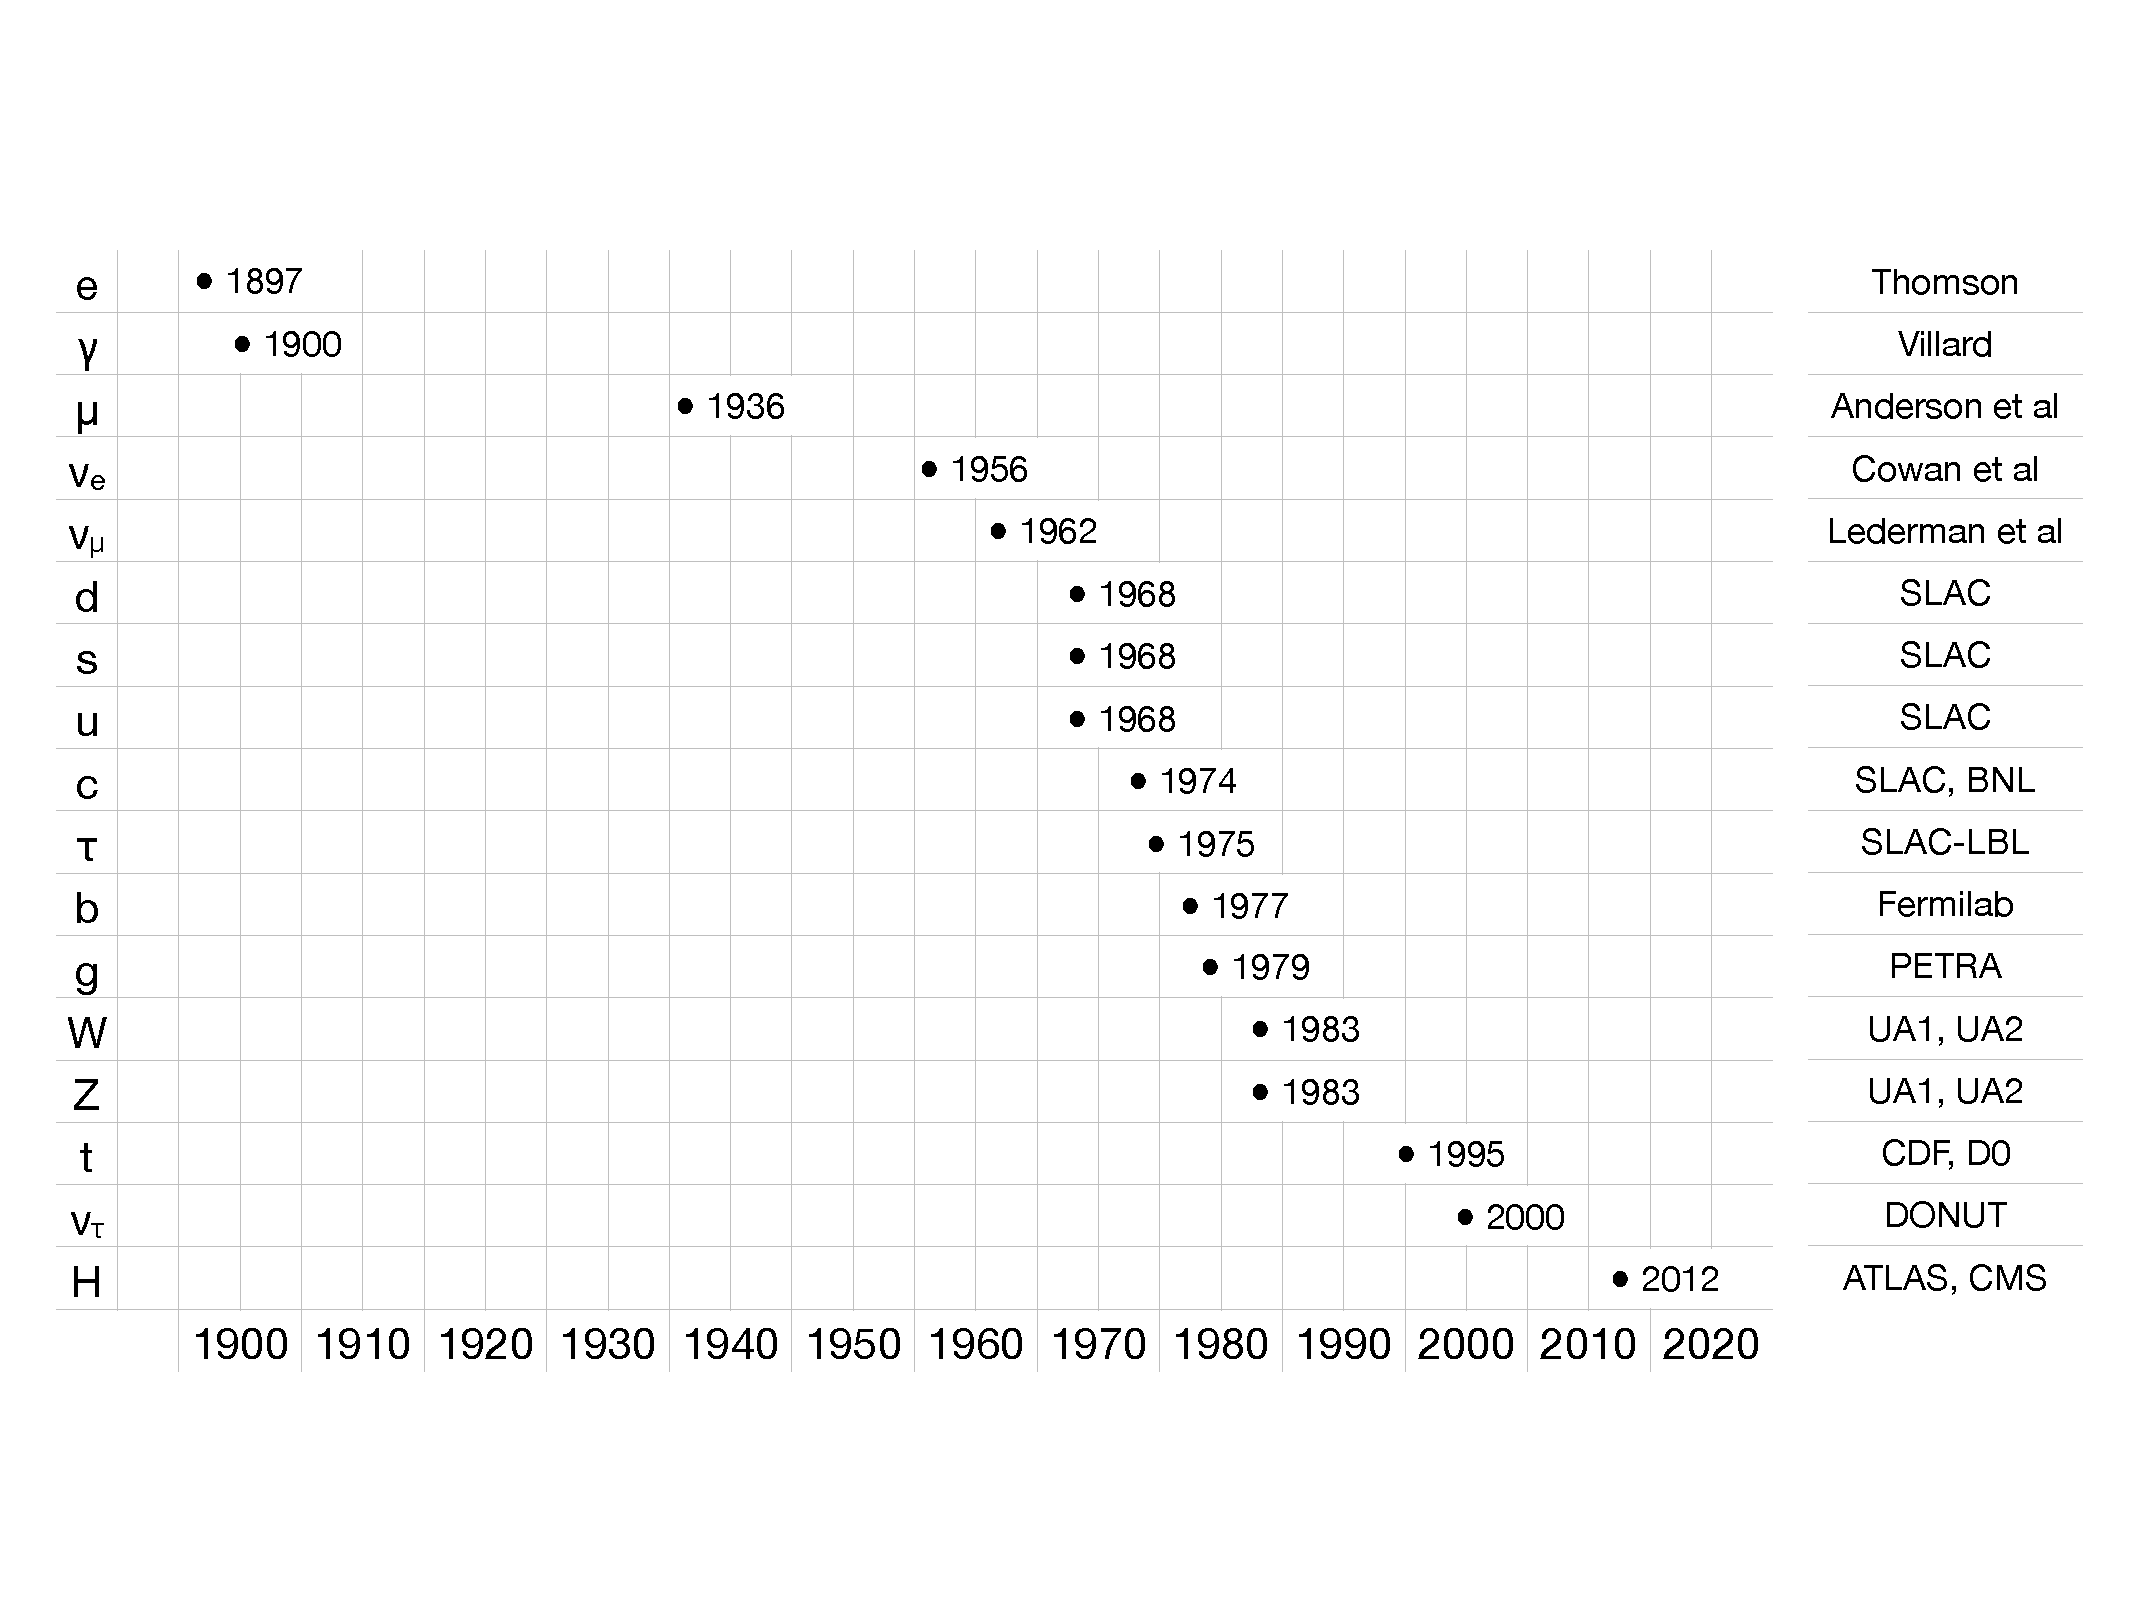
\includegraphics[width=0.90\textwidth]{figures/intro/discoveries.pdf}
      \end{center}
\caption{The discoveries of fundamental particles versus time~\cite{Tuna:thesis}.}
\label{fig:discoveries}
\end{figure}

In this theory, particles are treated as excitations of fields having half-integer spin or
integer spin, and the forces are treated as interactions among excitations of these fields.
The spin-$\frac{1}{2}$ particles, or fermions, can be divided into groups based on the ways
in which they interact. The leptons, or those particles which only experience the electroweak force,
are the electron $e$, muon $\mu$, tau $\tau$, electron neutrino $\nu_e$, muon neutrino $\nu_\mu$, and
tau neutrino $\nu_\tau$. The quarks, or those particles which experience both electoweak and strong
forces, are the up $u$, down $d$, strange $s$, charm $c$, bottom $b$, and top $top$. The integer-spin
particles, or bosons, are the spin-1 photon $\gamma$, $W$, $Z$, and gluon $g$ and the spin-0 Higgs $H$.
The particle content of the SM is summarized in Figure~\ref{fig:SMtable}.

\begin{figure}[ht]
 \begin{center}
    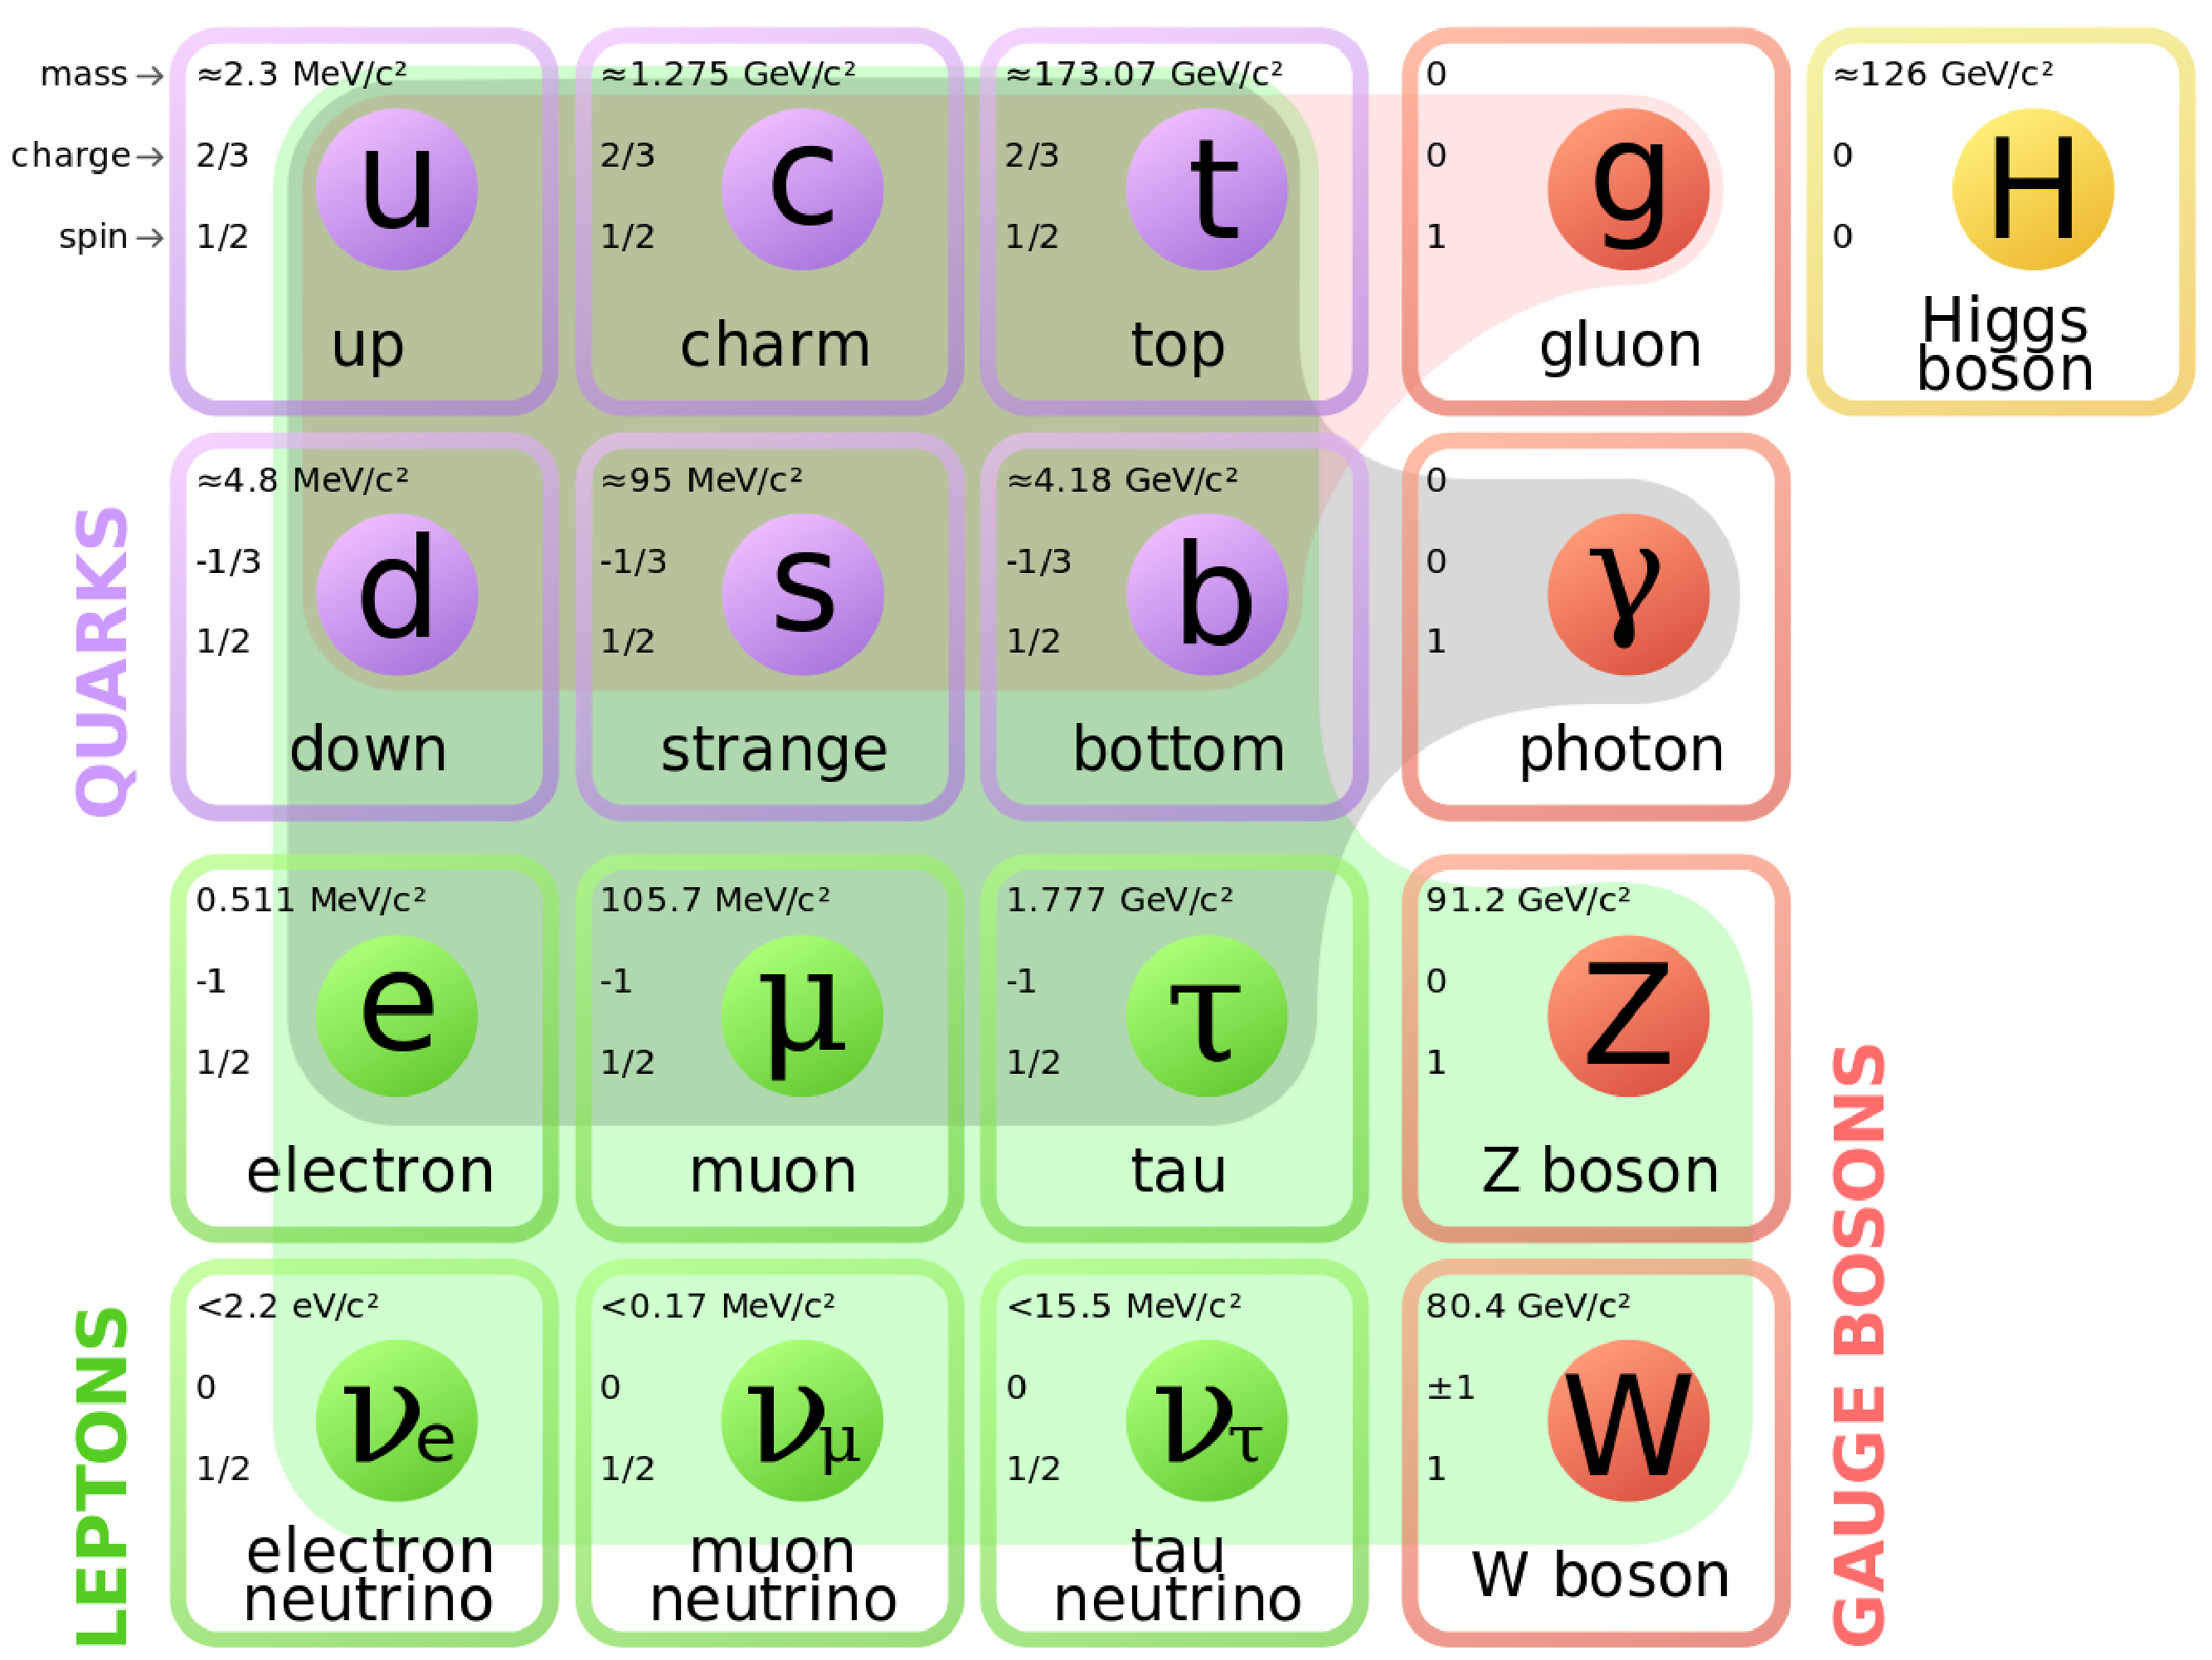
\includegraphics[width=0.90\textwidth]{figures/intro/Standard_Model_of_Elementary_Particles_modified_version.pdf}
      \end{center}
\caption{A diagram of the particle content of the SM~\cite{SMdiagram}.
The mass, electric charge, and spin is given for each, and the background color indicates how each
fermion interacts with the bosons.}
\label{fig:SMtable}
\end{figure}

The dynamics of the SM are described through its Lagrangian, which is invariant under
gauge transformations of the group $\text{SU(3)}_C \times \text{SU(2)}_L \times \text{U(1)_Y}$.
The strong force is associated with transformations under $\text{SU(3)}_C$, which give rise to
the conserved color charge $C$, denoted red, green, or blue, and eight gauge fields.
The group acts on 18 spinor fields corresponding to the quarks (six quark flavors in three colors)
and the eight gauge fields corresponding to the gluons.
The electroweak force is associated with transformations under $\text{SU(2)}_L \times \text{U(1)_Y}$,
the first part of which give rise to the conserved left-handed chirality $L$ and three gauge fields,
and the second part of which gives rise to the conserved weak hypercharge $Y$ one gauge field.
This group acts on left-handed doublets and right-handed singlets of the quarks, leptons, and
these four gauge fields. The quarks contribute nine doublets and 18 singlets, and the leptons contribute
three doublets and three singlets (as right-handed neutrinos do not exist).

The symmetry group of the SM does not allow for gauge-invariant mass terms. Instead,
the generation of particle masses is accomplished through the partial breaking of the
symmetry group by the addition of the Higgs field and potential, after which gauge-invariant
Yukawa interactions between fermions and the Higgs field naturally give fermion masses.
The Higgs field is a doublet of $\text{SU(2)}_L$. blah


\section{Higgs Discovery\label{sec:discovery}}
reference by sec:CMS

\section{Successes of the SM\label{sec:SMsuccess}}

\section{Shortcomings of the SM\label{sec:SMshortcomings}}
reference by sec:CMS


\section{diHiggs as a probe of SM and New Physics\label{sec:diHiggs}}




\chapter{Experimental Facility\label{ch:experiment}}

\section{CERN\label{sec:CERN}}
overview of facilities, experiments, history

\section{LHC\label{sec:LHC}}
proton beams, how do they work?

\section{CMS\label{sec:CMS}}
plenty of subsections here for tracker, ecal, hcal, solenoid, muons
talk about trigger and storage later


\chapter{Big Data\label{ch:data}}

The LHC delivers $pp$ collisions at a very high rate, much higher than CMS can read out or store
offline. From all these collisions, CMS selects a subset of events many order of magnitudes smaller
which are the most relevant for the physics processes of interest. This task is accomplished
through the trigger system, which is discussed in Section~\ref{sec:trigger} both in general and
in the context of this analysis. The events selected by the trigger system compose the datasets
used by all CMS analyses. The worldwide computing grid for storage and processing of both datasets
and simulation samples is disussed in Section~\ref{sec:storage}. Finally, the simulation samples
employed by this analysis are discussed in Section~\ref{sec:sim}.


\section{The Trigger System\label{sec:trigger}}

The gap in time between successive bunch crossings by the LHC is 25 ns, which is equivalent to
a frequency of 40 MHz. This large rate is reduced by selecting only the most interesting events
in a two-level trigger system. The first level, Level 1 (L1), is hardward-based and reduceds the
total event rate from 40 MHz to 100 kHz~\cite{Bayatyan:706847}, whereas the second level,
the High Level Trigger (HLT) is software-based and reduces the total event rate from 100 kHz to
100 Hz~\cite{Virdee:1043242}. From here, the events are processed further and stored
for the physics analyses.

The L1 trigger attempts to identify basic physics objects based on coarse energy deposits in
ECAL or HCAL or
based on collections of hits in muon chambers. By scanning the energy deposited in the calorimeters,
quantities derived from the sum of energy deposited, such as the missing transverse energy $\met$.
The Level 1 global trigger (GT) combines these object candidates and derived quantities in order
to select events to pass the the HLT with a processing time of $3 \mu$s.
Up to 128 separate trigger paths may be supported.

The HLT is able to access more information than the L1 trigger, and in doing so it can provide
a better description of the event. At the HLT level, tracker information is used in conjunction with
the full granularity of ECAL and HCAL. Information at this level is based on the presence of one or
more candidate objects satisfying requirements based on their transverse momentum or energy and relative
or absolute positions in the detector. With this added complexity and fewer events to process,
the average processing time is 40 ms.

\subsection{The Trigger for $\ggbb$}

In the search for the $\ggbb$ final state, this analysis can be viewed as an extension of the
SM $\Hgg$ search~\cite{HggCMSpaper}. The excellent diphoton mass
resolution is the principle driver in the sensitivity since it allows for low background contamination
in the signal region, as will be shown in Chapter~\ref{ch:results}.
Therefore, the trigger strategy centers on the ability to find two high-quality photon candidates.

During 2012 data taking, the LHC luminosity increased over time, and the triggers at both L1 and HLT
had their thresholds increased in order to keep the event rates within the limits of the two levels.
The requirement at L1 is for two $e/\gamma$ candidates with $E_{\rm T}$ requirements of 13 (7) GeV
for the lead (sublead) candidate or for one $e/\gamma$ candidate with an $E_{\rm T}$ requirement of
22 GeV.

At HLT events are selected through diphoton triggers with asymmetric $E_{\rm T}$ thresholds
and complementary photon selections. One trigger selection requires a loose calorimetric
identification based on the shape of the electromagnetic shower and loose isolation requirements
on the photon candidates, while the other requires that the photon electromagnetic shower
is primarily concentrated in a three-by-three crystals super-cluster.
The trigger thresholds on the photon $E_{\rm T}$ are 26 (18) GeV and 36 (22) GeV on the leading
(subleading) photon, depending on the acquisition period of LHC data taking in 2012.
The path with the 26 (18) GeV thresholds is initiated by the L1 path with 13 (7) GeV thresholds, while
the path with 36 (22) GeV thresholds is initiated by the L1 path with a single 22 GeV threshold.

In addition to keeping the trigger rate within its limits, it is also neccessary to set thresholds
low enough such that the selection of signal events remains as high as possible. This trigger efficiency
is studied on Monte Carlo (MC) signal samples as well as on $Z\rightarrow e^+ e^-$ data.
For the study on MC, the efficiency is above 99.5\% for all conditions of 2012 data taking.

Figures~\ref{fig:ZeeTriggerPt} and \ref{fig:ZeeTriggerNvtx}
show how the trigger efficiency varies on data with respect to the
candidate photon $p_{\rm T}$ and the number of primary vertices in the event
using the tag and probe technique. To account for differences
between the shower shape between photons and electrons, the data sample was reweighted to match the
shower shapes. Within uncertainties, the trigger efficiency is higher than 99\% for the 2012 data.

\begin{figure}[ht]
 \begin{center}
    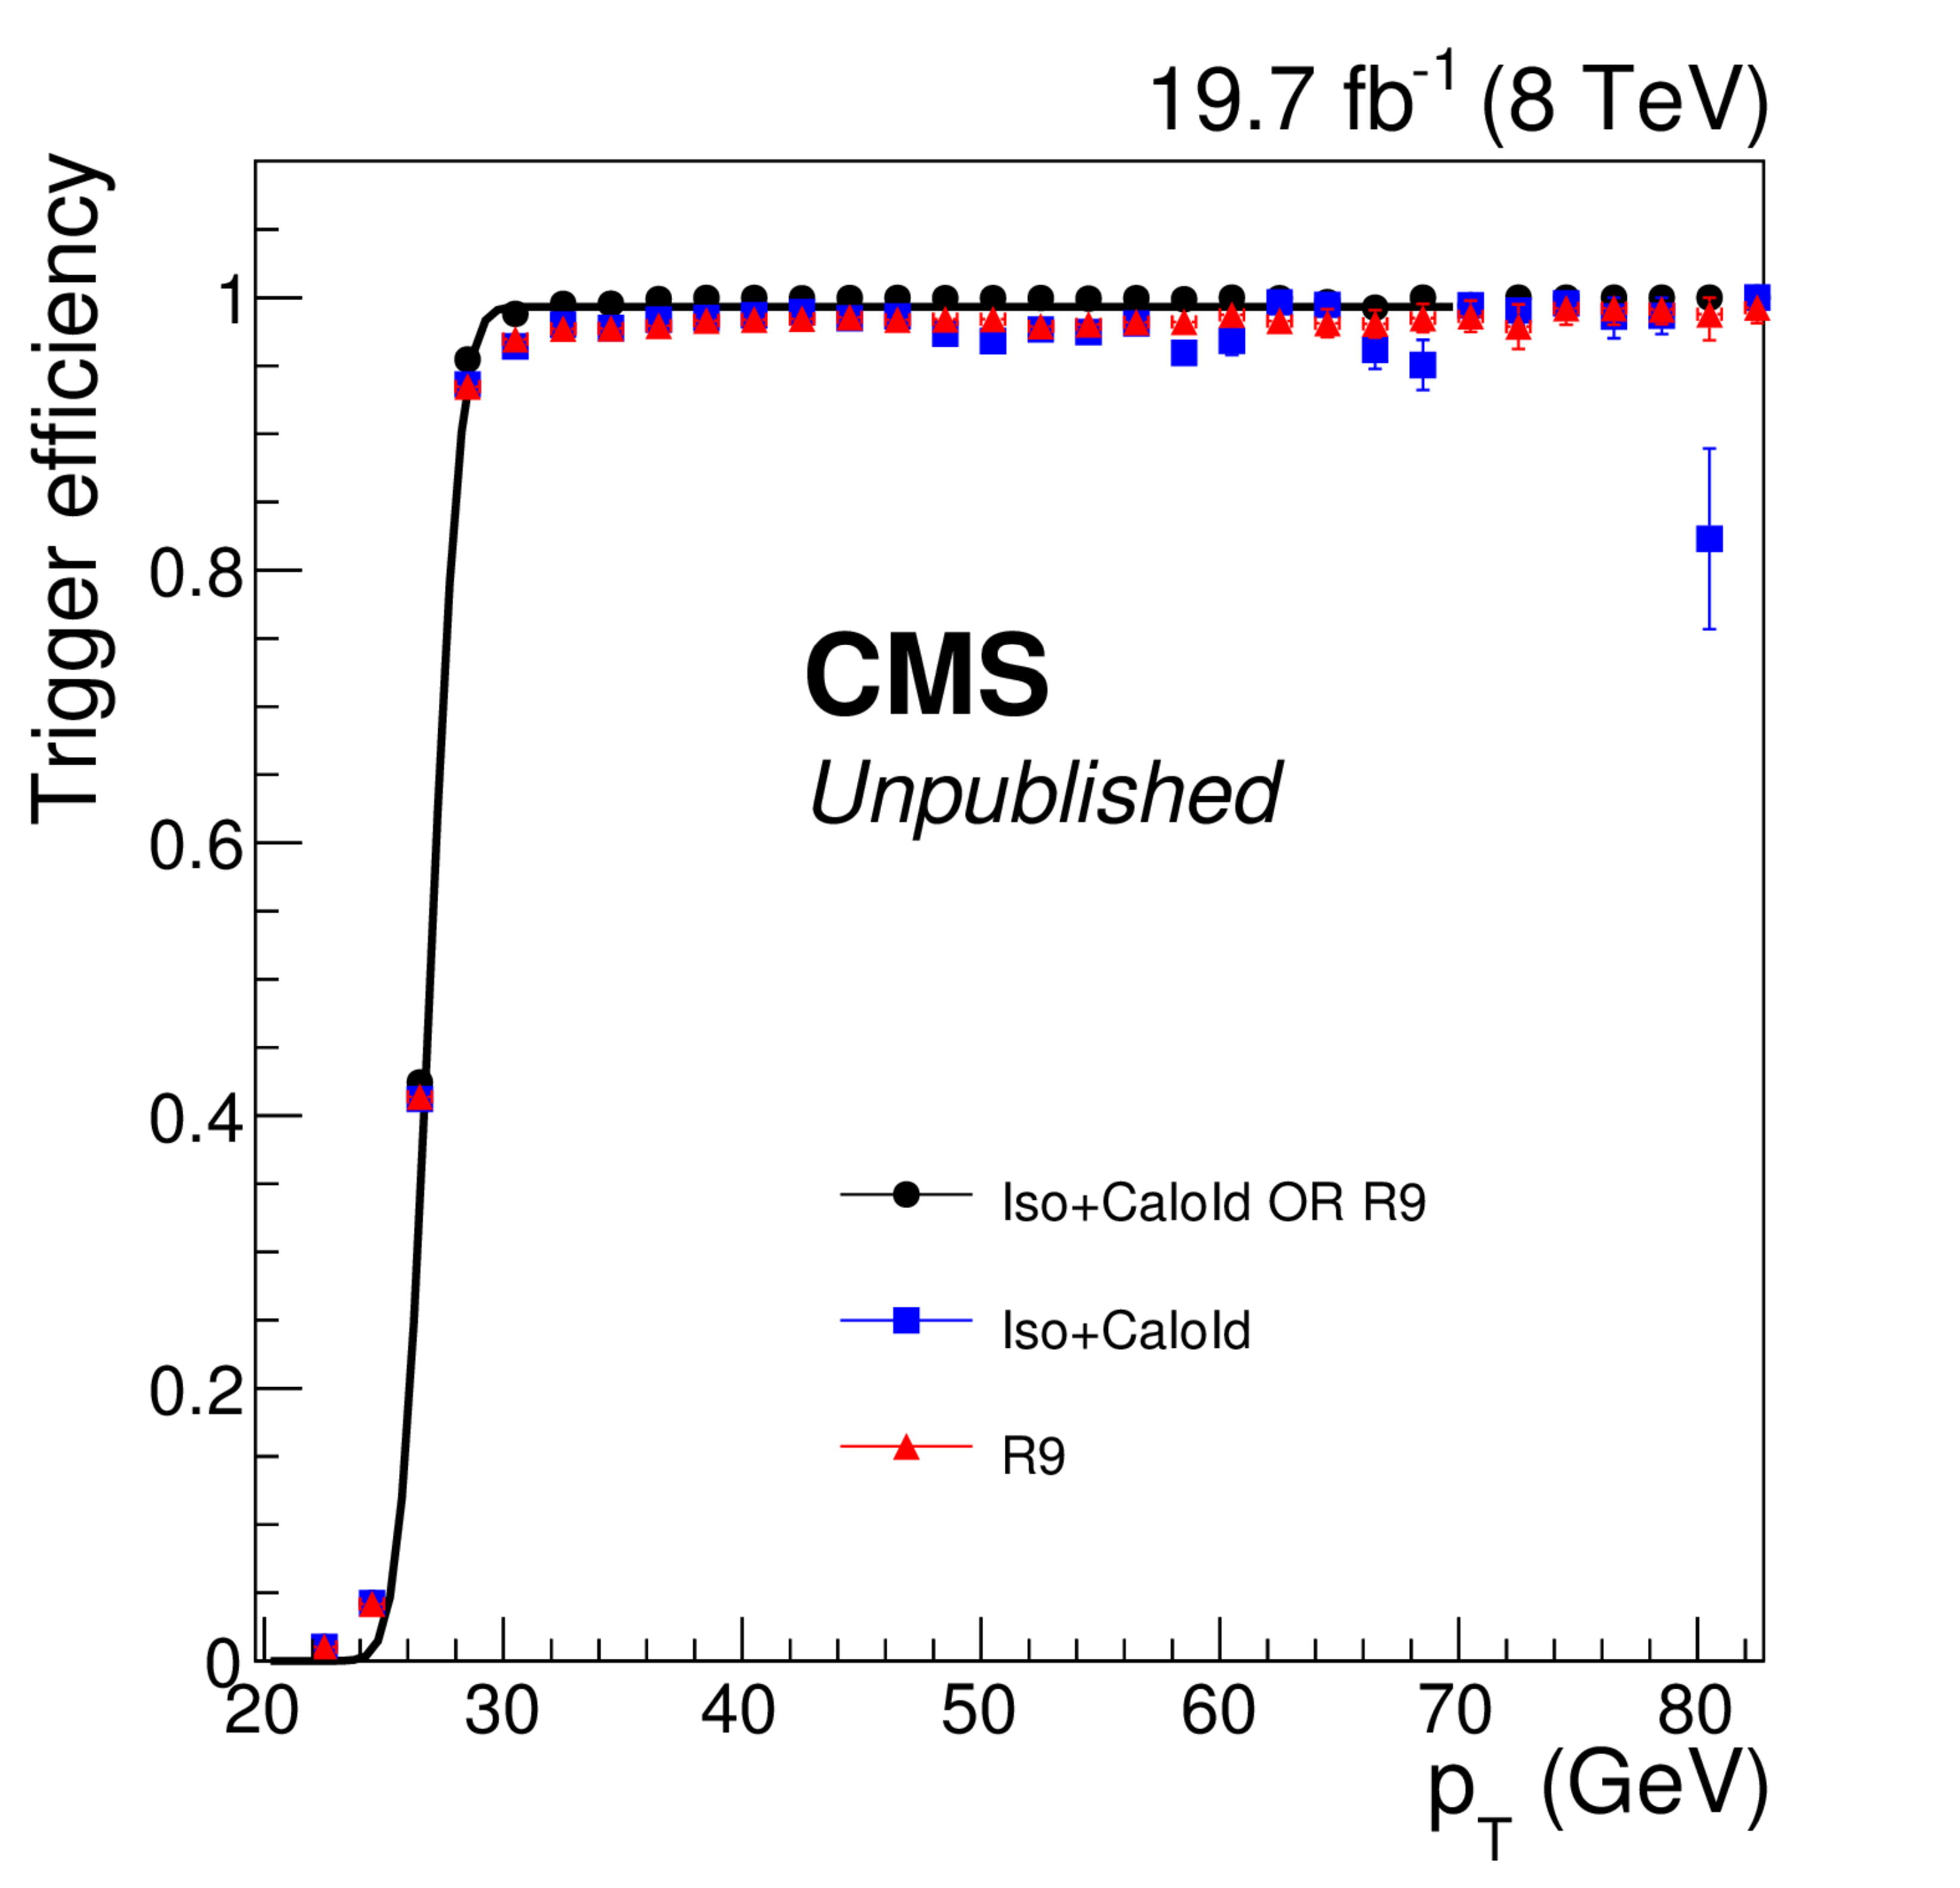
\includegraphics[width=0.60\textwidth]{figures/data/turnon_pt.pdf}
      \end{center}
\caption{Efficiency of the trigger selection as a function of the photon candidate transverse
momentum measured in $Z\rightarrow e^+ e^-$ events~\cite{HggCMSpaper}.}
\label{fig:ZeeTriggerPt}
\end{figure}

\begin{figure}[ht]
 \begin{center}
    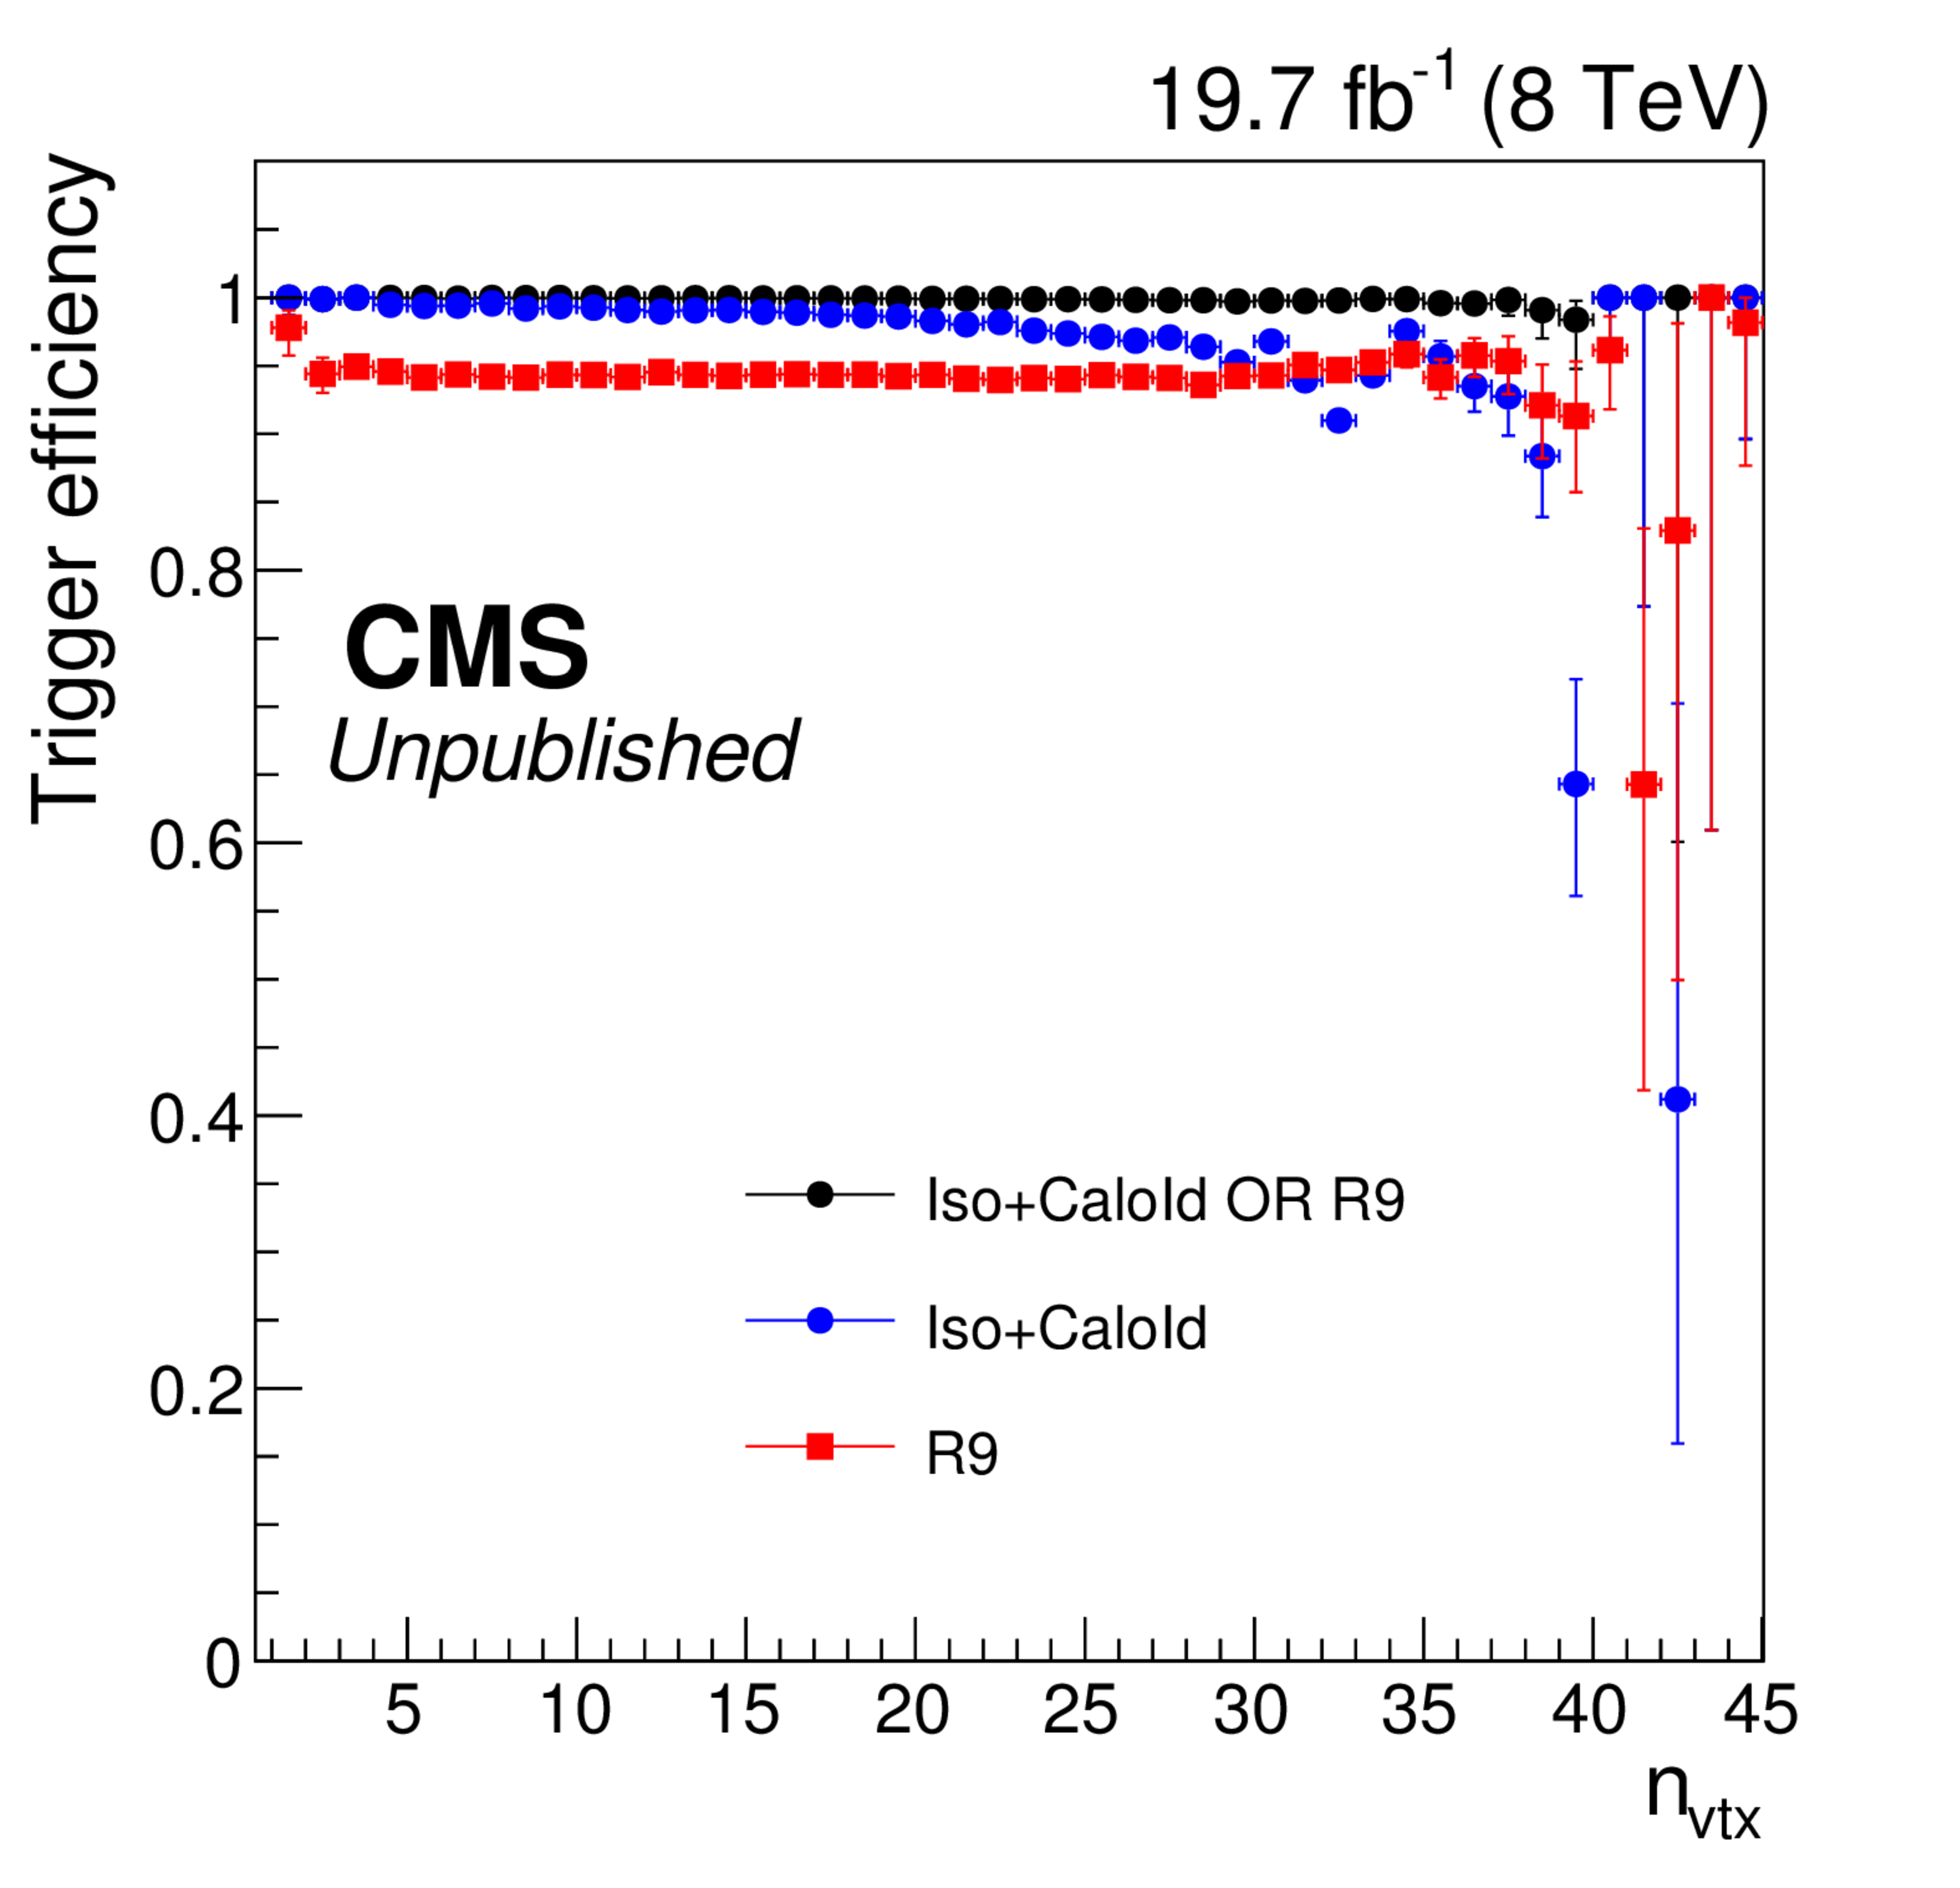
\includegraphics[width=0.60\textwidth]{figures/data/turnon_nvtx.pdf}
      \end{center}
\caption{Efficiency of the trigger selection as a function of the number of primary vertex in the event
measured in $Z\rightarrow e^+ e^-$ events~\cite{HggCMSpaper}.}
\label{fig:ZeeTriggerNvtx}
\end{figure}


\section{Data Storage Worldwide\label{sec:storage}}

All the data from the LHC and its experiments, including CMS, is processed, stored, and analyzed
in a distributed global collaboration of computing centers~\cite{Eck:840543}. The Worldwide
LHC Computing Grid (WLCG) is the world's largest computing grid, composing of over 170 centers
arranged in a tier structure. Part of this tier structure is shown in Figure~\ref{fig:cerncomputing}

\begin{figure}[ht]
 \begin{center}
    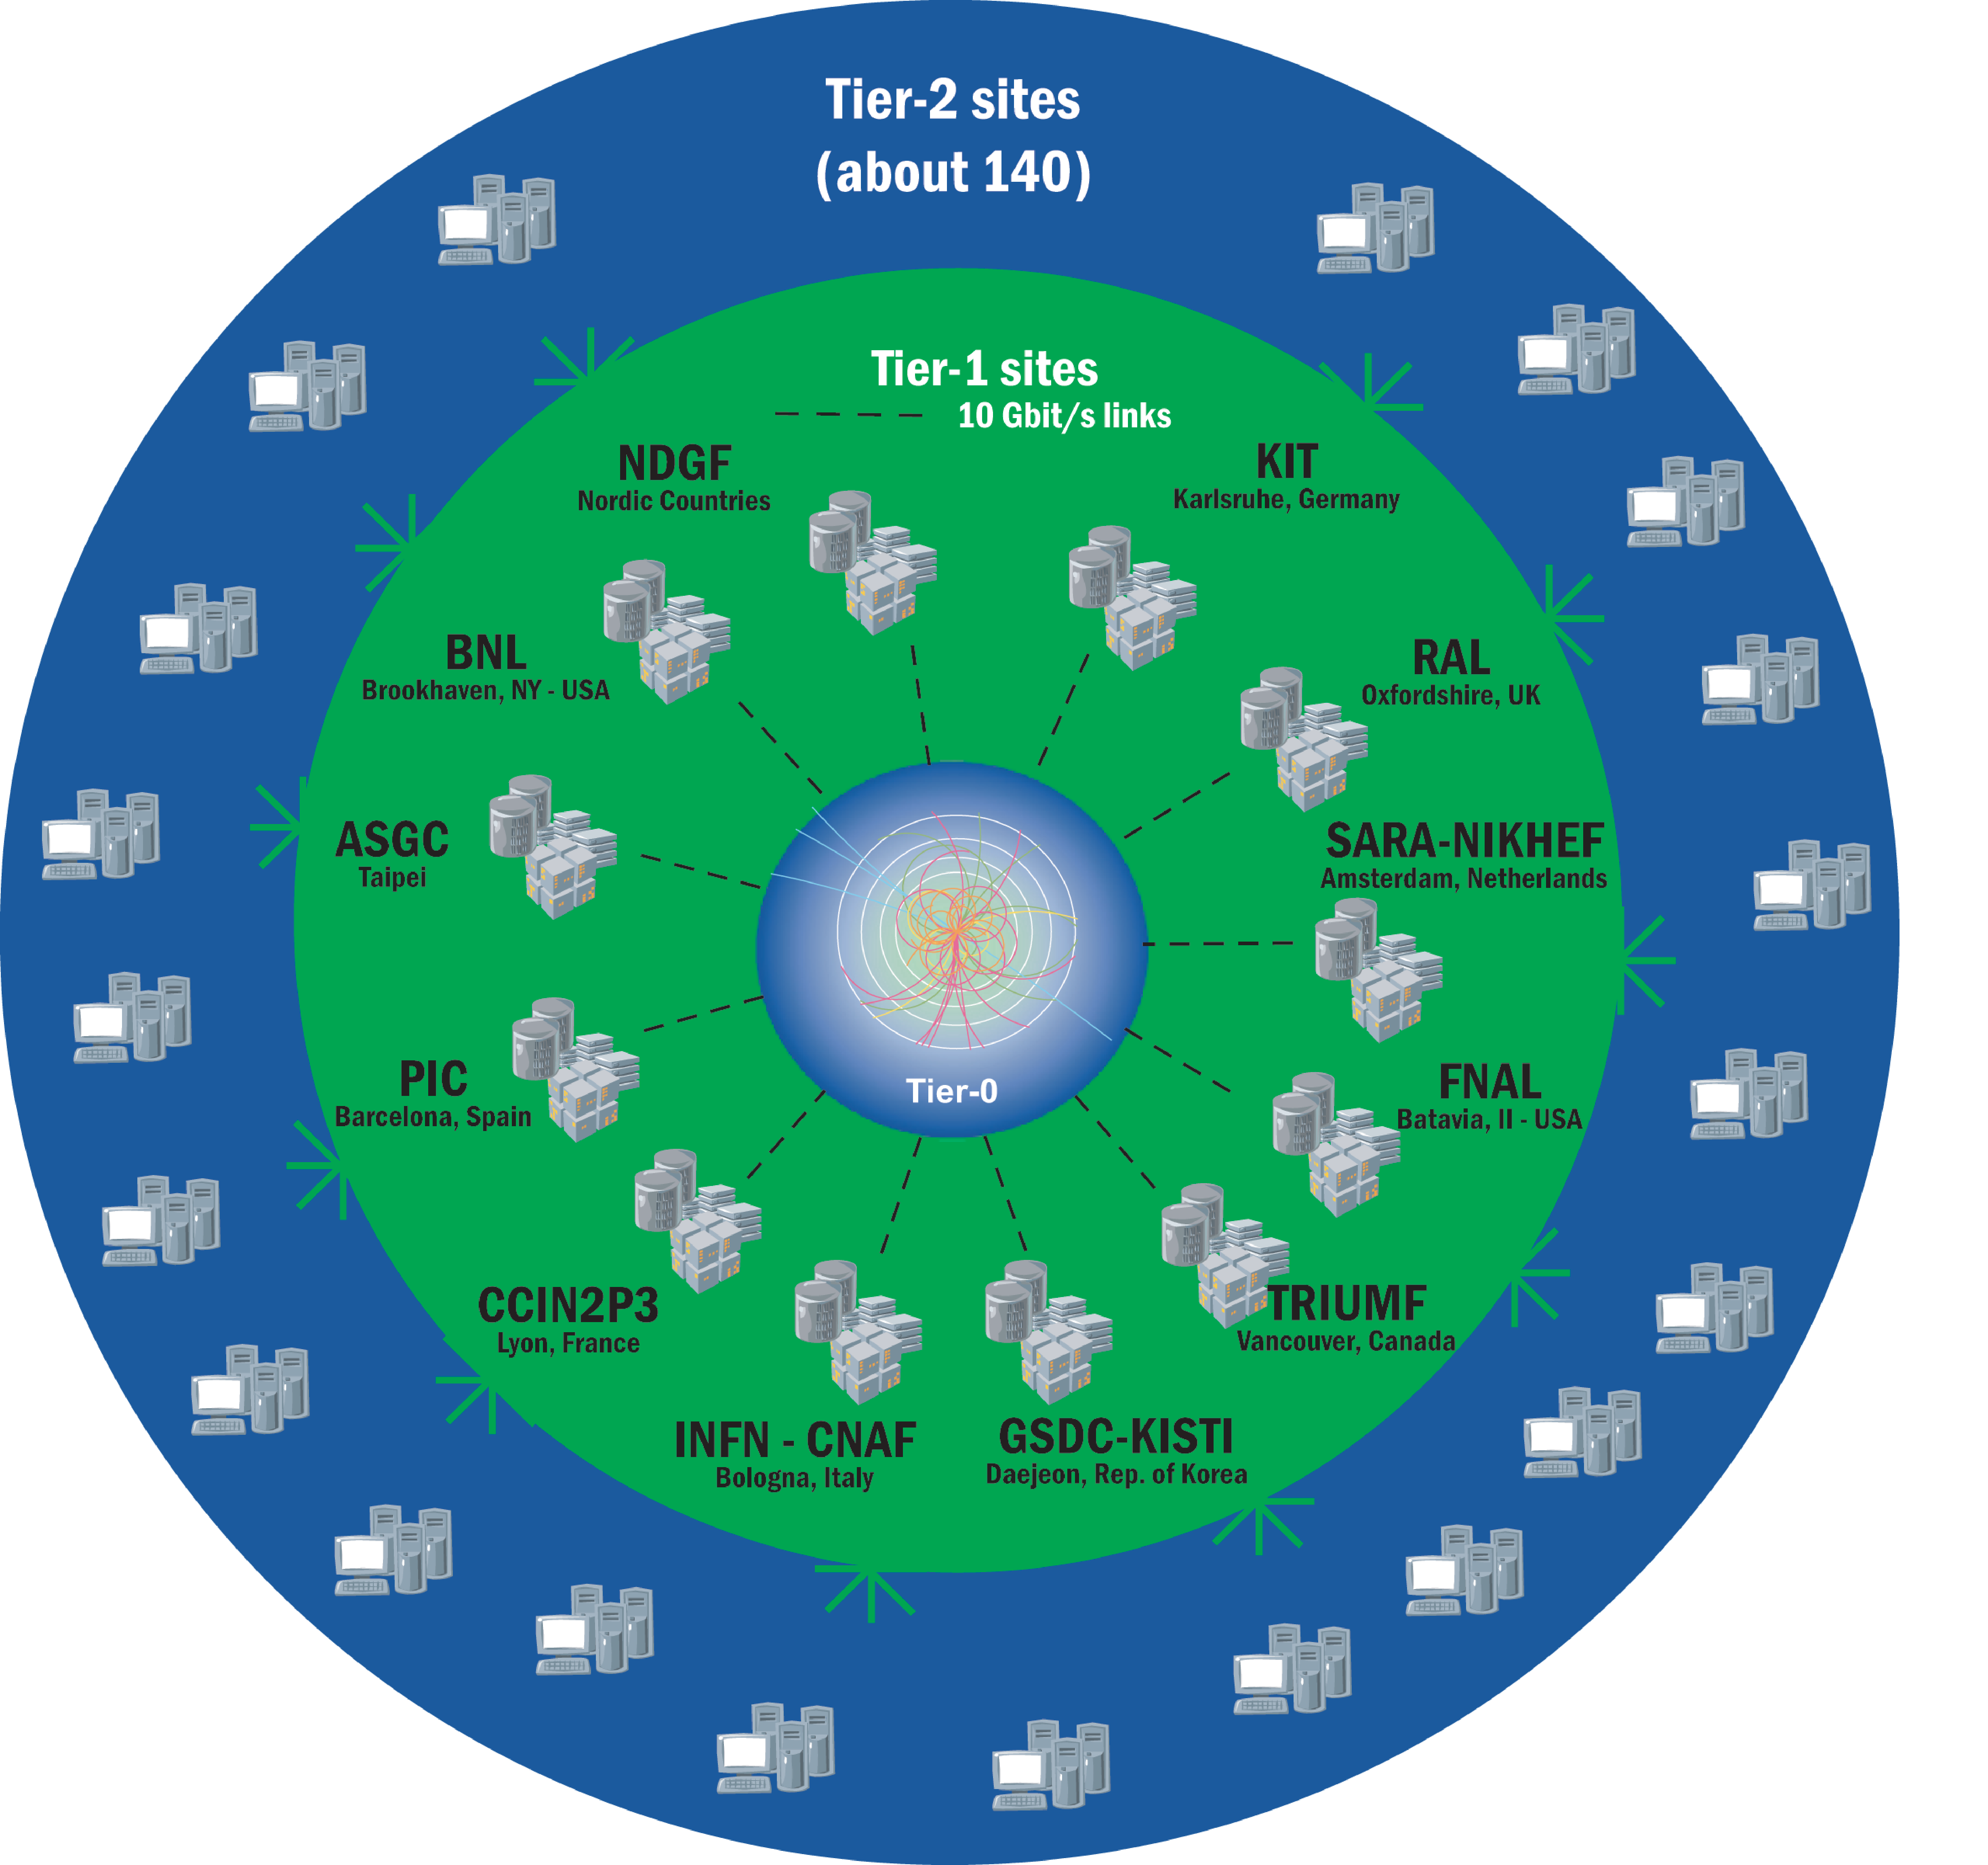
\includegraphics[width=0.70\textwidth]{figures/data/CCApr13-Tiers0-1-2_PNG-file.pdf}
      \end{center}
\caption{A schematic of the WLCG detailing the locations of the Tier-1 sites~\cite{cern:computing}.}
\label{fig:cerncomputing}
\end{figure}

Tier 0 is the CERN Data Center, through which all LHC data passes for initial processing and
reconstruction. The raw and processed data from Tier 0 is pushed to one of the 13 Tier 1 sites, where
later reprocessing and storage can be done. From here, the Tier 1 sites push the reconstructed
datasets to Tier 2 sites for storage and processing by analysts. This system handles the approximately
30 Petabytes of data generated per year by the LHC experiments in addition to the large amount of
MC samples generated and stored.

\section{Simulation Samples\label{sec:sim}}

%include more theory details on radion, graviton, mssm used in the sample generation

MC simulation samples are employed to study signal and background processes in more detail
than would be offered by data alone. In a search for some new signal process, there is a trade-off
between optimizing an analysis for one particular new physics scenerio and the ability to
generalize a result to other signal processes. This analysis generally searches for a double Higgs final
state by optimizing strategies separately between the resonant and nonresonant production mechanisms.
The signal MC samples are discussed in Subsection~\ref{subsec:sig_samples}.
In addition, good agreement between data
and background MC serves as a validation that the major backgrounds are understood and that
the data is behaving as expected. The background MC samples are discussed in
Subsection~\ref{subsec:bkg_samples}.

\subsection{Signal Simulation\label{subsec:sig_samples}}

\subsection{Background Simulation\label{subsec:bkg_samples}}



\chapter{Physics Objects\label{ch:objects}}

After data is selected by the trigger, the offline analyses begin with particle identification.
There are no longer any timing limitations, so such identification can make use of all the detector
information in the event. To this end, CMS uses the Particle Flow (PF) algorithm
in most analyses, which is described in Section~\ref{sec:PF}.
As this search for double Higgs production centers around the identification of
events with both $\Hgg$ and $\Hbb$ decays, the
identification and reconstruction of photons and jets are the first steps taken after the
trigger selects potentially-interesting events,
and this chapter discusses the treatments needed at this stage for both data and MC samples.
Recalling that the sensitivity in the separation between signal and background comes from the
excellent diphoton mass resolution, the identification of two high quality photons is the starting point
and discussed in Section~\ref{sec:photons}. The following step is the identification of two jets
coming from the hadronization of b-quarks and is discussed in Section~\ref{sec:jets}.


\section{Particle Flow\label{sec:PF}}

The PF algorithm reconstructs all stable particles in an event from the digitized electronic signals
of all channels in all subsystems~\cite{PFPAS2009,CMS-PAS-PFT-10-001}. These particles include
electrons, photons, charged hadrons, neutron hadrons, and muons, as shown in Figure~\ref{fig:PF}.
From these particles, derived objects are constructed, including jets and missing transverse energy.
The algorithm itself links detector objects created from individual subsystems and groups them into
blocks that are identified with a particle. The detector objects are discussed in
Section~\ref{subsec:detobj}, the linking of these objects is discussed in Section~\ref{subsec:linking},
and the identification of groups of these links with particles is discussed in
Section~\ref{subsec:groupid}.

\begin{figure}[ht]
 \begin{center}
    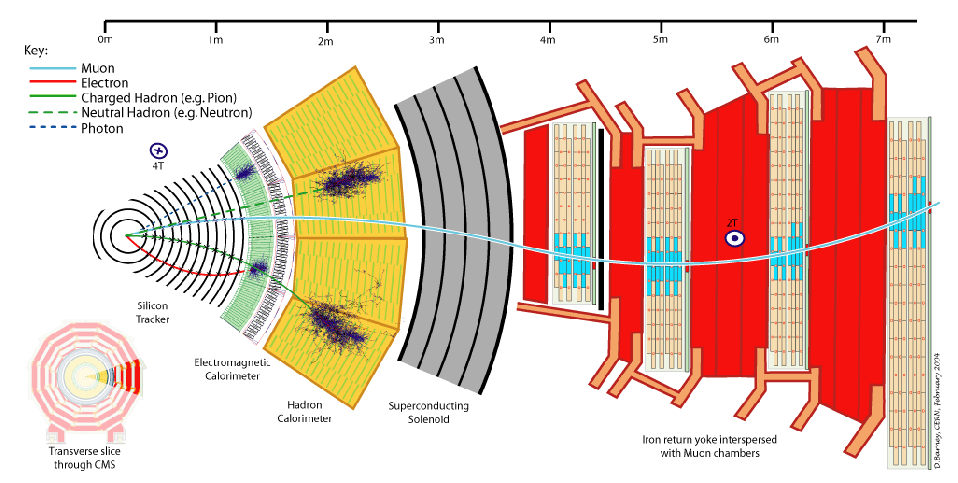
\includegraphics[width=0.95\textwidth]{figures/objects/pf.pdf}
      \end{center}
\caption{A schematic of a slice of the CMS detector in the plane transverse to the beam line.
The trajectories of an electron, photon, charged hadron, neutral hadron, and muon are superimposed
with the interactions that each of these particles has with the various subsystems.}
\label{fig:PF}
\end{figure}

\subsection{Detector Objects\label{subsec:detobj}}

The first step of the PF algorithm is to assemble detector objects created separately from
individual subsystems. In the tracker, hits in pixels or strips are associated into a track candidate
through the iterative Combinatorial Track Finder algorithm~\cite{PFPAS2009}. In the muon chambers,
standalone muon tracks (to distinguish from tracks formed by tracker hits)
are assembled from hits in the three muon detectors, accounting
for the nonuniform magnetic field and large detector budget and constraining a track candidate to
intersect the beamline. In the ECAL and HCAL, clustering of energy deposits is performed around a
cluster seed, which is identified as a detector unit with an amount of energy exceeding a
detector-dependent threshold and corresponding to a local maximum relative to neighboring units.
Units are then added to adjacent seeds if their energy exceeds a noise threshold,
and the PF clusters are
formed by redistributing the the energy back to the cluster seeds, recalculating the position as a
weighted average over the energy of each contributing cluster.

\subsection{Linking\label{subsec:linking}}

The next step of the PF algorithm is to link the detector objects to assemble PF candidates.
Possible links are between a track and standalone muon track, between a track and a cluster, and
between two clusters, each having their own associated linking parameters. A link is formed between
a track and standalone muon track when the two can be merged into a global track with a fit
having $\chi^2$ below a certain threshold. A link is formed between a track and a cluster when
the extrapolation of the track is within a certain distance of the cluster position.
A link is formed between two clusters
(either both in ECAL, both in HCAL, or one in each) when the two clusters are within a certain distance
to each other.

\subsection{Grouping and Identification\label{subsec:groupid}}

An ensemble of links creates a block, and identification proceeds iteratively through PF candidates.
First, muons are identified from those blocks that contain a global track having a momentum
sufficiently close to the momentum of the contained track. Then electrons are identified from blocks
containing a track and an ECAL cluster where the track and energy cluster satisfy requirements
consistent with the signature of an electron. Next photons and hadrons are identified from blocks
containing a track and a cluster from either ECAL or HCAL. If the calibrated energy in the clusters is
greater than the sum of the momentum of the associated tracks, PF photons or PF neutrons are created
from the difference. If the difference is less than the energy in the ECAL clusters, a PF photon is
created from the block; if the difference is greater than the energy in the ECAL clusters,
a PF photon and a PF neutral hadron are made from the excesses ECAL and HCAL energy, respectively.
Finally, if the calibrated energy in the clusters is less than the sum of the momentum of the associated
tracks, a search for fake tracks and additional muons in the block is performed, and what remains
in the block is a PF charged hadron.

From the list of PF candidates in an event, jets and taus are constructed by clustering nearby
hadrons. In this way, the clustering of PF hadrons represents the original quark or tau from the
underlying interaction. Missing transverse energy, which is a signature of one or more neutrinos
in the event and/or the mismeasurement of the energy of PF candidate, is obtained by
\begin{equation}
\met = - \sum_i \vec{p}_{{\rm T},i} \, ,
\end{equation}
where the sum is over all PF candidates in the event.

The treatment for photons is discussed in more detail in Section~\ref{sec:photons}. The construction
of jets from PF candidates is discussed in more detail in Section~\ref{sec:jets}. 


%Matching the muons to the tracks measured in the silicon tracker results in a transverse momentum
%resolution between 1 and 5\,\% for \pt values up to 1~TeV. The ECAL has an energy resolution better
%than 0.5\% for unconverted photons with transverse energies above 100~GeV.
%The HCAL, when combined with the ECAL, measures jets with a resolution
%$\Delta E/E \approx 100\,\% / \sqrt{E\,[\gev]} \oplus 5\,\%$.

\section{Photons\label{sec:photons}}

PF photon candidates are reconstructed from clustering individual units in the ECAL
and checking consistency with tracks.
The calorimeter signals are calibrated for several detector effects~\cite{CMS-PAS-EGM-10-005,ECALpaper},
providing the best energy resolution possible.
The energy scale is corrected in both data and simulation, while the photon energy is smeared in
simulation in order to reproduce the same energy resolution that is observed in data.

With the PF photon candidates in hand, additional requirements are imposed in order to further
separate prompt photons from fake photons originating from misidentified electrons or from jets.
These additional requirements include an electron veto, an upper threshold on the energy deposited
in HCAL in the region about the candidate, isolation, and the shower shape. The electron veto 
removes a photon if there is an electron candidate matching the photon ECAL cluster with no missing
hits in the tracker and with no matching reconstructed conversion.
Isolation requirements place
thresholds on the amount of ECAL energy deposited in a region about the cluster; these are both
detector based and PF based. Requirements on the electromagnetic shower shape include the
width of the shower in terms of ECAL detector units and
ratio of the amount of energy in a 3$\times$3 unit box around the cluster seed to that
around a 5$\times$5 unit box.

After the quality cuts, the two photons candidates are requested to satisfy the sliding asymmetric cuts
\begin{subequations}
\begin{equation}
p_{{\rm T},\gamma_1} > \frac{\Mgg}{3}
\end{equation}
\begin{equation}
p_{{\rm T},\gamma_2} > \frac{\Mgg}{4} \, ,
\end{equation}
\end{subequations}
where $p_{{\rm T},\gamma_1}$ and $p_{{\rm T},\gamma_2}$ are the transverse momenta of the
leading and subleading photons, respectively.
The fact that these requirements on the transverse momentum are scaled by the diphoton invariant mass
prevents turn-on effects which could distort the shape of the $\Mgg$ spectrum for low values of $\Mgg$.
Both photons have the requirement that their position be within the ECAL acceptance of
$\left|\eta\right| < 2.5$ with an exclusion on the ECAL gap between the barrel and endcaps.
In the case that there are more than two photons passing the identification and kinematic requirements,
the two with the largest $p_{\rm T}$ are chosen. After this choice, the diphoton mass is required to
be between 100 and 180 GeV.

Figure~\ref{fig:mgg_onlyhiggs} shows the resulting simulated distributions for the diphoton mass 
of the resonant signal and resonant backgrounds.
In the case of the resonant background, the sum
of all SM $\Hgg$ production mechanisms is shown as a single contribution.
Figure~\ref{fig:mgg_controlplot} shows the same
distribution for data and the sum of backgrounds. (Note that these figures include requirements
on jets, discussed in Section~\ref{sec:jets}.)
The resolution of the diphoton mass spectrum for the signal is a few GeV.

The two primary drivers in the diphoton mass resolution are the energy resolution
of the individual photons
and the direction of the photons from their origin, which is synonymous with the identification
of the vertex from which they were produced. Due to the presence of the $\Hbb$ decay in the search,
the tracks from the jets allow for the efficient identification of the correct vertex since photons
do not have tracks unless they undergo pair-conversion in the tracker.
The criterion for the vertex choice is that which has the largest $\sum_i p_{{\rm T},i}$, where
the sum is over all of the tracks associated to a particular vertex. With this criterion,
the relative contribution to the diphoton mass resolution due to the vertex choice is
negligible with respect to the energy resolution for individual photons.

\begin{figure}[ht]
 \begin{center}
   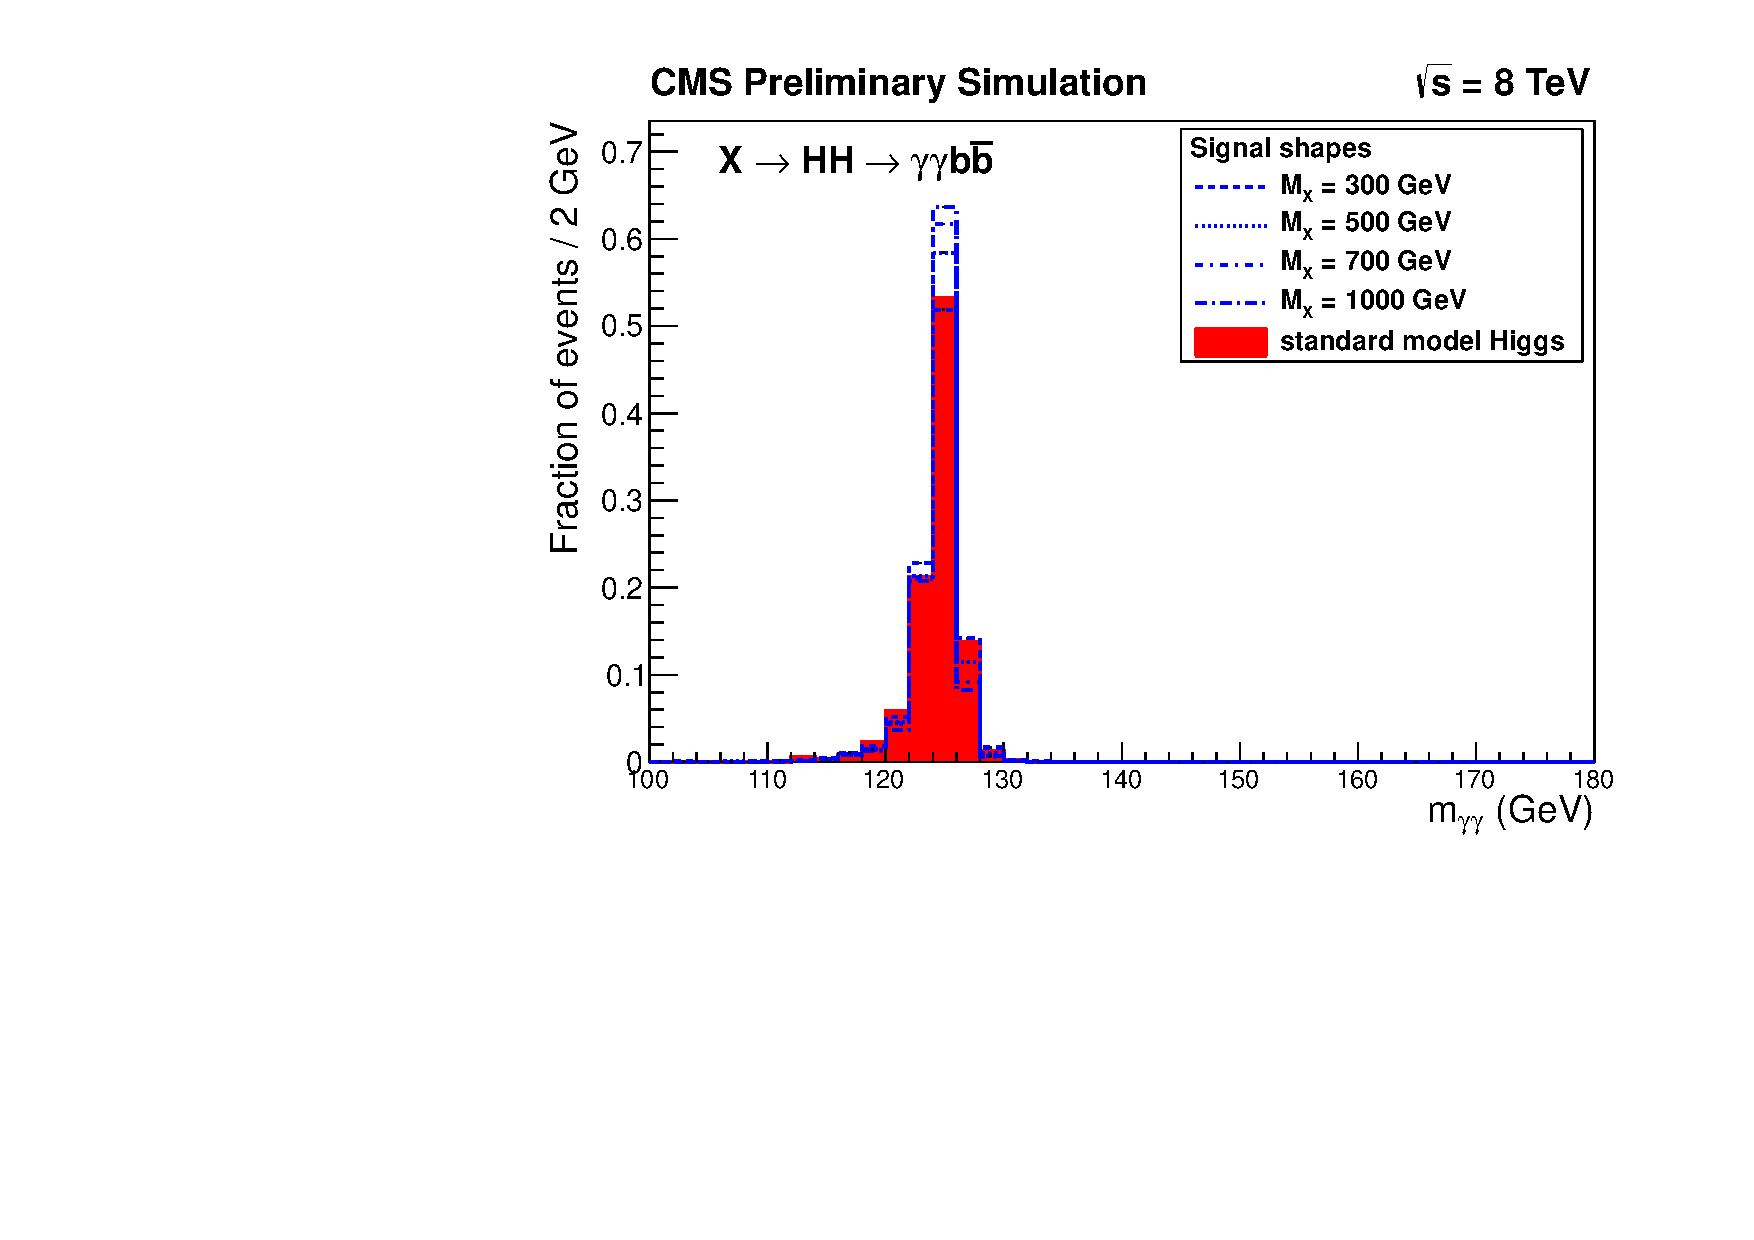
\includegraphics[width=0.70\textwidth]{figures/objects/DiPhotonMass_OnlyHiggs.pdf}
 \end{center}
\caption{Simulated diphoton mass spectrum for the resonant signal and the sum of all production
mechanisms of the
SM Higgs boson after basic selections on photons and jets and requesting at least
one loose b-tagged jet.
The spectra are normalized to one.}
\label{fig:mgg_onlyhiggs}
\end{figure}

\begin{figure}[ht]
 \begin{center}
   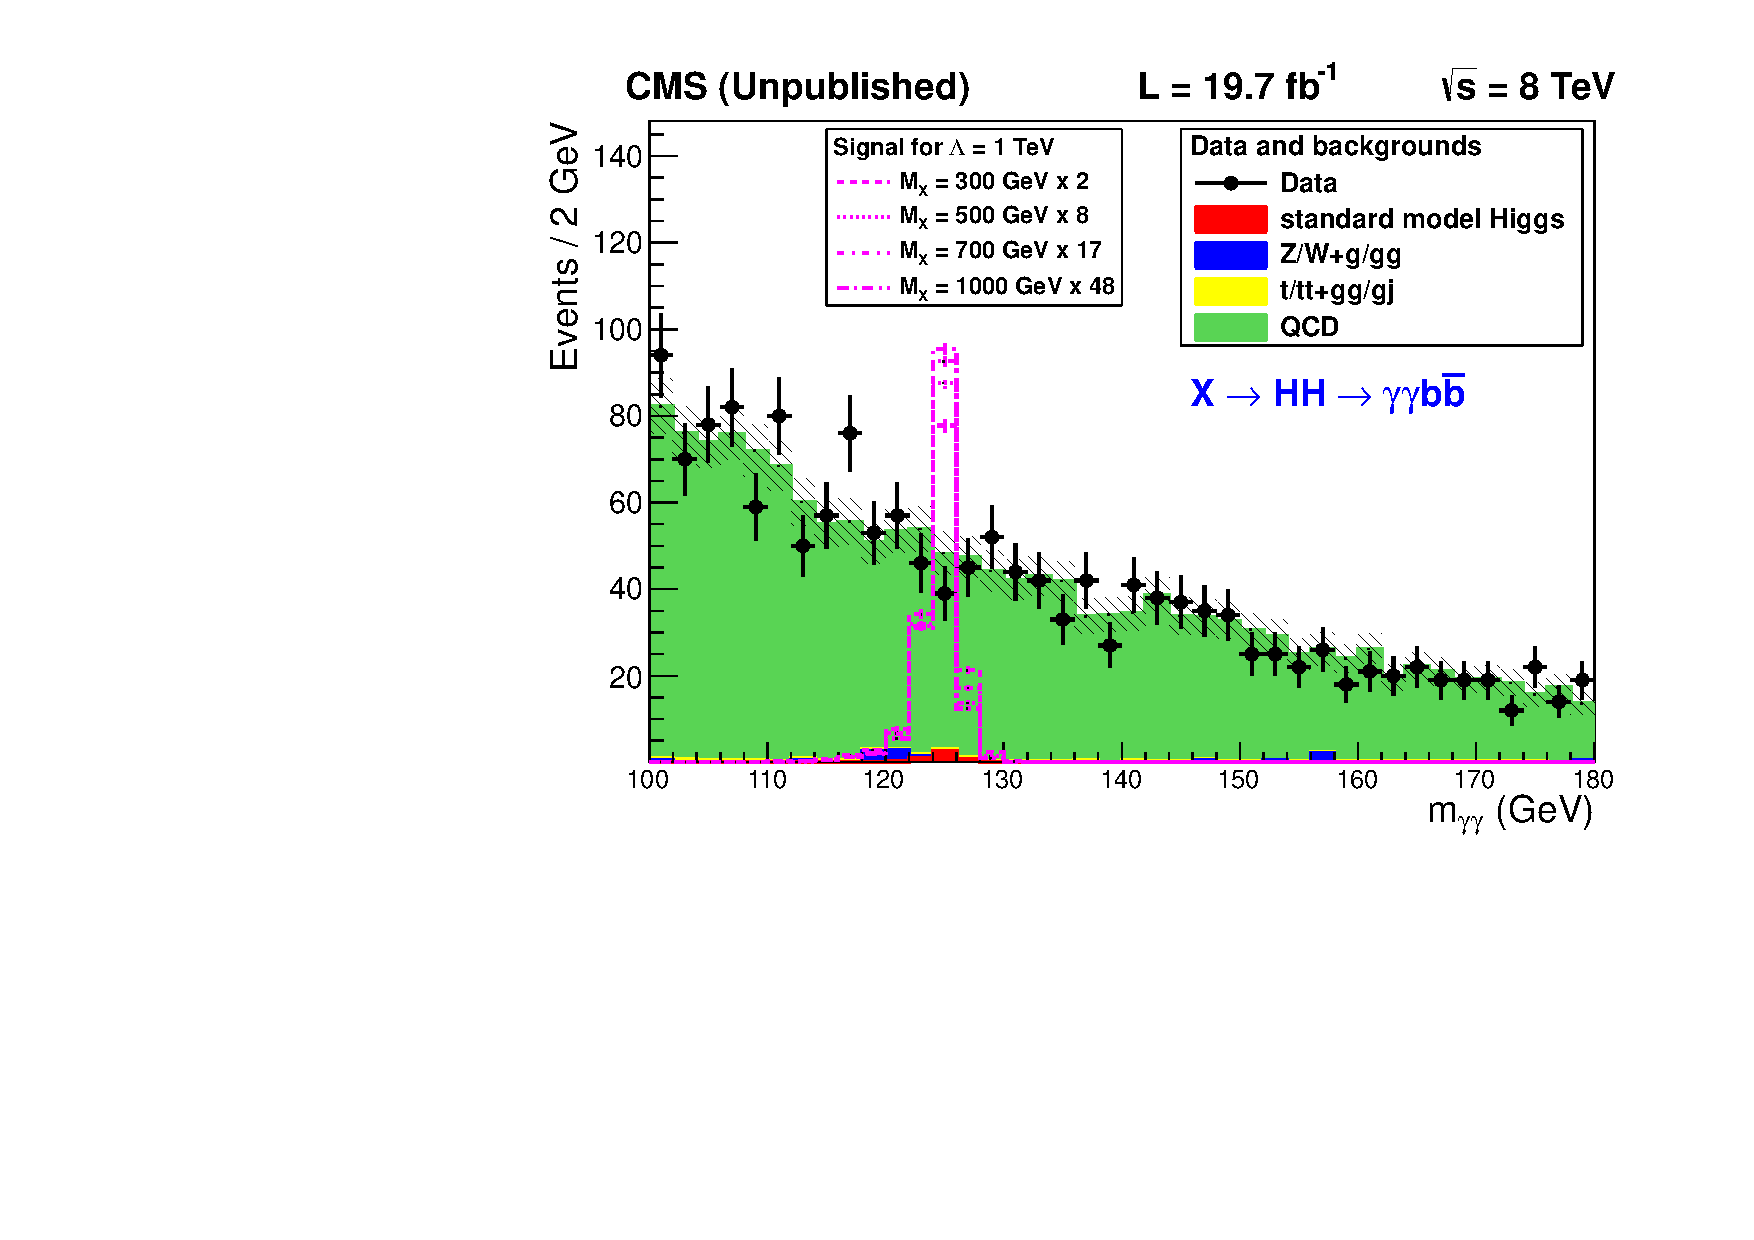
\includegraphics[width=0.70\textwidth]{figures/objects/DiPhotonMass_ShapeNormalized_sys.pdf}
   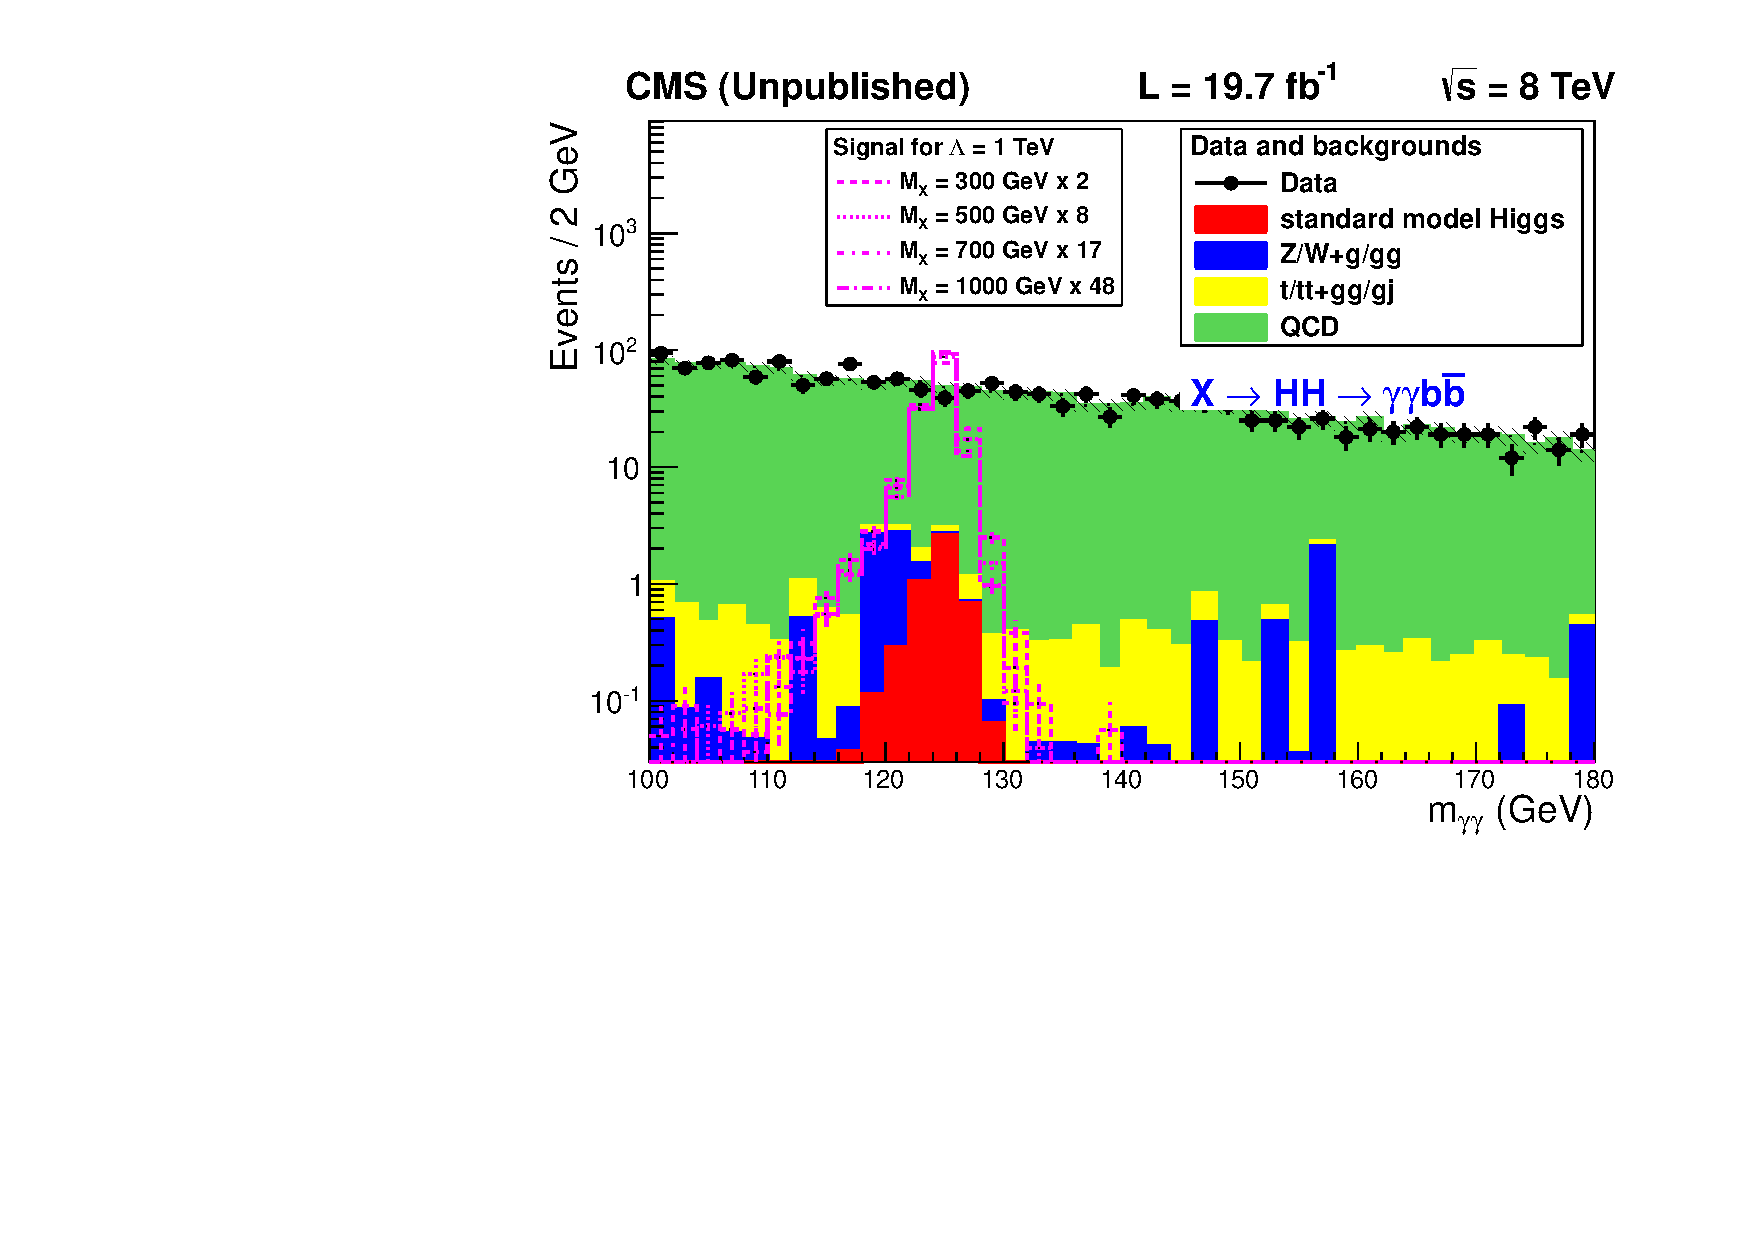
\includegraphics[width=0.70\textwidth]{figures/objects/DiPhotonMass_ShapeNormalized_Log_sys.pdf}
 \end{center}
\caption{Control plots for the diphoton mass spectrum after basic photon and jet selections
and requiring at least one loose b-tagged jet. The simulation is normalized to data and
the statistical uncertainty on the number of simulated events is shown in dashed overlay.
The top (bottom) figure is shown in linear (log) scale.}
\label{fig:mgg_controlplot}
\end{figure}

\section{Jets\label{sec:jets}}

PF jet reconstruction involves the clustering of all PF candidates except the two photons selected
as the $\Hgg$ candidate~\cite{PFPAS2009,CMS-PAS-PFT-10-001}.
The anti-$k_{\rm T}$ algorithm~\cite{Cacciari:2008gp} with a distance parameter of $R = 0.5$ is
used to cluster the PF candidates into jets as an approximate attempt to reverse engineer the
processes of hadronization and fragmentation after a b-quark was produced in the interaction.
In this greedy algorithm, a list of particles and pseudojets is maintained, and at each iteration
elements $i$ and $j$ are combined into one pseudojet if that pair has the minimum distance measure
in the list, where the distance measure $d_{ij}$ is defined as
\begin{equation}
d_{i,j} = \min \left(\frac{1}{k_{{\rm T},i}^2},\frac{1}{k_{{\rm T},j}^2}\right)\frac{\Delta R_{i,j}^2}{R^2} \, ,
\end{equation}
where $k_{{\rm T},i}$ is the transverse momentum of $i$ and $\Delta R_{i,j} = \sqrt{(\eta_i-\eta_j)^2+(\phi_i-\phi_j)^2}$ is the angular separation between $i$ and $j$. If, on a particular iteration,
$d_{i,B}$ is the minimum, defined as
\begin{equation}
d_{i,B} = \frac{1}{k_{{\rm T},i}^2} \, ,
\end{equation}
then element $i$ is considered a jet and is removed from the list. The algorithm continues until the
list is empty.
The advantages of this clustering algorithm is that harder jets tend to be reconstructed as circles
in the $\eta\phi$-plane and that the clustering is not sensitive to hadronization from pileup and the
underlying event.

After the jet reconstruction, the energy is corrected for pileup contributions from both the same
bunch crossing and neighboring bunch crossings. This is accomplished with the the
jet area technique~\cite{Cacciari:2007fd} carried out by the FastJet package~\cite{Cacciari:2011ma}
in which the jet $p_{\rm T}$ is corrected per unit area based on an event-by-event estimation of pileup
activity.
Jet energy is further corrected as a function of the jet $p_{\rm T}$ and $\eta$~\cite{JINST6}
due to potential mismeasurement and the presence of neutrinos.

Additional requirements are imposed to reject jets that originate from detector noise or from the
clustering of particles due to pileup in favor of those that originate from a parton in the
primary interaction~\cite{CMS-PAS-JME-13-005}. Two criteria used are based on the fraction
of charged PF candidates attached to the primary vertex $\beta^*$ and the jet width
$\langle\Delta R^2\rangle$, defined as
\begin{subequations}
\begin{equation}
\beta^* = \frac{\sum_{i\in \text{other PV}} p_{{\rm T},i}}{\sum_{i\in\text{charged}} p_{{\rm T},i}}
\end{equation}
\begin{equation}
\langle\Delta R^2\rangle = \frac{\sum_i \Delta R_i^2 p_{{\rm T},i}^2}{\sum_i p_{{\rm T},i}^2} \, ,
\end{equation}
\end{subequations}
where ``other PV'' refers to the PF charged candidates associated to another primary vertex, the sum
in the denominator of $\beta^*$ is over the charged candidates in the jet, the sums
in $\langle\Delta R^2\rangle$ are over all constituents in the jet, and $\Delta R_i$ is the
angular distance between constituent $i$ and the jet axis. Upper thresholds are imposed on these
quantities; in the case of $\beta^*$ the threshold is a function of the number of reconstructed
vertices.

The efficiency of the jet identification from the above criteria exceeds 95\%. Additional kinematic
requirements on the jets include $p_{\rm T} > 25$~GeV and $|\eta| < 2.5$ (within the tracker
acceptance). In the case that more than two jets pass identification and kinematic selections, the
two jets with the highest $p_{{\rm T},jj}$ are chosen to make the dijet candidate, which will
be discussed in more detail in Section~\ref{sec:higgsreconstruction}.
Figure~\ref{fig:mjj_onlyhiggs} shows the resulting simulated distributions for the
dijet mass of the resonant signal and resonant backgrounds.
Figure~\ref{fig:mjj_controlplot} shows the same
distribution for data and the sum of backgrounds. (Note that these figures include a requirement
on the compatibility of one of the jets coming from a b-quark, discussed in Section~\ref{subsec:btag}.)


\begin{figure}[ht]
 \begin{center}
    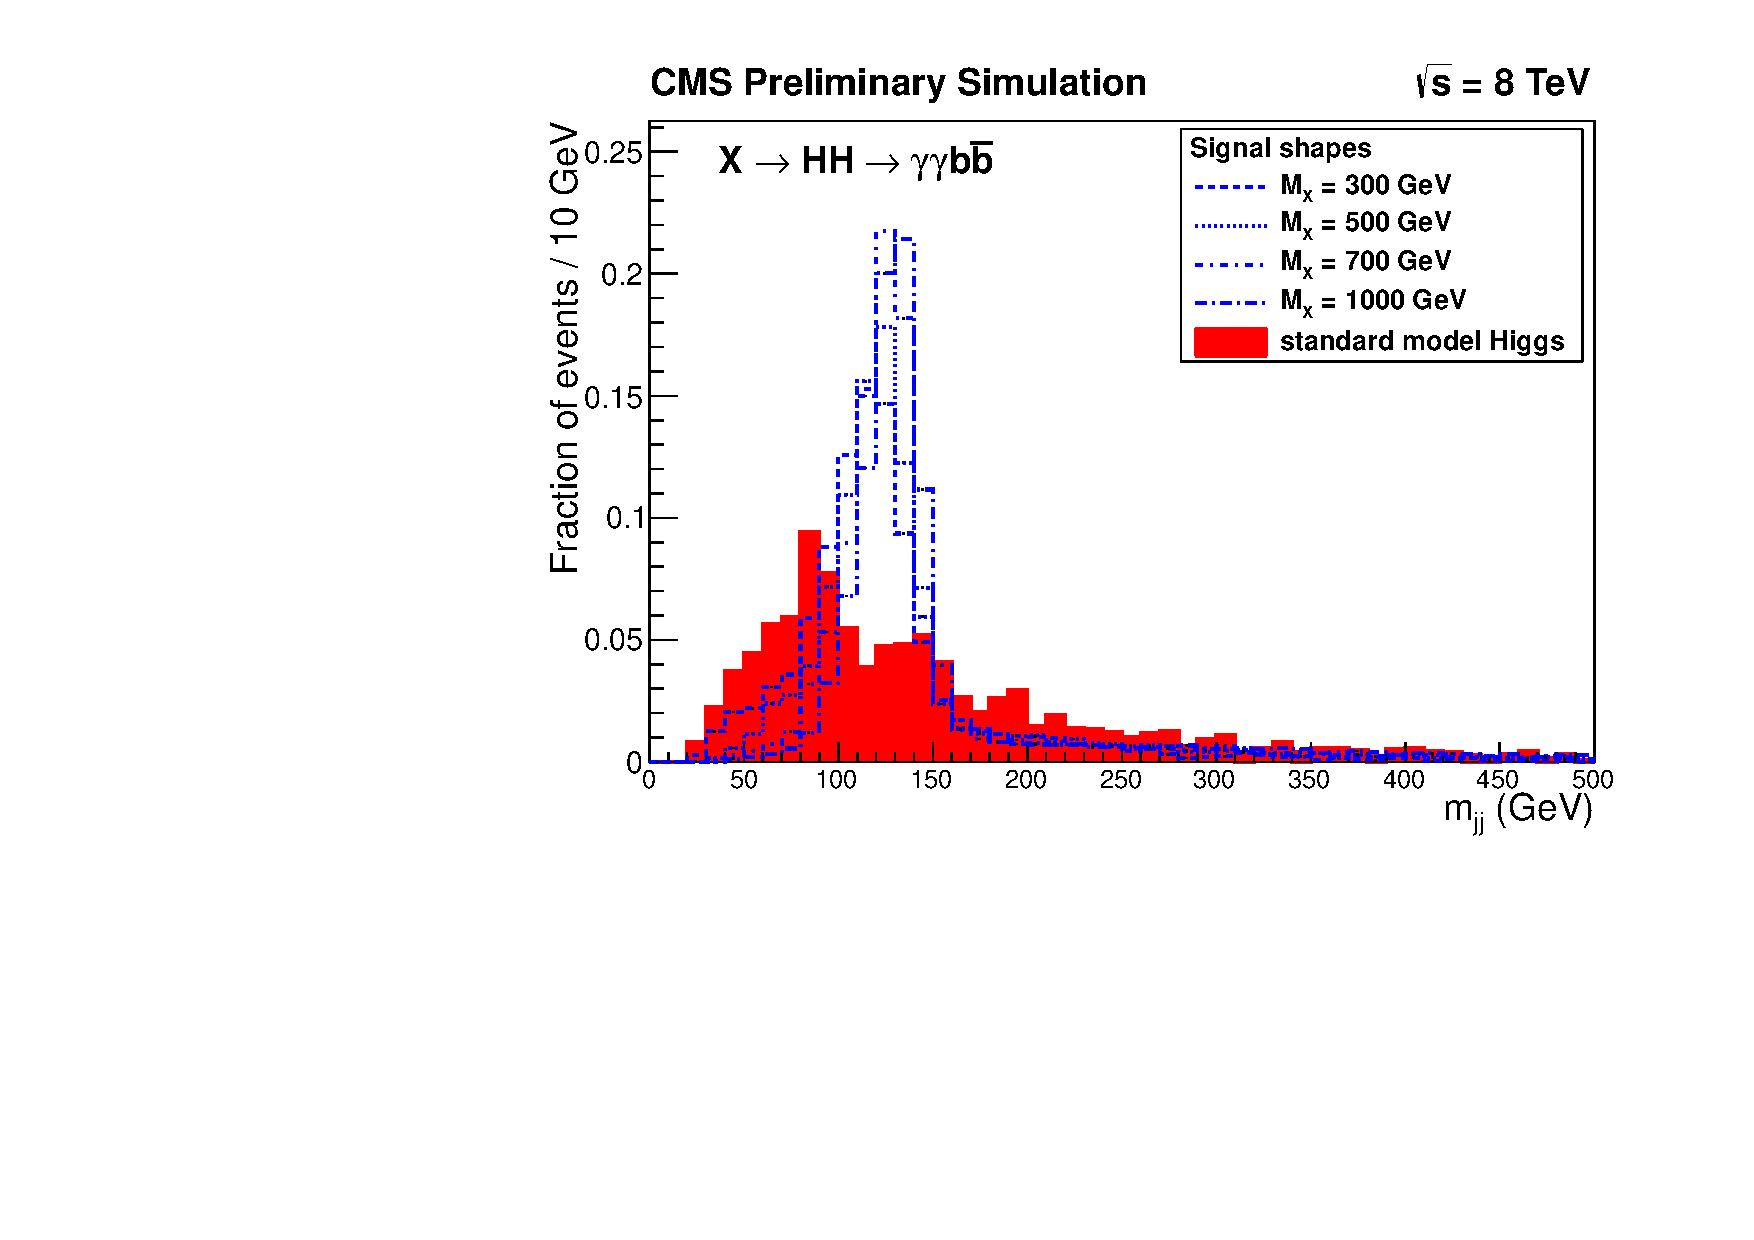
\includegraphics[width=0.70\textwidth]{figures/objects/DiJetMass_OnlyHiggs.pdf}
 \end{center}
\caption{Simulated dijet mass spectrum for the resonant signal and the sum of all production
mechanisms of the
SM Higgs boson after basic selections on photons and jets and requesting at least one loose
b-tagged jet.
The spectra are normalized to one.}
\label{fig:mjj_onlyhiggs}
\end{figure}

\begin{figure}[ht]
 \begin{center}
   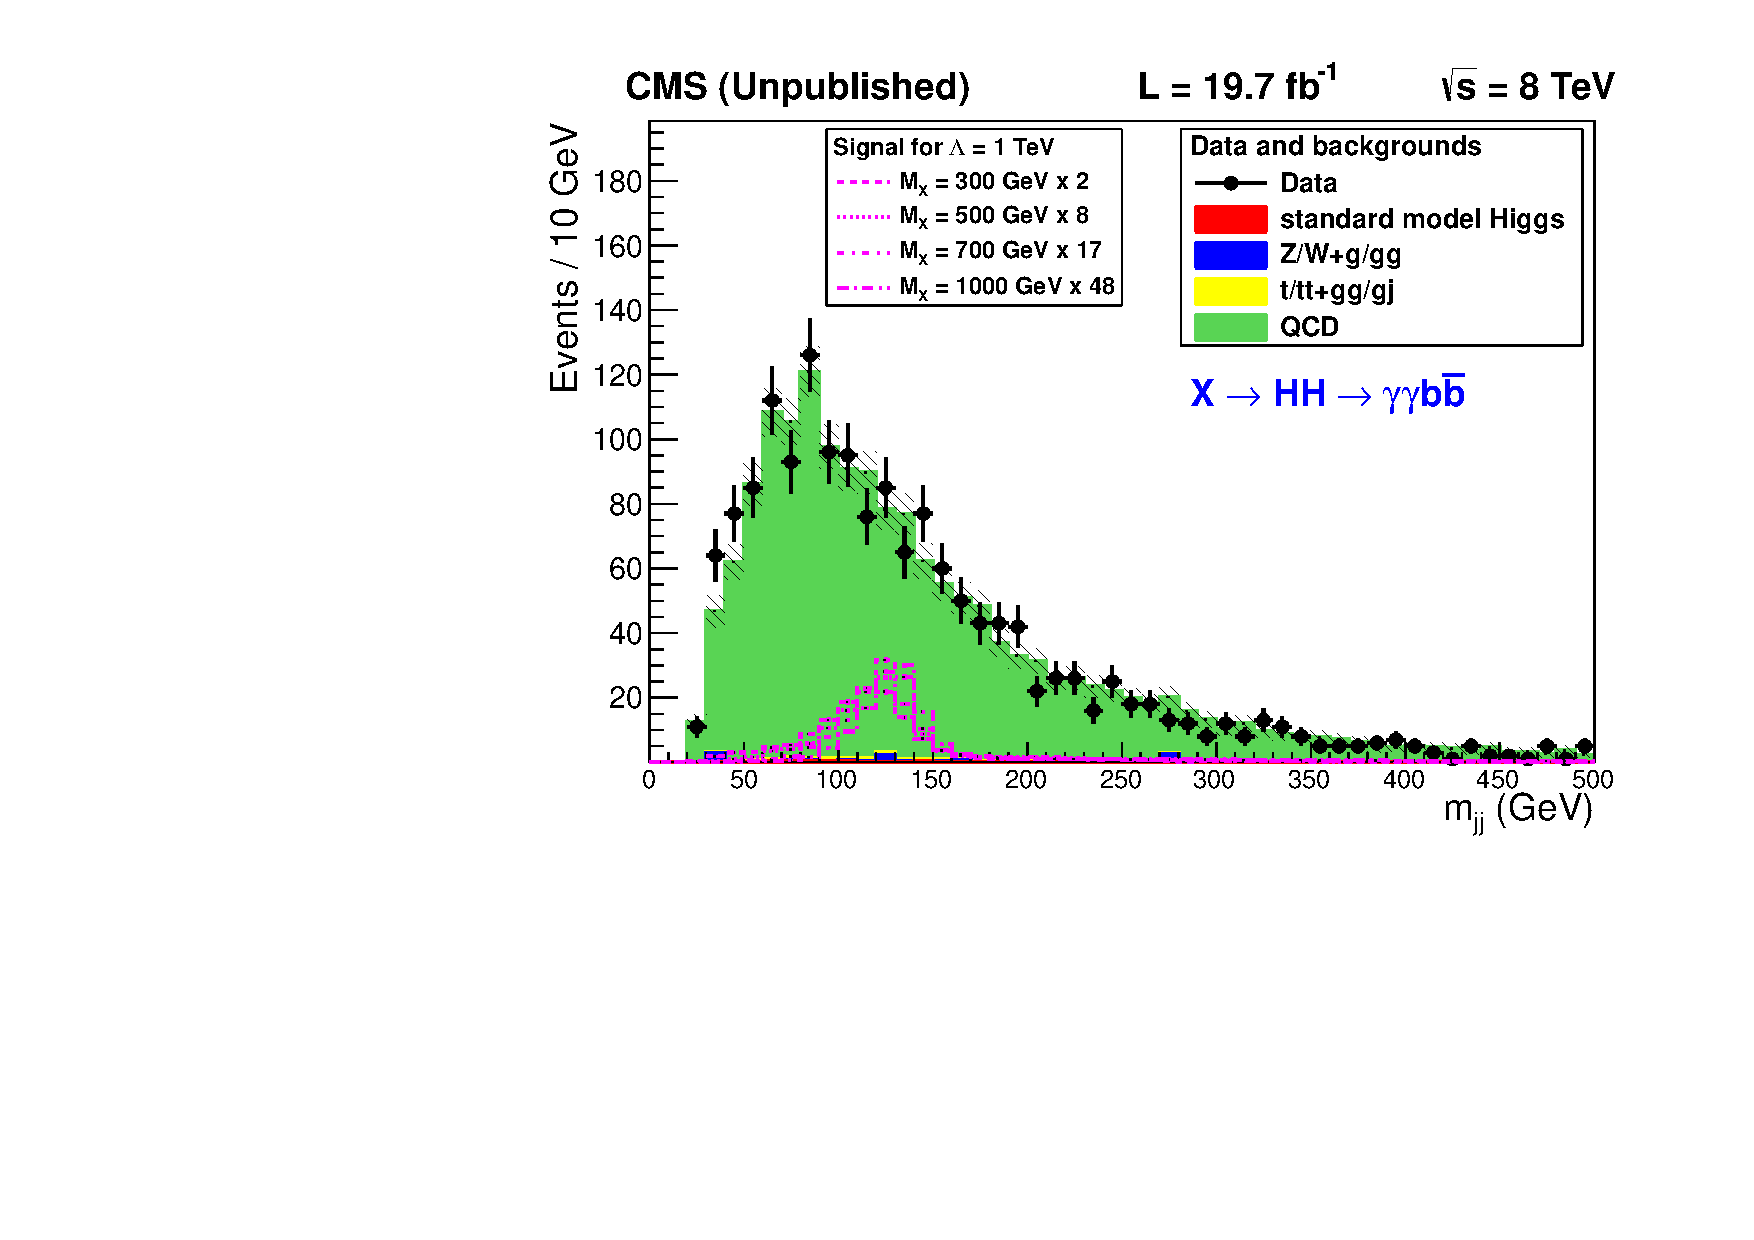
\includegraphics[width=0.70\textwidth]{figures/objects/DiJetMass_ShapeNormalized_sys.pdf}
   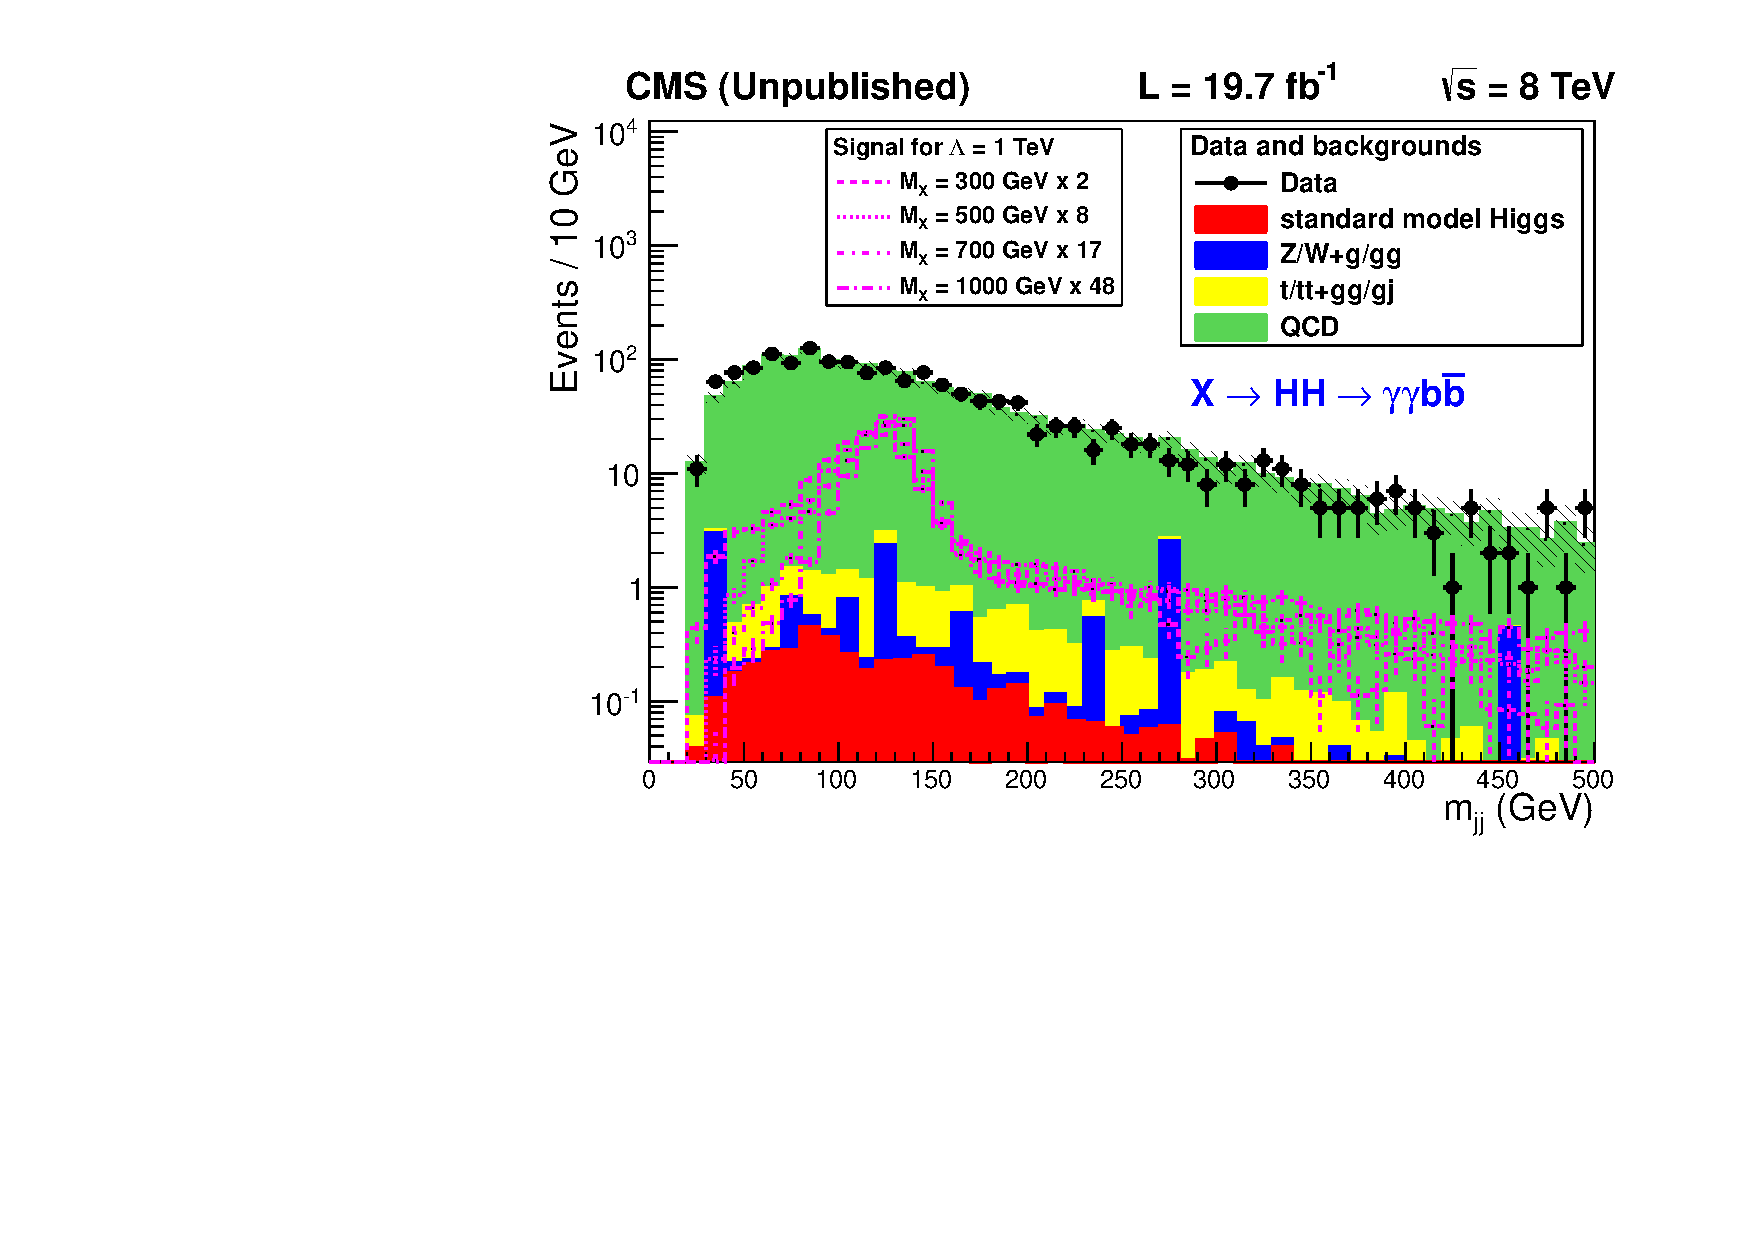
\includegraphics[width=0.70\textwidth]{figures/objects/DiJetMass_ShapeNormalized_Log_sys.pdf}
 \end{center}
\caption{Control plots for the dijet mass spectrum after basic photon and jet selections
and requiring at least one loose b-tagged jet. The simulation is normalized to data and
the statistical uncertainty on the number of simulated events is shown in dashed overlay.
The top (bottom) figure is shown in linear (log) scale.}
\label{fig:mjj_controlplot}
\end{figure}

\subsection{B-tagging\label{subsec:btag}}

The relatively long lifetime of B mesons, coming from the production of a b-quark in the event,
means that these mesons travel around $500~\mu m$ on average before decaying into more stable
light-flavor hadrons.
This property is exploited by looking for tracks consistent with a secondary vertex from
the B-meson decay and allows for further discrimination between signal and background events.
The Combined Secondary Vertex (CSV) b-tagger~\cite{BTV} combines
information from track impact parameters and secondary vertices within a given jet, and
provides a continuous output which provides discrimination between jets coming from the
hadronization of a b-quark against light-flavor and gluon jets.
The efficiency to tag b-jets and the rate of misidentification depends on the chosen threshold
of the CSV output and are measured in data samples enriched in b-jets, for example in $t\bar{t}$ events.
The simulation samples are corrected by applying event weights to account for the
differences between data and simulation with respect to the b-tag efficiency.
At preselection level, one loose b-tagged jet (CSVL) is required in the event, which corresponds to
a mistag rate of 10\%.

\subsection{Jet Energy Regression}

The jet energy corrections are performed globally on average for all jets, whereas the jets in
the signal of interest originate from the hadronization of b-quarks. Therefore, the correction
can be improved by exploiting the properties of these jets, which will in turn improve the resolution
of the dijet mass. A motivation for implementing an additional correction is to improve separation
between signal and background, particularly against
the resonance background $Z(b\bar{b})H(\gamma\gamma)$,
since the mass of the Z is very close to that of the Higgs relative to the dijet mass resolution.

Here a jet energy regression is presented, which acts as a multidimensional calibration tuned to the
specific jet properties of the signal. It is not used in the final analysis, but it can serve
as a 10--20\% improvement in sensitivity of the low-mass resonant signal
for future iterations of the analysis.

The correction comes from training a Boosted Decision Tree (BDT) regression simultaneously
on half of the MSSM signal
samples at resonant masses of 260, 300, and 350 GeV; these samples were previously
discussed in Section~\ref{subsec:sig_samples}.
These samples are generated with about 50k events each and are independent of the Radion
samples on which the final limits are extracted.

The regression is trained on every jet passing the identification criterion and the
following kinematic criteria:
\begin{itemize}
\item $p_T > 20$~GeV,
\item $|\eta|<2.5$, and
\item $\Delta R (j, j_\text{gen}) < 0.4$ (the angular separation between the jet and its associated
generator-level jet).
\end{itemize}                                                                                           
The $p_T$ threshold is increased to 25 GeV for testing and implementation.

The BDT algorithm is implemented from the TMVA package~\cite{TMVA2007} using gradient boost.
The input variables are
\begin{itemize}
\item the jet transverse momentum $p_T$,
\item the jet transverse mass $m_T$,
\item the jet pseudorapidity $\eta$,
\item the jet PF photon energy fraction,
\item the jet PF neutral hadron energy fraction,
\item the number of PF jet constituents (both charged and neutral),
\item the lead track $p_T$ associated to the jet,
\item the jet secondary vertex flight distance error (if there is a secondary vertex),
\item the jet secondary vertex mass (if there is a secondary vertex),
\item the soft lepton $p_T$ (if there is a soft lepton in the jet),
\item the soft lepton relative $p_T$ in direction of the jet (if there is a soft lepton in the jet),
\item PF $\met$ with $\Hgg$ specific corrections~\cite{HggCMS},
\item $\Delta \phi (j, \met)$, and
\item the median jet energy per jet area $\rho$. 
\end{itemize}
The secondary vertex refers to that of the B-meson decay, if such a vertex was identified.
The soft lepton refers to an electron or muon resonstructed inside the cone of the jet.

The figure of merit to quantify the effect of the regression is the resolution improvements
measured in the dijet and four-body ($\ggjj$) mass spectra of the signal sample.
Possible overtraining has been studied and considered negligible.
The resolution improvements in the \Mjj\, and \Mggjj\, spectra are quoted through a
fit to each spectrum using the sum of a Crystal Ball and third-order polynomial for events
in both 1-tag and 2-tag categories, which will be discussed in Section~\ref{sec:classification}.
The parameters of the Crystal Ball give estimates
of the spread and central value of the distribution, and the ratio of these two gives the resolution.
Table~\ref{table:regression_improvement_res} shows in improvement in the resolution separately
for the two spectra and for the two event categories.
The improvement is shown visually in the $\Mjj$ spectrum in
Figure~\ref{fig:regression_plots_improvement_mjj} where both event categories are combined.

\begin{table}[ht]
  \centering
  \renewcommand{\arraystretch}{1.4}
  \caption{Improvement from the regression on $\Mggjj$ and $\Mjj$ spectra, divided into 1-tag or 2-tag
categories. (Categorization is discussed in Section~\ref{sec:classification}.)
All numbers are in units of percentage.}
  \begin{tabular}{c||c|c|c|c|}
 & \multicolumn{2}{|c|}{\Mggjj\, spectrum} & \multicolumn{2}{|c|}{\Mjj\, spectrum} \\\hline
$m_X$ (GeV) & 1-tag & 2-tag & 1-tag & 2-tag \\ \hline
270 & 19.72 & 3.10  & 15.08 & 12.24 \\  
300 & 16.64 & 8.70  & 16.05 & 14.19 \\  
350 & 19.76 & 13.62 & 23.07 & 18.95 \\  
400 & 19.82 & 21.23 & 17.03 & 14.74 \\ 
\end{tabular}

  \label{table:regression_improvement_res}
\end{table}

\begin{figure}[ht]
\begin{center}
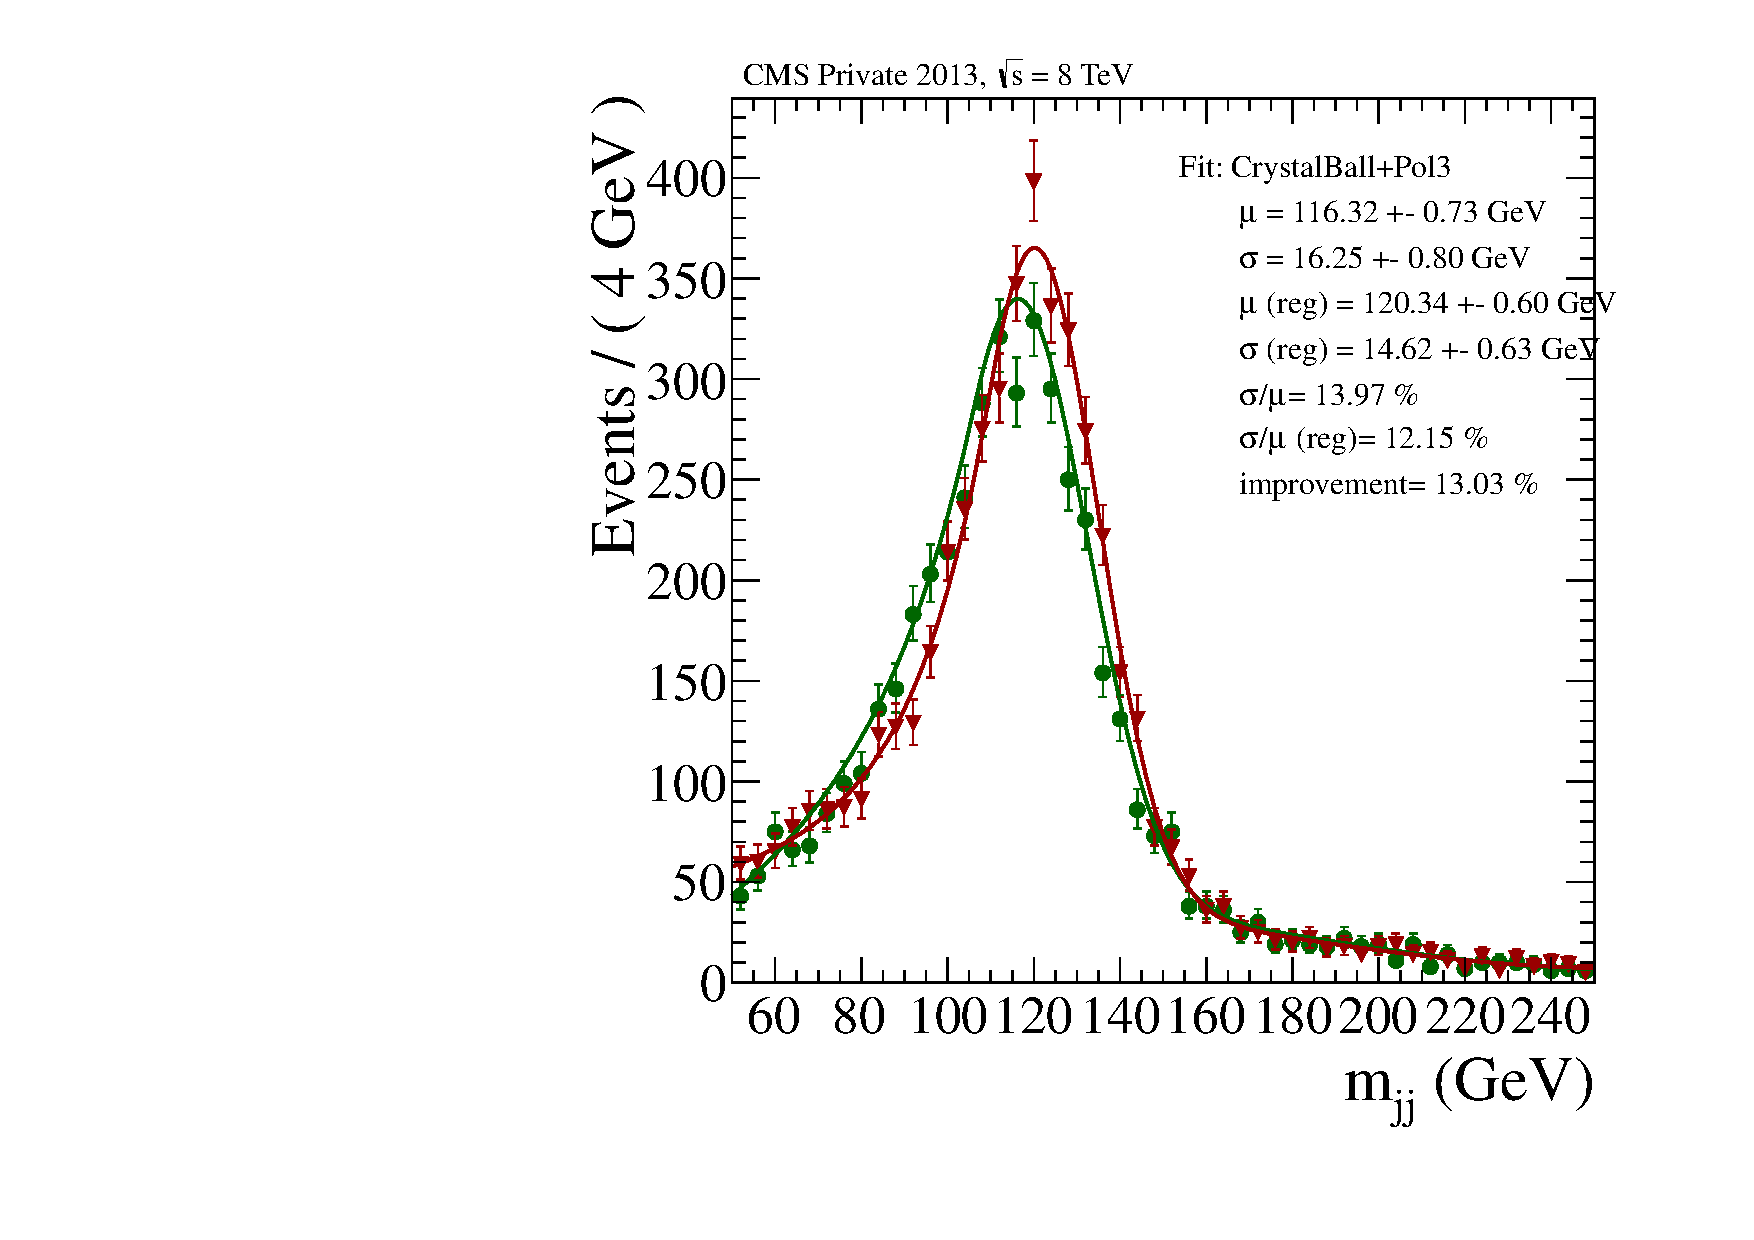
\includegraphics[width=.4\textwidth]{figures/objects/mjj_m270_CrystalBall_allcat.pdf}
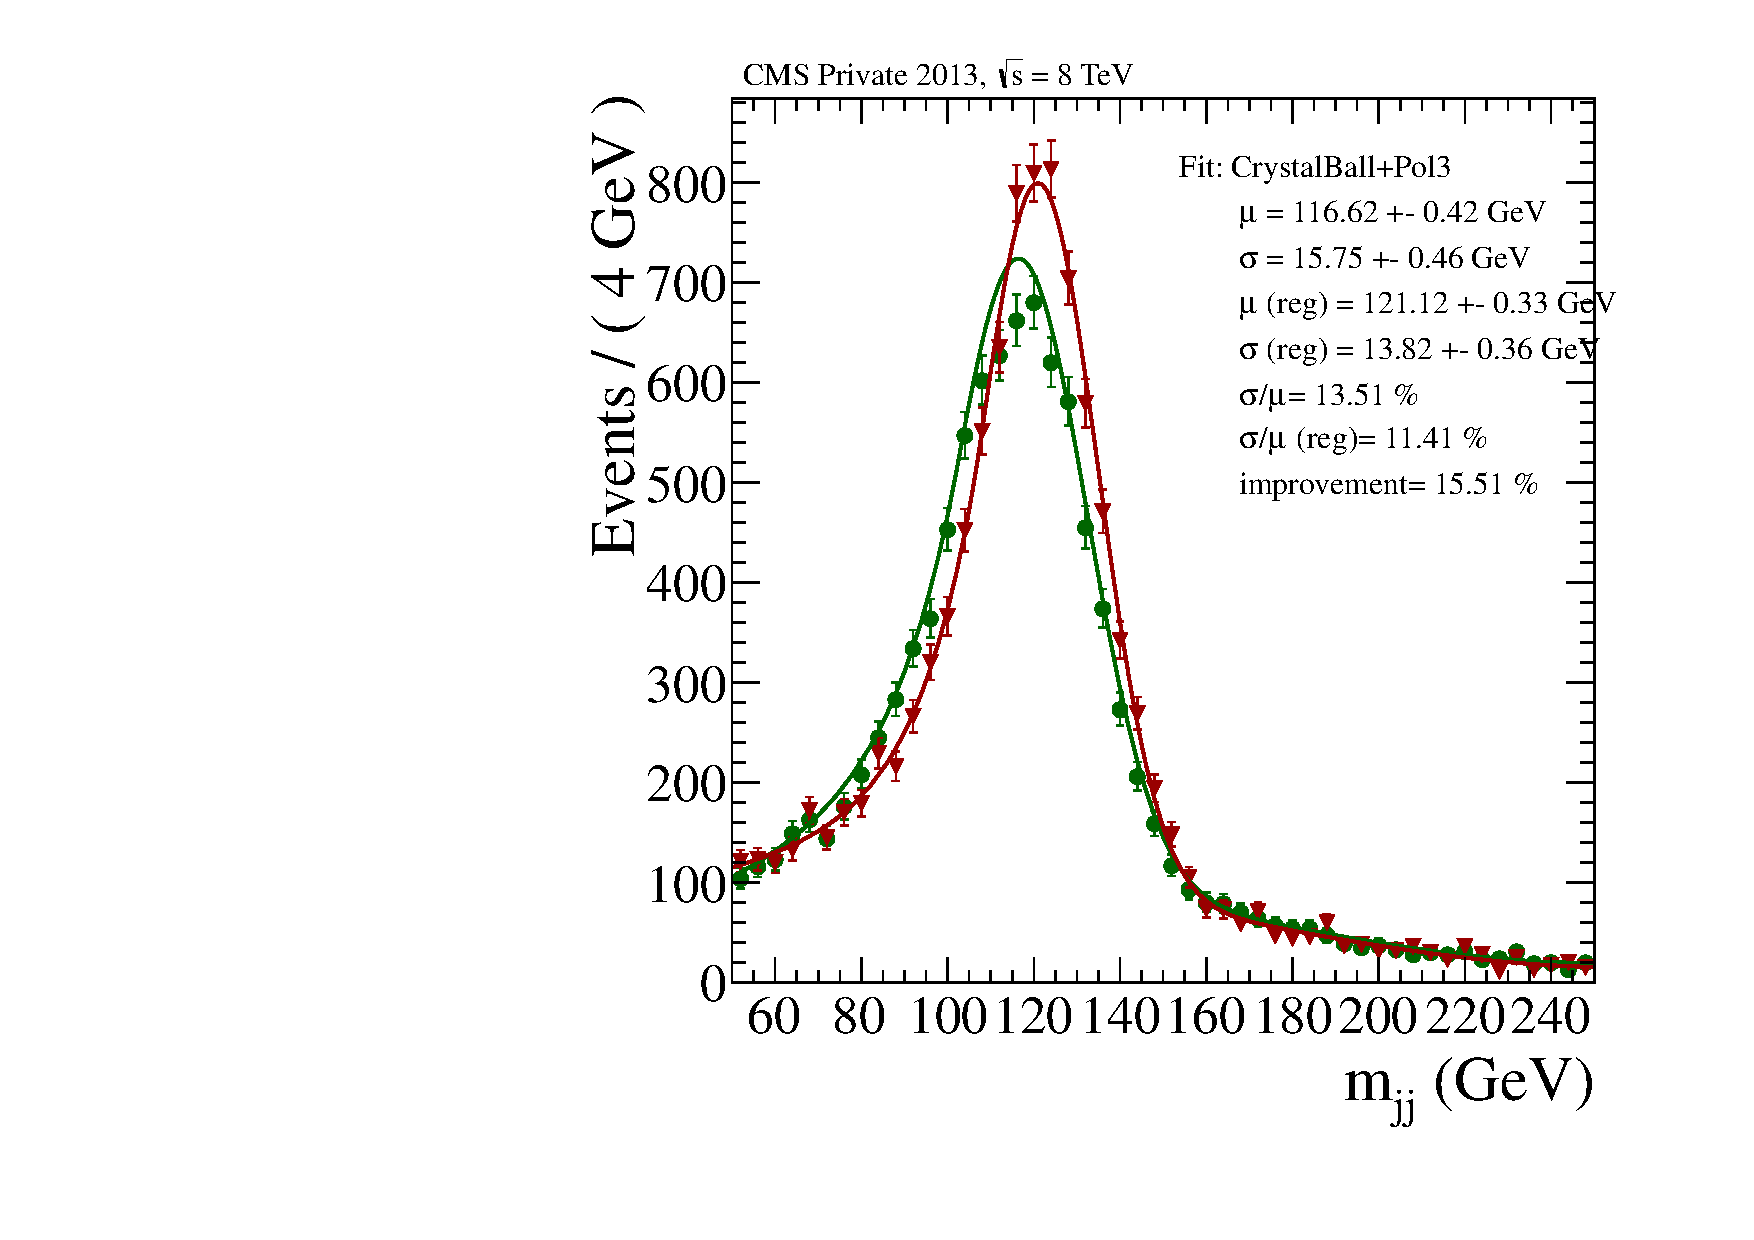
\includegraphics[width=.4\textwidth]{figures/objects/mjj_m300_CrystalBall_allcat.pdf}
\\
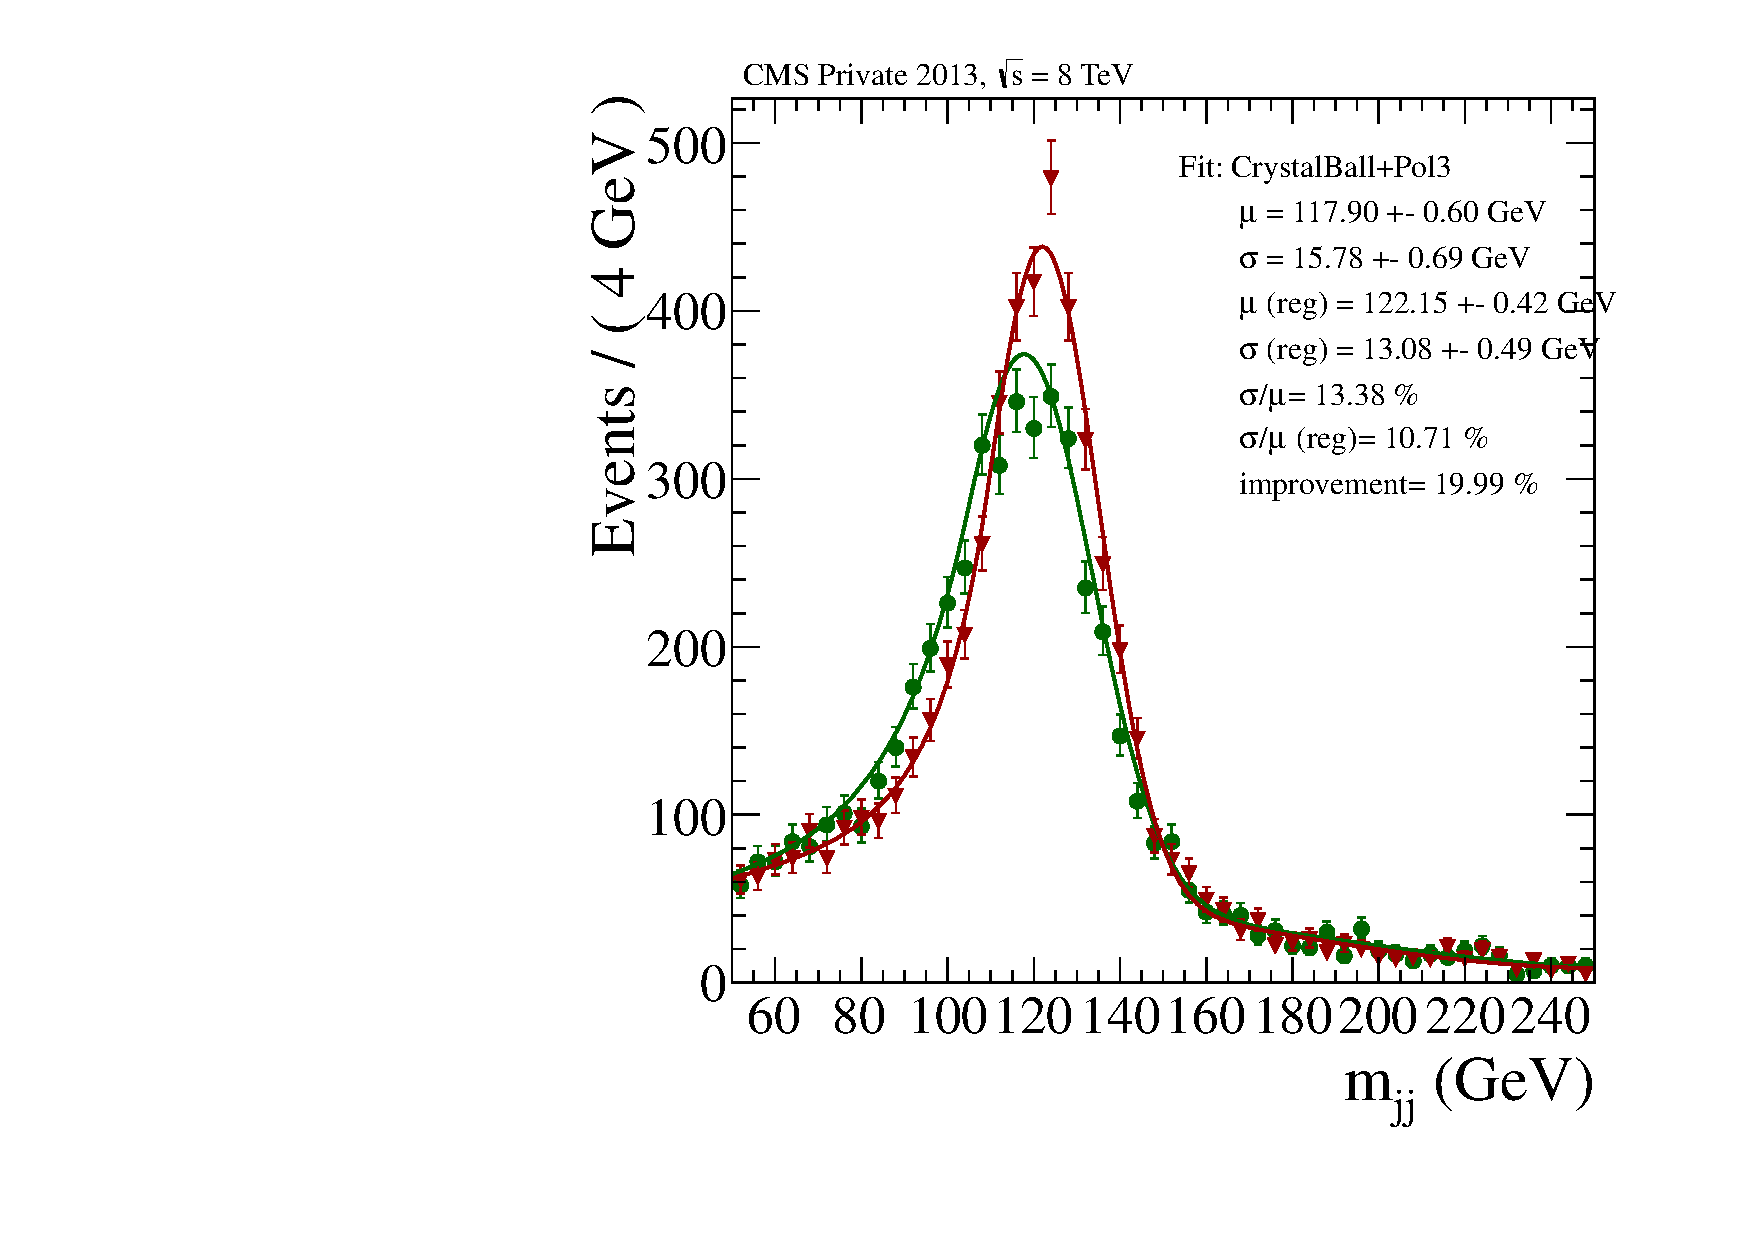
\includegraphics[width=.4\textwidth]{figures/objects/mjj_m350_CrystalBall_allcat.pdf}
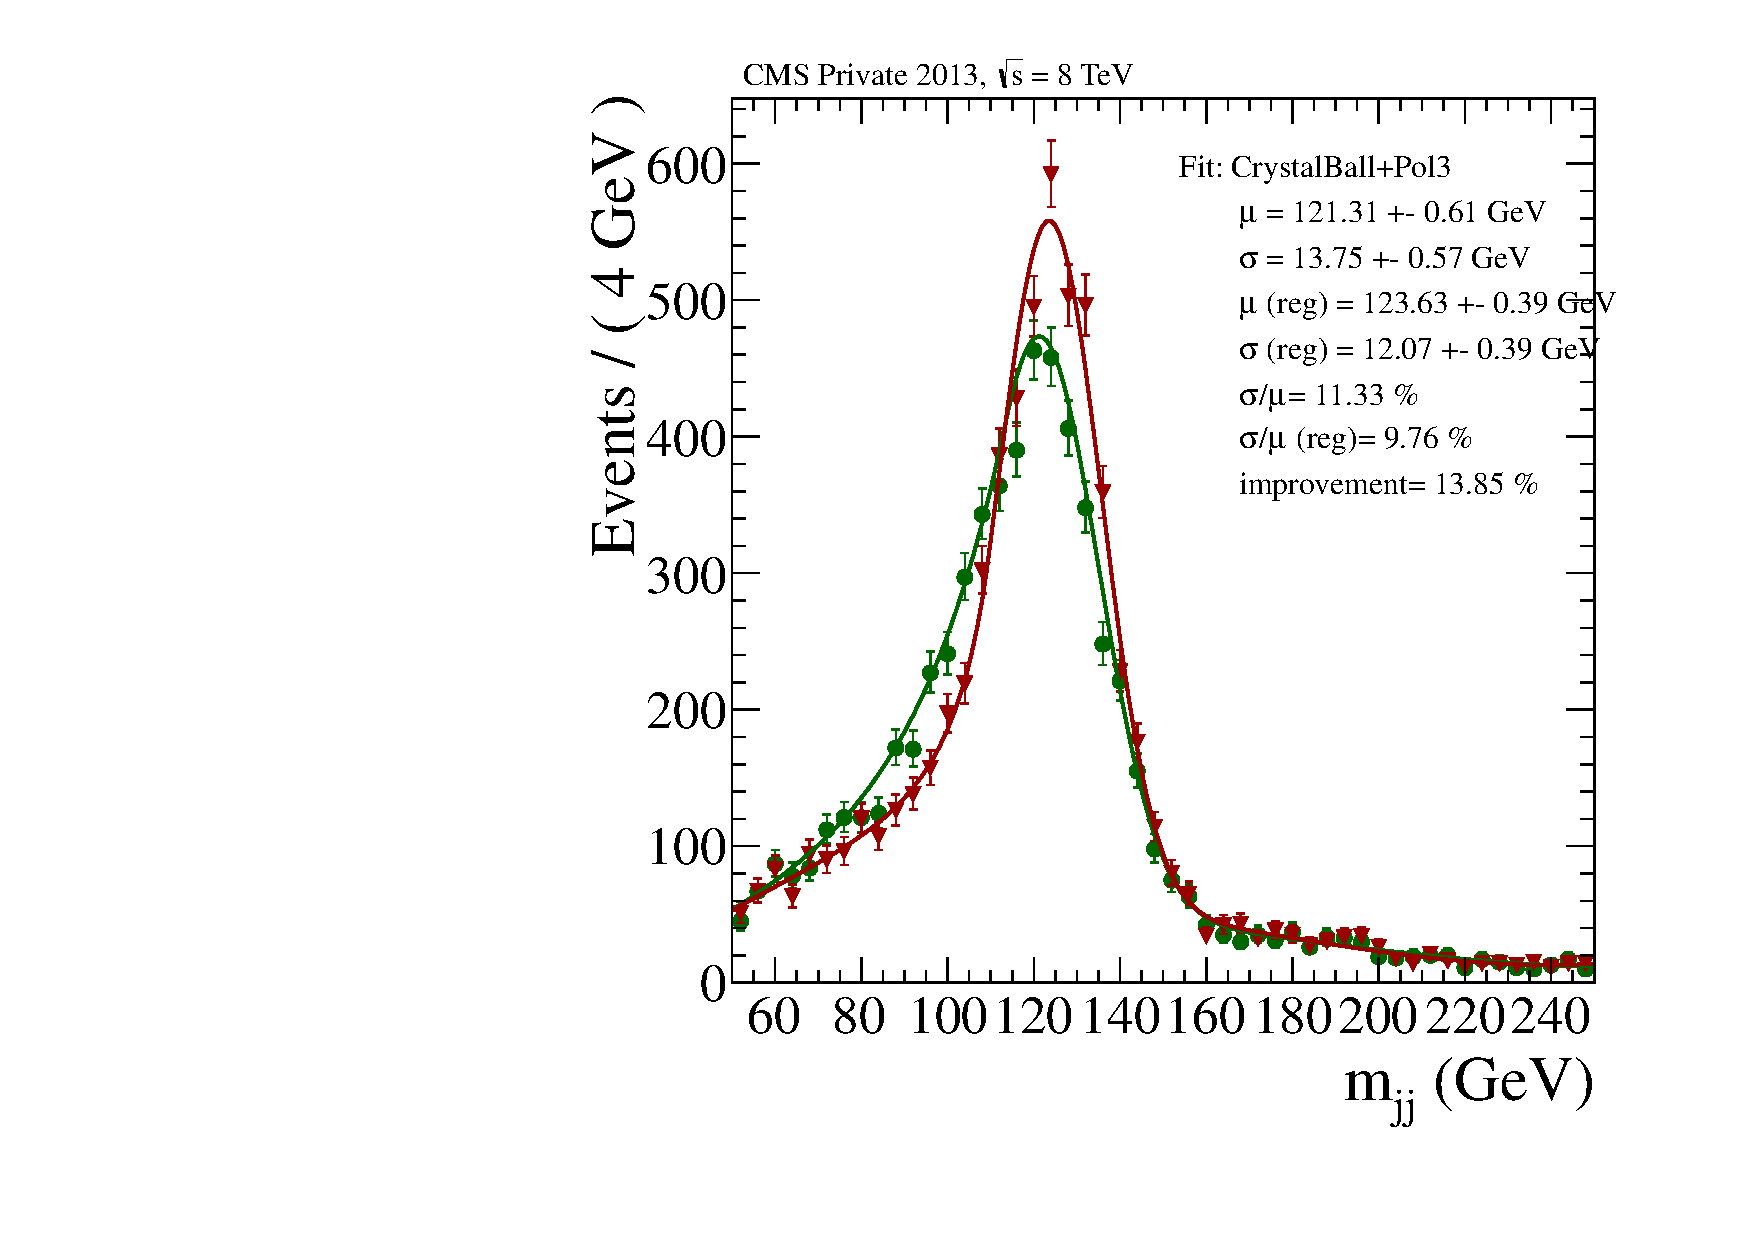
\includegraphics[width=.4\textwidth]{figures/objects/mjj_m400_CrystalBall_allcat.pdf}
\end{center}
\caption{Resolution improvements for the \Mjj\, spectrum at $m_X = 270, 300, 350, 400$~GeV mass points.
The green distribution is before applying the regression, and the red one is after applying the
regression. The fit model is the sum of a Crystal Ball and third-order polynomial.
}
\label{fig:regression_plots_improvement_mjj}
\end{figure}

For validation of the technique, the effect of the regression is studied on data.
Figure~\ref{fig:regression_plots_dataCS_mjj} shows the effect on the data control sample
(a $\gjjj$ sample reweighted to the $\ggjj$ data, discussed in Section~\ref{subsec:dataCS}). The peak
is slightly shifted, and in the region about the Higgs mass, the yield increases about 10\% without
any local peaking structure. 
In addition, comparison between data and the sum of MC backgrounds was performed for the $p_{\rm T}$
balance between the dijet and diphoton candidates before and after regression.
As shown in Figure~\ref{fig:regression_validation_datavsmc}, the ratio
$\frac{p_{{\rm T},jj}}{p_{{\rm T},\gamma\gamma}}$ has peak a more narrow and shifted closer
to 1 after the regression is applied. Although the effect indicates the regression is doing its job,
the data and background processes exhibit a slight overcorrection.

\begin{figure}[ht]
\begin{center}
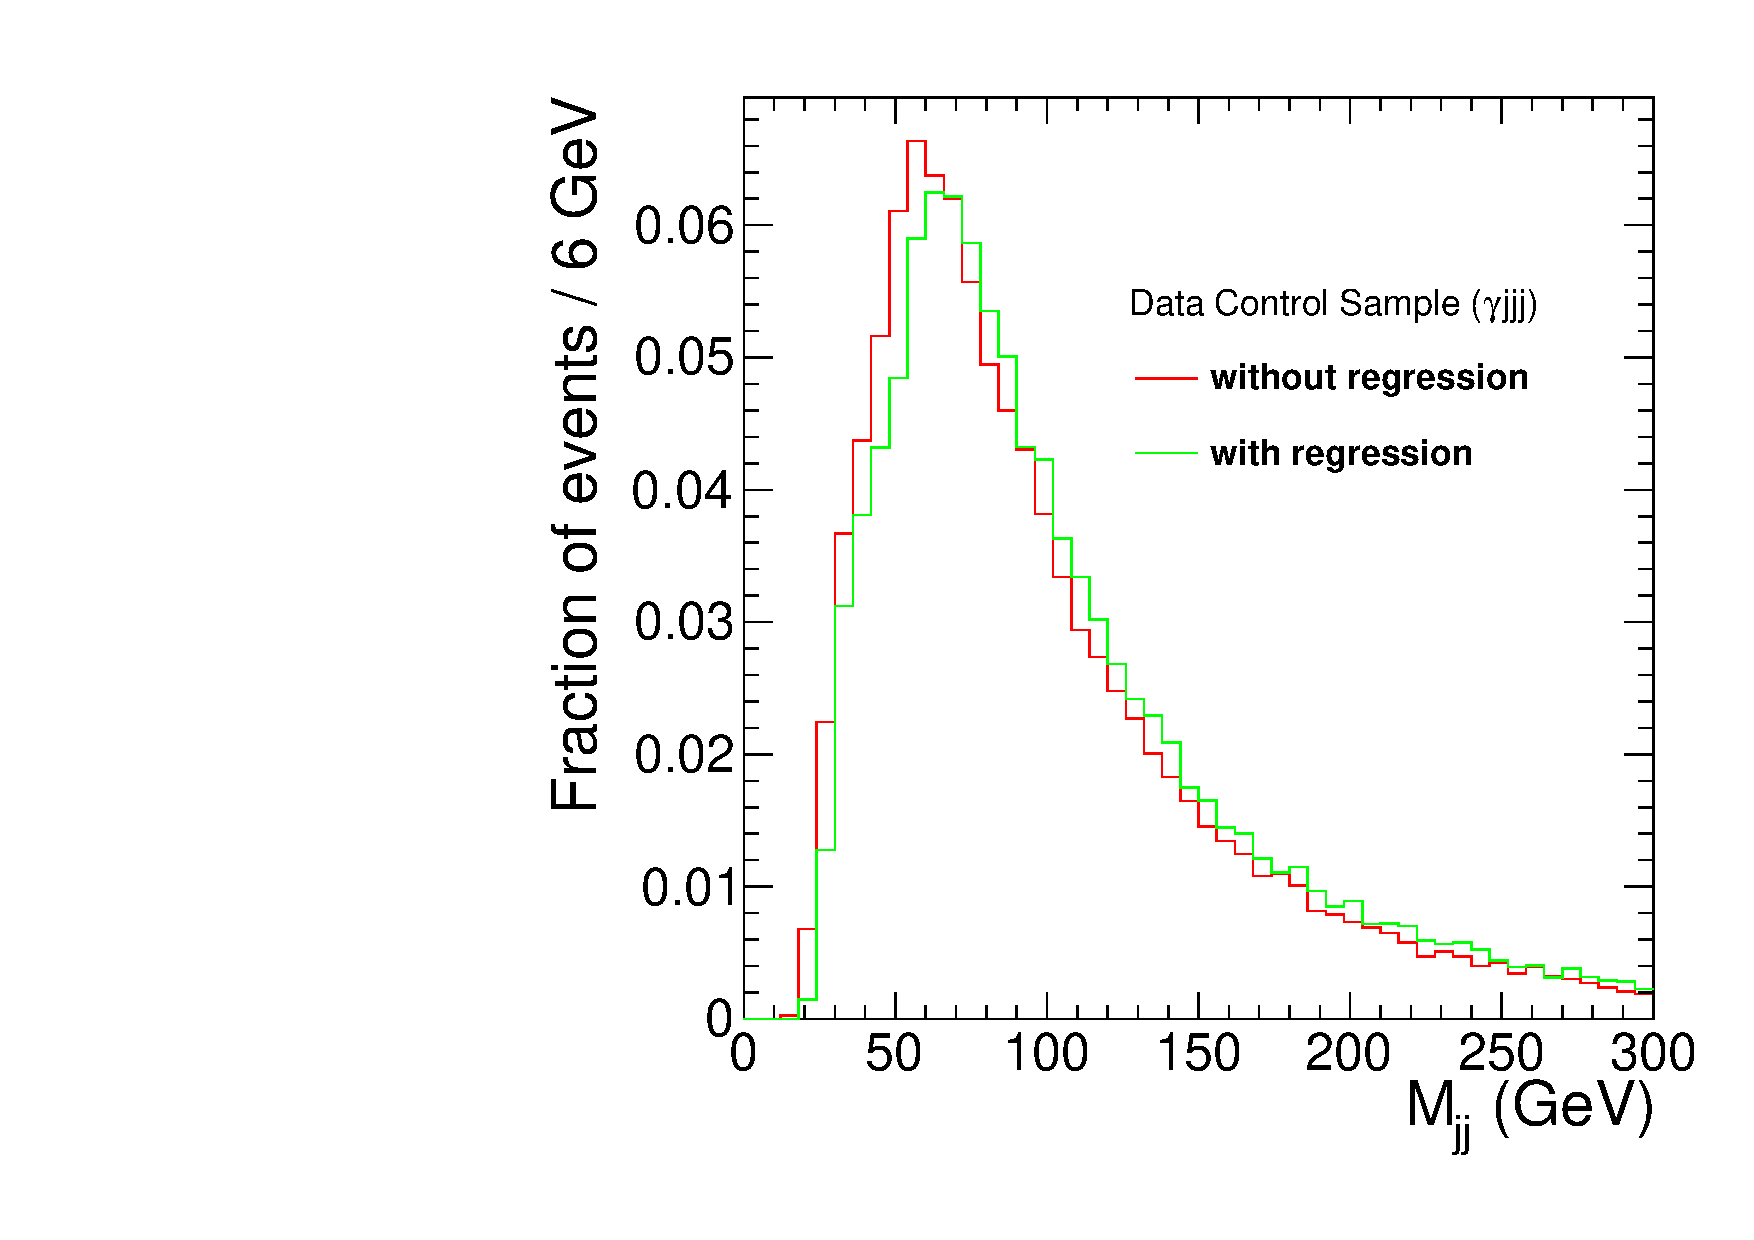
\includegraphics[width=.4\textwidth]{figures/objects/dataCS_mjj.pdf}
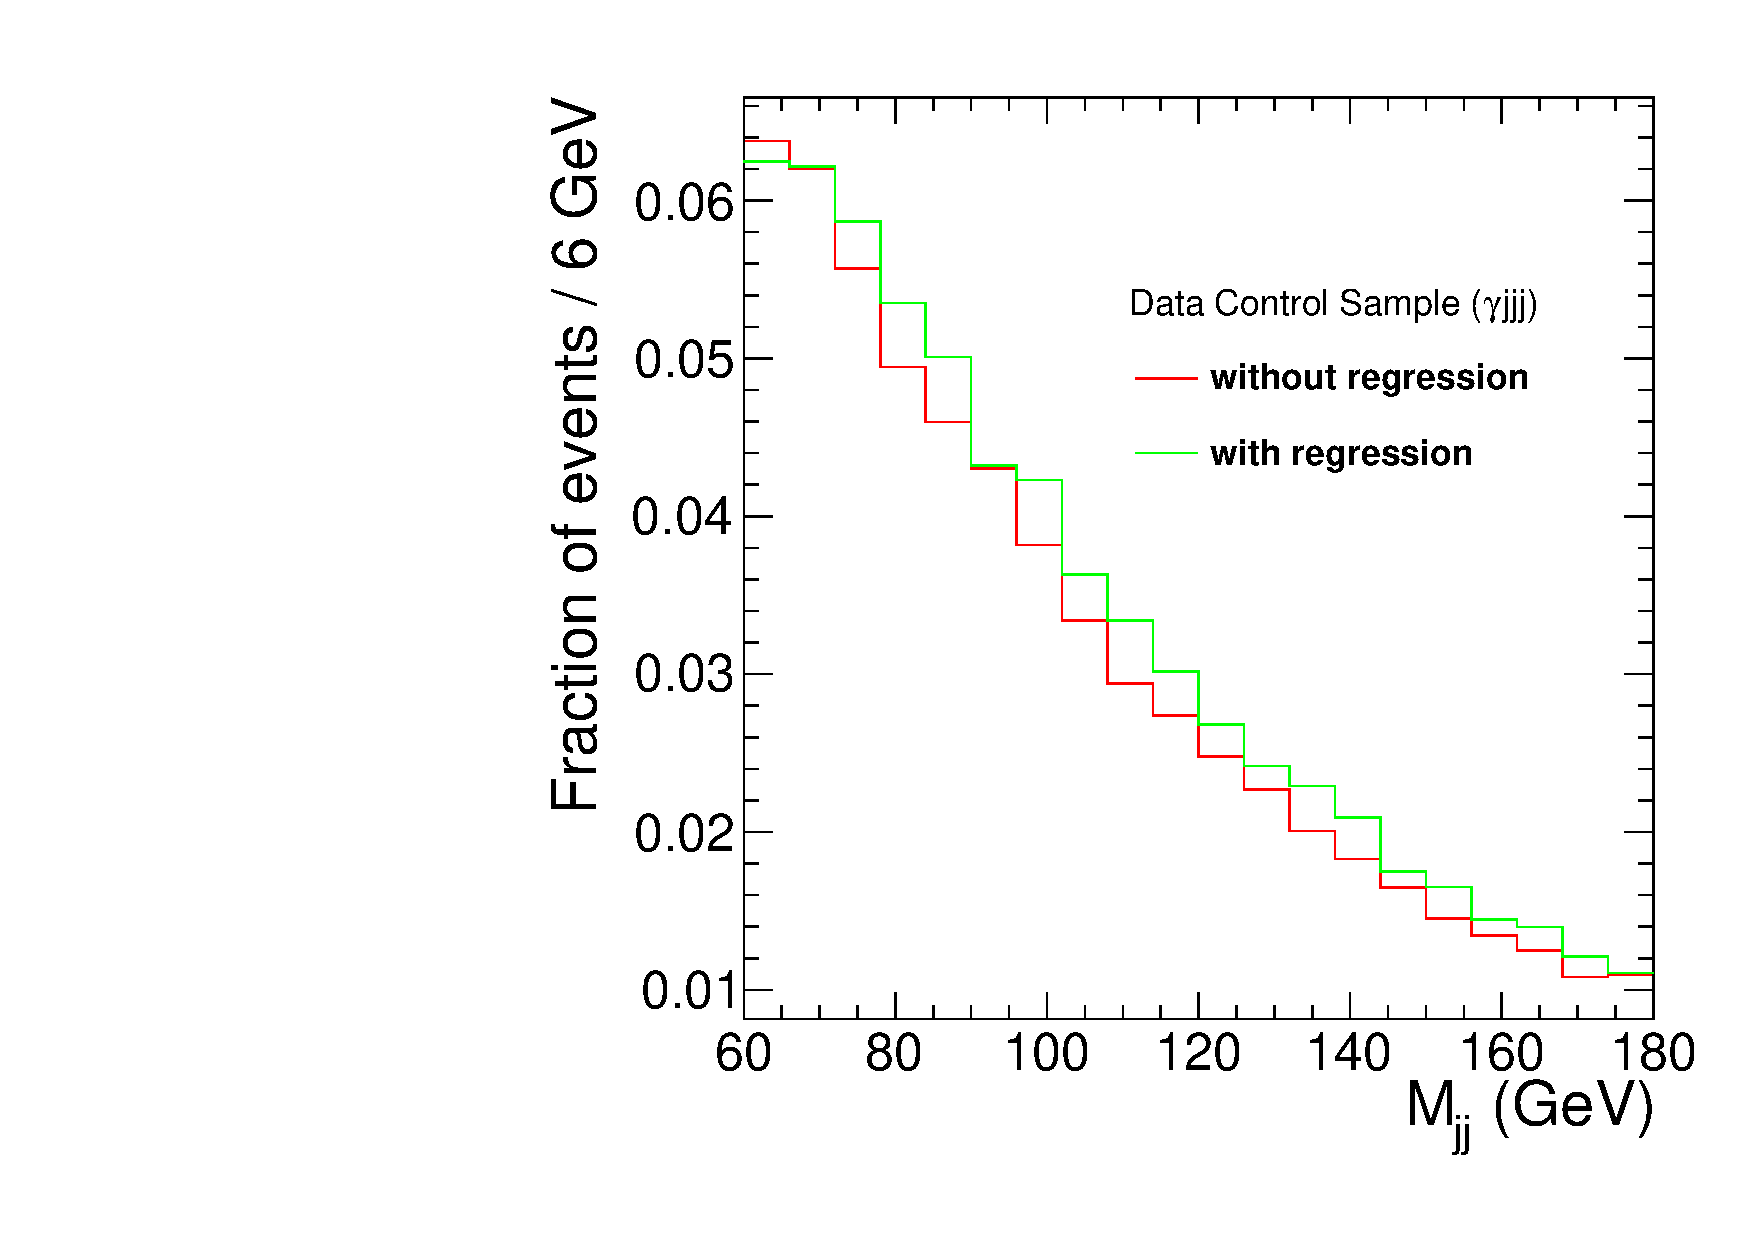
\includegraphics[width=.4\textwidth]{figures/objects/dataCS_mjj_zoom.pdf}
\end{center}
\caption{Effect of regression on the entire \Mjj\, spectrum (left) and zoomed (right)
to a range about the SM Higgs mass on the data control sample, discussed in
Section~\ref{subsec:dataCS}.}
\label{fig:regression_plots_dataCS_mjj} 
\end{figure}

\begin{figure}[ht]
\begin{center}
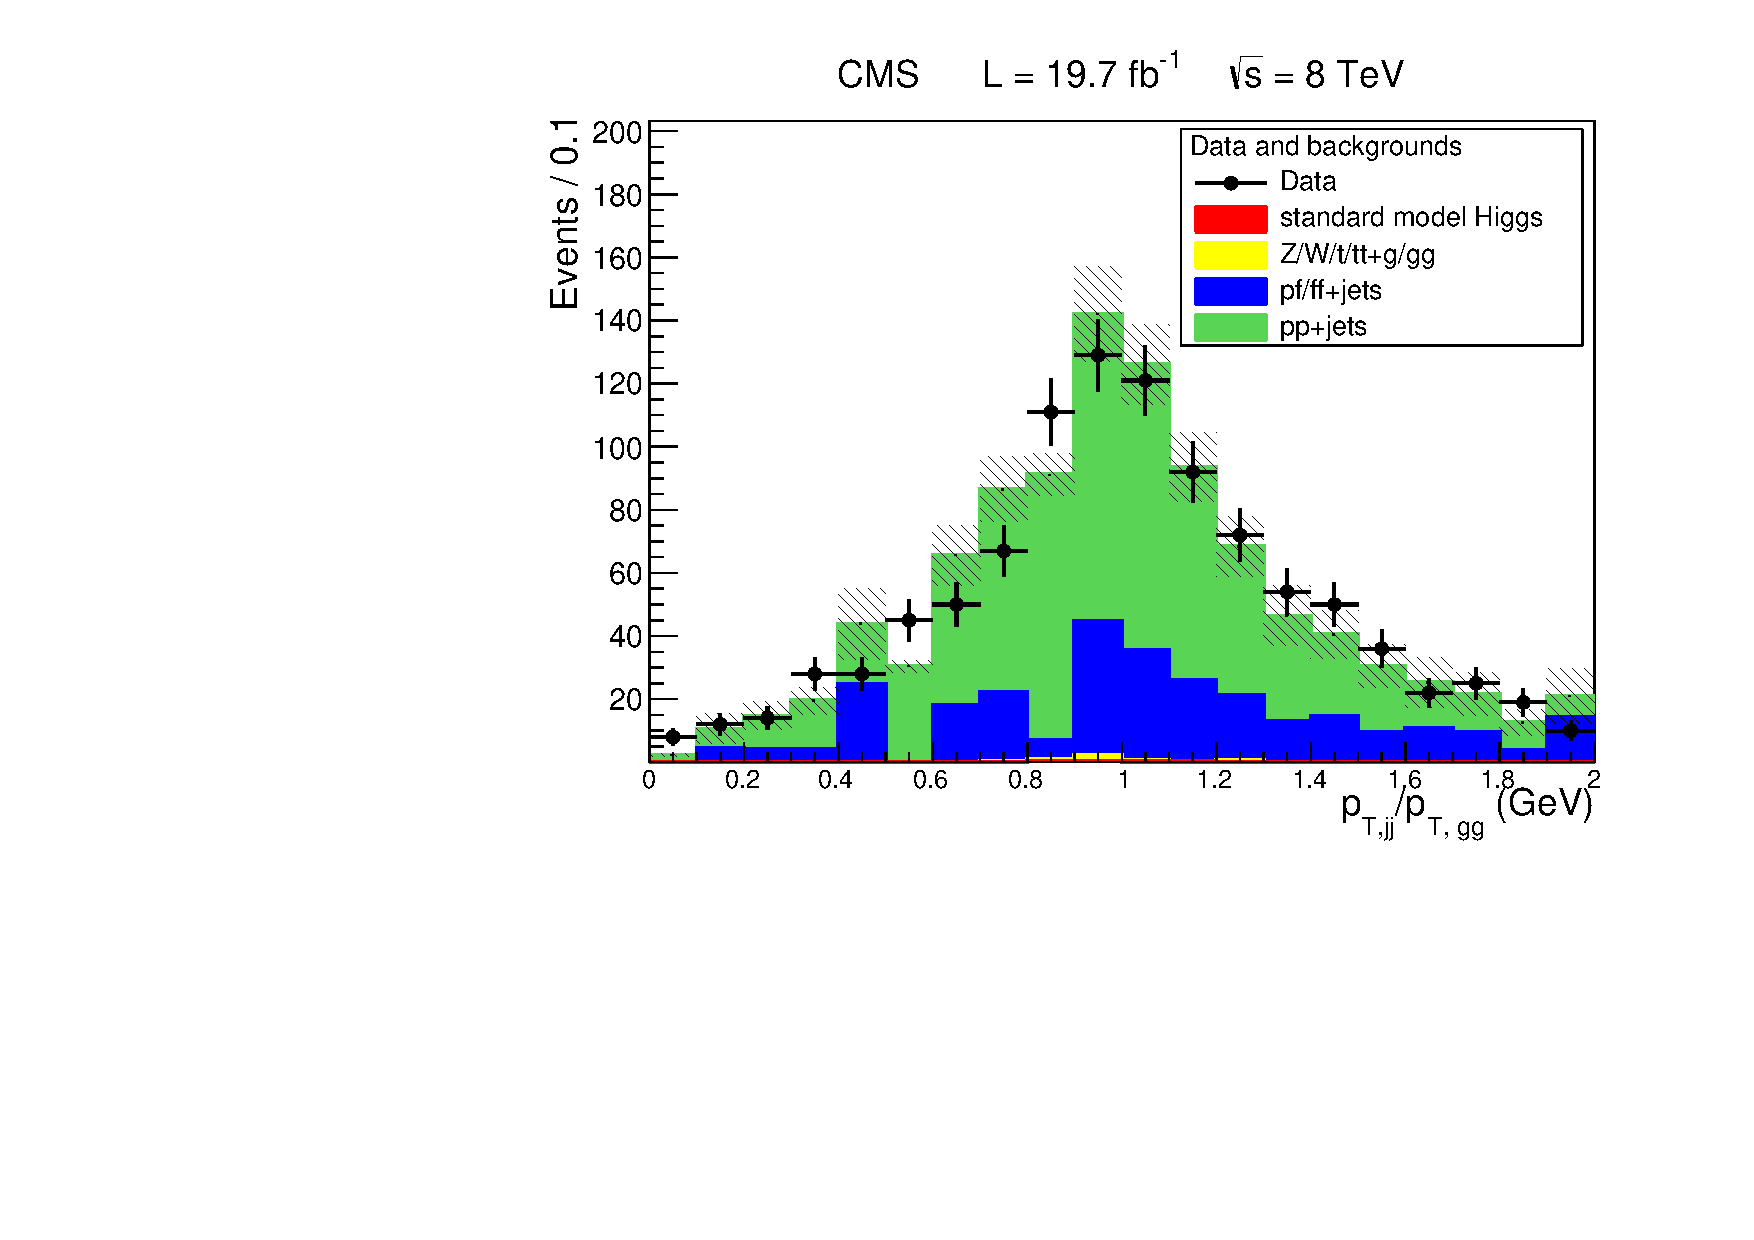
\includegraphics[width=.7\textwidth]{figures/objects/pt_balance_datavsmc_before.pdf}
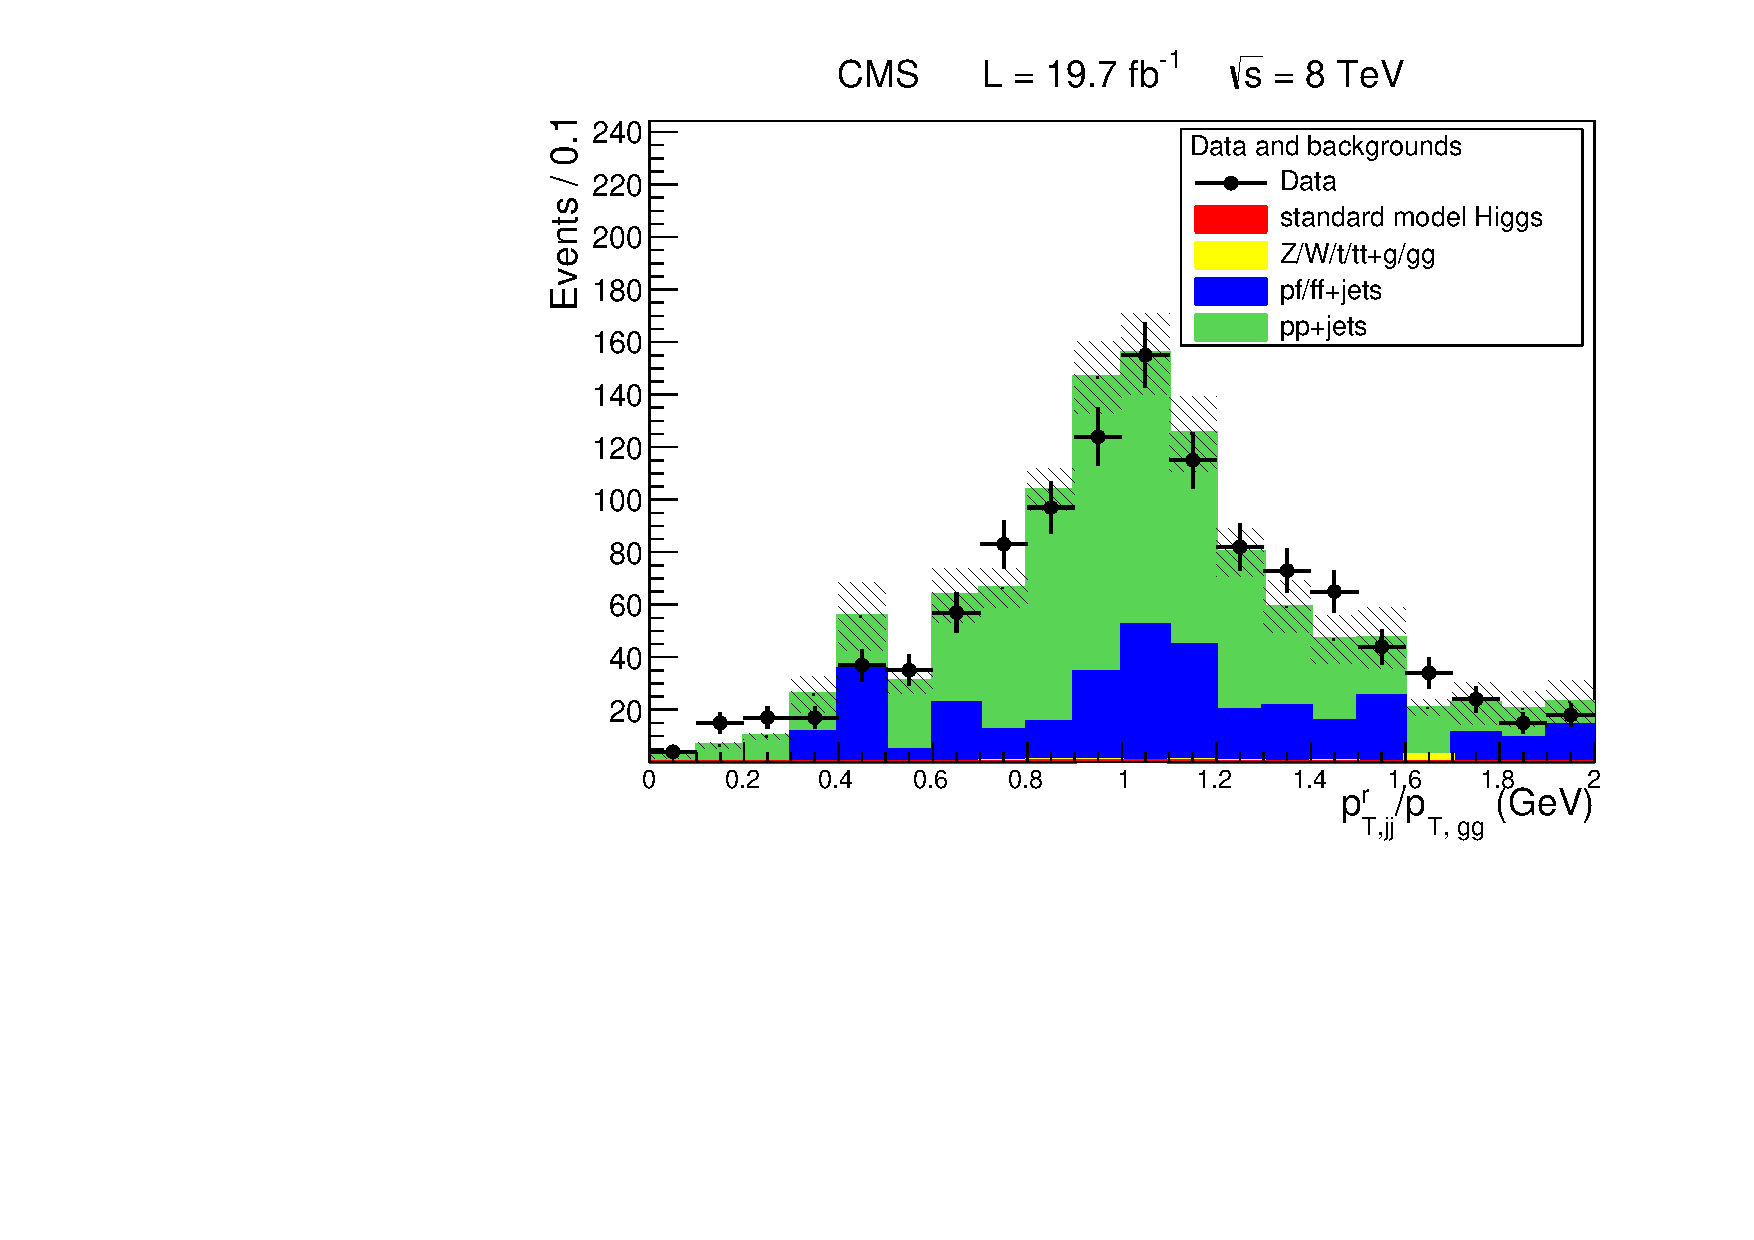
\includegraphics[width=.7\textwidth]{figures/objects/pt_balance_datavsmc_after.pdf}
\end{center}
\caption{Improvement in the $p_{\rm T}$ balance before (top) and after (bottom) the regression is
applied for a comparison between data and the sum of background processes. The events are a combination
of the 1-tag and 2-tag categories with an additional requirement that there be no jets other than
the two from the $\Hbb$ decay.}
\label{fig:regression_validation_datavsmc} 
\end{figure}

%\chapter{Background Processes\label{ch:backgrounds}}

\section{Real processes\label{sec:realbgd}}

\section{Fakes\label{sec:fakebgd}}

\section{Simulation\label{sec:bkgsim}}


\chapter{Event Selection\label{ch:selection}}

This chapter discusses additional event-wide requirements imposed to further
improve the sensitiviy of selecting the signal of interest over the background contributions
beyond that of the preselection requirements covered in Chapter~\ref{ch:objects}.
Event classification is covered in Section~\ref{sec:classification}, in which two classes of
events are defined for extracting signal separately.
Section~\ref{sec:higgsreconstruction} discusses how the photons and jets passing the preselection
requirements are assembled into Higgs candidates. For the resonant search $X\rightarrow HH$,
Section~\ref{sec:Xreconstruction} discusses how the two Higgs come together to construct a resonant
candidate. Finally, the construction of a data control
sample, discussed in Section~\ref{sec:dataCS}, allows for the study of additional event-wide
requirements for improving sensitivity, discussed in Section~\ref{sec:optim}.

\section{Event Classification\label{sec:classification}}

The working point used for signal extraction the medium one (CSVM),
which corresponds to an efficiency of around 60--70\%
and a mistag rate 1--2\%, depending on the jet $p_{\rm T}$.
There is also a tight working point (CSVT) which corresponds to ta mistag rate of 0.1\%.

In order to improve the signal sensitivity, events are classified into three categories
based on the number of CSVM b-tagged jets. Events with two or more b-tags, called high purity,
drive the sensitivity of the search. Events with one b-tag, called medium purity,
bring low contribution but allow for increased signal acceptance. Events without any b-tags,
called low purity, are only used for cross-checks and are rejected from the main analysis.

include table of cuts here

\section{Higgs Reconstruction\label{sec:higgsreconstruction}}

From the lists of photons and jets passing the identification and kinematic requirements, Higgs
candidates 

talk about photon choice, jet choice

The  Higgs  boson  candidate  is  reconstructed  in  the  medium-purity  events  by  pairing  the  b-
tagged jet with the non b-tagged jet giving largest
p
T
of the pair.  For the high-purity events
the pair of b-tagged jets giving the largest
p
T
for the Higgs candidate is used.  This procedure
selects the correct jets in more than 80% of the cases and does not produce any local peaking
structure in the background.
The resulting signal mass shape of the Higgs candidate decaying into two b-quarks is shown on
the Figure 1 (top-right). For the high-purity category, the typical resolution, defined as the half-
width at half-maximum, decreases from 20 GeV at
m
X
=
300 GeV to 15 GeV at
m
X
=
1 TeV. In
the medium-purity category, the resolution is worse, decreasing from 25 GeV at
m
X
=
300 GeV
to 15 GeV at
m
X
=
1 TeV.



\section{Resonance Reconstruction and Kinematic Fit\label{sec:Xreconstruction}}

\section{Data Control Sample\label{sec:dataCS}}

\section{Optimization Studies\label{sec:optim}}
Separate resonant and nonresonant here



\chapter{Systematic Uncertainties\label{ch:uncertainties}}

The expected signal yield is estimated through simulation, corrected
due to limitations to exactly produce what is observed in data.
Corrections imposed in this analysis are related to the photon and jet reconstruction and identification
and related to b-tagging.
The uncertainties associated with these corrections are applied to the reconstructed objects in
the simulation through scaling and smearing the observables of interest.
For the recorded luminosity, the normalization uncertainty is 2.6\%~\cite{CMS-PAS-LUM-13-001}.
The other sources are separated in terms of uncertainties related to photons, jets, and theory,
which are covered in Sections~\ref{sec:photonunc}, \ref{sec:jetunc}, and \ref{sec:theoryunc},
respectively.

\section{Photon Uncertainties\label{sec:photonunc}}

The photon-related uncertainties consist of those pertaining to the photon energy resolution (PER)
and the photon energy scale (PES)~\cite{CMS-PAS-HIG-13-001}. As a function of the
electromagnetic shower shape and $\eta_\gamma$,
an uncertainty between 0.23\% and 0.93\% is imposed on the PER,
and an uncertainty between 0.12\% and 0.88\% on the PES. For hard photons, namely those with
$p_{{\rm T},\gamma} > 100$~GeV, the uncertainty on PES is increased to 1\%.
%These uncertainties are propogated through to the spectra of interest. For the $\Mgg$ spectrum,
%they give  uncertainties on the position and spread of the signal shape. For the
%$\Mggjjk$ spectrum, they give uncertainties on both the position and spread of the signal shape
%and on the normalization.

The photon preselection efficiency contributes a 1\% normalization uncertainty to the $\Mgg$
spectrum. The diphoton trigger efficiency contributes a 1\% normalization
uncertainty to all spectra.
An additional normalization uncertainty of 5\% is imposed in the high-mass resonant search
to account for the differences in the $p_{\rm T}$ spectrum between photons of the signal
and the electrons from $Z\rightarrow e^+ e^-$ used to estimate the PES and PER and their
corresponding uncertainties.

\section{Jet Uncertainties\label{sec:jetunc}}

The jet energy scale (JES) uncertainty is found by varying the jet $p_{\rm T}$ by 1--2\%,
depending on the jet $p_{\rm T}$ and $\eta$~\cite{JINST6}.
The jet energy resolution (JER) uncertainty is found by varying the jet resolution by 10\%.
In the high-mass search, the jets tend to have a higher boost and be closer together,
and effects related to their partial overlap are accounted for with an additional uncertainty of 1\%.
For the b-tagging efficiency uncertainty, the b-tagging scale factors are varied by one standard
deviation in each category~\cite{BTV}. 
The uncertainty for the b-tagging efficiency between the two categories
was found to have negative correlation.

\section{Theory Uncertainties\label{sec:theoryunc}}

No theory uncertainties are imposed for the resonant or nonresonant signal.
For the resonant background, theory uncertainties are imposed on the SM Higgs contribution. These
include contributions from missing order effects and the dependency on proton parton density
functions~\cite{Dittmaier:2011ti,Heinemeyer:2013tqa}.
A systematic uncertainty is imposed on the Higgs mass for both for the resonant or nonresonant signal
and for the resonant background.
This uncertainty of 0.45 GeV is taken from the Higgs mass measurement performed at CMS in the
$H\rightarrow ZZ \rightarrow 4\ell$ channel~\cite{Chatrchyan:2013mxa}.

\section{Summary and Impact on Analysis\label{sec:uncimpact}}

The impact of the quoted systematic uncertainties on the result is summarized in
Table~\ref{table:systematics}.
The analysis is statistics limited, and the systematic uncertainties worsen the expected limits
by at most 1.7\% (3.8\%) in the resonant (nonresonant) search.

\begin{table}[ht]
  \centering
  \renewcommand{\arraystretch}{1.4}
  \caption{Systematic uncertainties organized by search strategy.}
  \begin{tabular}{|c|c|}
\hline
\multicolumn{2}{|c|}{Common normalization uncertainties} \\
\hline
Luminosity & 2.6\%\\
Diphoton trigger acceptance & 1.0\% \\
\hline
\hline
\multicolumn{2}{|c|}{fit $M_{\gamma\gamma}$ - Background dominated} \\
\hline
\hline
\multicolumn{2}{|c|}{Normalization uncertainties} \\
\hline
Photons selection acceptance & 1.0\% \\ 
"b-tag" eff. uncertainty 2 btag cat & 4.6\% \\  
"b-tag" eff. uncertainty 1 btag cat & -1.2\% \\  
$M_{jj}$ and $p_{T, j}$ cut acceptance ( JES \& JER) & 1.5\%\\
$M_{\gamma\gamma\rm jj}$ cut acceptance (PES $\oplus$ JES \& PER  $\oplus$ JER) & 2\%\\
\hline
\multicolumn{2}{|c|}{Shape uncertainties} \\
\hline
Parametric scale shift (PES$\oplus$M(H) uncertainty)      & $\frac{\Delta M_{\gamma \gamma}}{M_{\gamma \gamma}} = 0.45 \oplus 0.35$\%\\
Parametric resolution shift (RES) & $\frac{\Delta \sigma}{M_{\gamma \gamma}} = 0.25$\% \\
                                  & $\frac{\Delta \sigma}{\sigma_{\gamma \gamma}} = 22$\% \\
\hline
\hline
\multicolumn{2}{|c|}{fit $M_{\gamma\gamma\rm jj}$ - Background dominated} \\
\hline
\hline
\multicolumn{2}{|c|}{Normalization uncertainties} \\
\hline
Photons selection acceptance & 1.0\% \\ 
"b-tag" eff. uncertainty 2 btag cat & 5.3\% \\  
"b-tag" eff. uncertainty 1 btag cat & -1.8\% \\  
$M_{jj}$ and $p_{T, j}$ cut acceptance ( JES \& JER) & 1.5\%\\
$M_{\gamma\gamma}$ cut acceptance (PES \& PER ) & 0.5\% \\
Extra High pt norm. uncertainty & 5.0\% \\
\hline
\multicolumn{2}{|c|}{Shape uncertainties} \\
\hline
Parametric abs. shift (PES $\oplus$ JES ) & $\frac{\Delta M_{\gamma \gamma {\rm jj} }}{M_{\gamma \gamma {\rm jj} }} = 0.45 \oplus (0.8 \oplus 1.0) = 1.4$\% \\
Parametric shift (PER $\oplus$ JER ) & $\frac{\Delta \sigma}{\sigma_{\gamma \gamma {\rm jj} }} = 10$\% \\
\hline
\end{tabular}

  \label{table:systematics}
\end{table}

\chapter{Results\label{ch:results}}

After applying the preselection, event classification, and mass windows, the signal efficiency
and event yields are examined, as discussed in Section~\ref{sec:yields}. Then the signal yield
in data is evaluated through the calculation of the confidence level (CL)
for discovery or exclusion of double Higgs production. This is evaluated from a simultaneous fit
to the $\Mgg$, $\Mggjjk$, and $\Mgg \times \Mjj$ spectra for the low-mass resonant, high-mass resonant,
and nonresonant searches, respectively.
To compute the upper limits on the production cross section, the modified frequentist approach
$\text{CL}_s$ is used with an asymptotic approximation, taking the profile likelihood as a test
statistic~\cite{CLS1,CLS2}. This calculation is discussed in Section~\ref{sec:resresults} for the
resonant search and in Section~\ref{sec:nonresresults} for the SM nonresonant search.

\section{Signal Efficiencies and Yields\label{sec:yields}}

The signal efficiency as a function of $m_X$ for the resonant search is summarized in
Figure~\ref{fig:eff_res}. The signal efficiency increases from 260 GeV to 900 GeV
due to improved photon and jet reconstruction. The signal efficiency
peaks at and drops after 900 GeV due to the merging of the two jets from the decay $\Hbb$ into
a single jet. For future consideration in extending the search above 1.1 TeV,
jet substructure techniques would be necessary to resolve the merging of the two
jets~\cite{Ellis:2009su}.
Both categories contribute approximately equally to the overall efficiency.

\begin{figure}[ht!]
 \begin{center}
    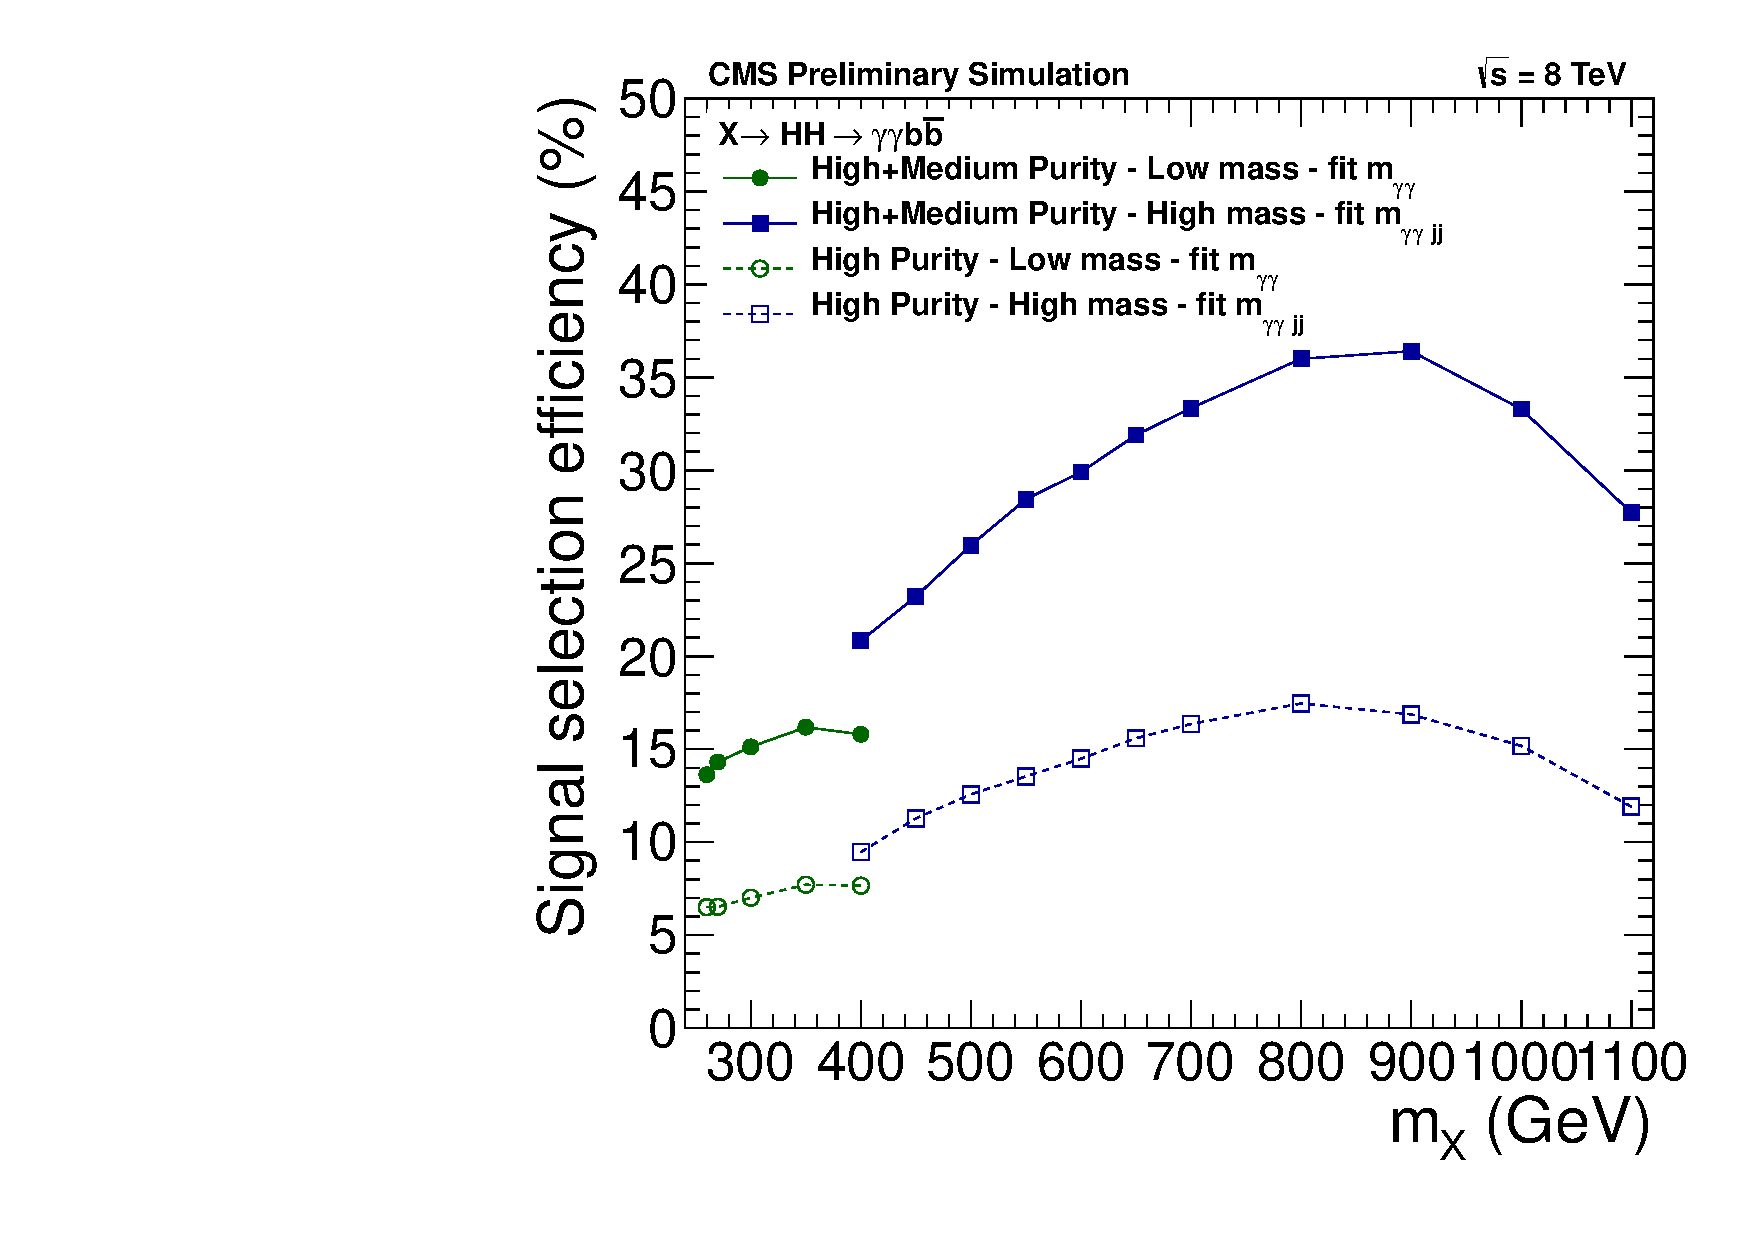
\includegraphics[width=0.55\textwidth]{figures/results/eff_all.pdf}
      \end{center}
\caption{Signal efficiency for the resonant search for the final selection.}
\label{fig:eff_res}
\end{figure}

The yields for the low-mass resonant search at $m_X = 300$~GeV are summarized in
Table~\ref{table:yield_lowmass_res}. Note that there is a normalization disagreement in the
$\gamma\gamma j$ and $\gamma j$ contributions as the simulation has limitations in modeling
QCD with one or two hard photons. As a result, the backgrounds are not added; the purpose is to
highlight relative contributions to the nonresonant background.
The yields for the high-mass resonant search are summarized in
Table~\ref{table:yield_highmass_res}. For this search, the requirements are independent of
the mass hypothesis, so several signal hypotheses can be shown together.

\begin{table}[ht!]
  \centering
  \renewcommand{\arraystretch}{1.4}
  \caption{Event yields for the low-mass resonant search at 300 GeV. Expectations are given for
the signal, resonant background, and nonresonant background. Counts are given for data. Note that
there is a normalization disagreement coming from the shortcomings of simulating QCD with one
or two hard photons.}
  \begin{tabular}{|c|c|c|}
\hline
Sample & High purity & Medium purity\\
\hline
Radion (300$~$GeV, $\Lambda_R$=1TeV)  & 18.73 & 21.66     \\
\hline
ggF $\Hgg$                &  0.02  &  0.19 \\
VBF $\Hgg$                &  0.00  &  0.04 \\
$WH(\gamma\gamma)$        &  0.00  &  0.05 \\
$ZH(\gamma\gamma)$        &  0.00  &  0.03 \\
$t\bar{t}H(\gamma\gamma)$ &  0.10  &  0.15 \\
\hline
$\gamma\gamma j$                      & 8.9  &  188  \\
$\gamma j$                            & 0.00 &  9.2  \\ 
QCD                                   & 0.00 &  0.00 \\ 
$Z/\gamma^*\rightarrow\ell^+\ell^- + Z(\ell^+\ell^-)\gamma + W(\ell\nu)\gamma\gamma$ & 0.00 &  0.21 \\
$t\bar{t}\gamma\gamma + t\gamma\gamma + t\bar{t}\gamma j$ & 0.44 &  1.2  \\
\hline
Data                                  & 21 & 230 \\
\hline
\end{tabular}

  \label{table:yield_lowmass_res}
\end{table}

\begin{table}[ht!]
  \centering
  \renewcommand{\arraystretch}{1.4}
  \caption{Event yields for the high-mass resonant search. Expectations are given for
the signal, resonant background, and nonresonant background. Counts are given for data. Note that
there is a normalization disagreement coming from the shortcomings of simulating QCD with one
or two hard photons.}
  \begin{tabular}{|c|c|c|}
\hline
Sample & High purity & Medium purity\\
\hline
Radion (500$~$GeV, $\Lambda_R$=1TeV)        &  6.08  & 6.47     \\
Radion (700$~$GeV, $\Lambda_R$=1TeV)        &  2.92  & 3.03     \\
Radion (1000$~$GeV, $\Lambda_R$=1TeV)       &  0.94  & 1.12     \\
\hline
ggF $\Hgg$                &  0.07  &  0.6  \\
VBF $\Hgg$                &  0.01  &  0.12 \\
$WH(\gamma\gamma)$        &  0.00  &  0.10 \\
$ZH(\gamma\gamma)$        &  0.03  &  0.07 \\
$t\bar{t}H(\gamma\gamma)$ &  0.24  &  0.50 \\
\hline
$\gamma\gamma j$                      & 3.0  &  70   \\
$\gamma j$                            & 0.00 &  3.0  \\
QCD                                   & 0.00 &  0.00 \\
& 8.9  &  188  \\
& 0.00 &  9.2  \\ 
& 0.00 &  0.00 \\ 
$Z/\gamma^*\rightarrow\ell^+\ell^- + Z(\ell^+\ell^-)\gamma + W(\ell\nu)\gamma\gamma$ & 0.00 &  0.08 \\
$t\bar{t}\gamma\gamma + t\gamma\gamma + t\bar{t}\gamma j$ & 0.15 &  0.55 \\
\hline
Data                                  & 8 & 79 \\
\hline
\end{tabular}

  \label{table:yield_highmass_res}
\end{table}

The yields for the nonresonant search are summarized in Table~\ref{table:yield_nonres}.
They are greater in the nonresonant search because the $\Mggjjk$ spectrum is less
discriminating than in the low-mass resonant search and because the $\Mjj$ spectrum is
modeled on the range $\Mjj \in [60,180]$~GeV rather than selected on a narrower window.

\begin{table}[ht!]
  \centering
  \renewcommand{\arraystretch}{1.4}
  \caption{Event yields for the nonresonant search. Expectations are given for
the SM nonresonant signal, resonant background, and nonresonant background.
Counts are given for data. Note that
there is a normalization disagreement coming from the shortcomings of simulating QCD with one
or two hard photons.}
  \begin{tabular}{|c|c|c|c|c|}
\hline
 & \multicolumn{2}{c|}{High Purity} & \multicolumn{2}{c|}{Medium Purity} \\
Sample & high $\Mggjjk$ & low $\Mggjjk$ & high $\Mggjjk$ & low $\Mggjjk$ \\
\hline
SM nonresonant $HH$ & 2.03 & 0.28 & 1.99 & 0.20\\
%SM: $\kapl = 1$, $\kapt = 1$, $\ctwo = 0$ & 2.03 & 0.28 & 1.99 & 0.20\\
%$\kapl = 20$, $\kapt = 1$, $\ctwo = 0$ & 78.7 & 102 & 86.5 & 96.5\\
%$\kapl = 1$, $\kapt = 1$, $\ctwo = -2$  & 103 & 16.2 & 101 & 16.5\\
%lam=1  yt=1 c2=0  xsec = 9.96
%lam=20 yt=1 c2=0  xsec = 1046
%lam=1  yt=1 c2=-2 xsec  = 511
\hline
ggF $\Hgg$                &  0.05 & 0.04 & 0.29 & 0.32\\
VBF $\Hgg$                &  0.01 & 0.01 & 0.05 & 0.05\\
$WH(\gamma\gamma)$        &  0.00 & 0.00 & 0.12 & 0.09\\     
$ZH(\gamma\gamma)$        &  0.04 & 0.02 & 0.07 & 0.05\\
$t\bar{t}H(\gamma\gamma)$ &  0.16 & 0.17 & 0.30 & 0.17\\
$b\bar{b}H(\gamma\gamma)$ &  0.00 & 0.01 & 0.01 & 0.04\\  
\hline
$\gamma\gamma j$     &  13 & 21  & 151 & 268 \\
$\gamma j$           & 0.00& 4.3 & 28  & 53  \\
QCD                  & 0.00& 0.00& 0.00& 0.00\\
$Z/\gamma^*\rightarrow\ell^+\ell^- + Z(\ell^+\ell^-)\gamma + W(\ell\nu)\gamma\gamma$
   & 0.00 & 0.01 & 2.3 & 0.18 \\
$t\bar{t}\gamma\gamma + t\gamma\gamma + t\bar{t}\gamma j$ &  1.3 & 2.2 & 3.3 & 3.4 \\
\hline
Data                                  & 41 & 136 & 37 & 319 \\
\hline
\end{tabular}

  \label{table:yield_nonres}
\end{table}

\section{Resonant Results\label{sec:resresults}}

\subsection{Low-mass Resonant Results}

For the low-mass resonant search, the signal yield is extracted by fitting the $\Mgg$ spectrum.
The signal model is built for each mass hypothesis by fitting the $\Mgg$ spectrum
in the simulation sample
separately for the two categories. The functional form used is the sum of a Crystal Ball and
Gaussian with each mean constrained to be the same,
where the former models the core of the distribution and the latter models the
tails. The position of the peak and the spread are independent of the resonant mass and the
category. Figure~\ref{fig:sigfit_300} shows an example of the signal fit for a mass hypothesis of
300 GeV.

\begin{figure}[ht!]
 \begin{center}
   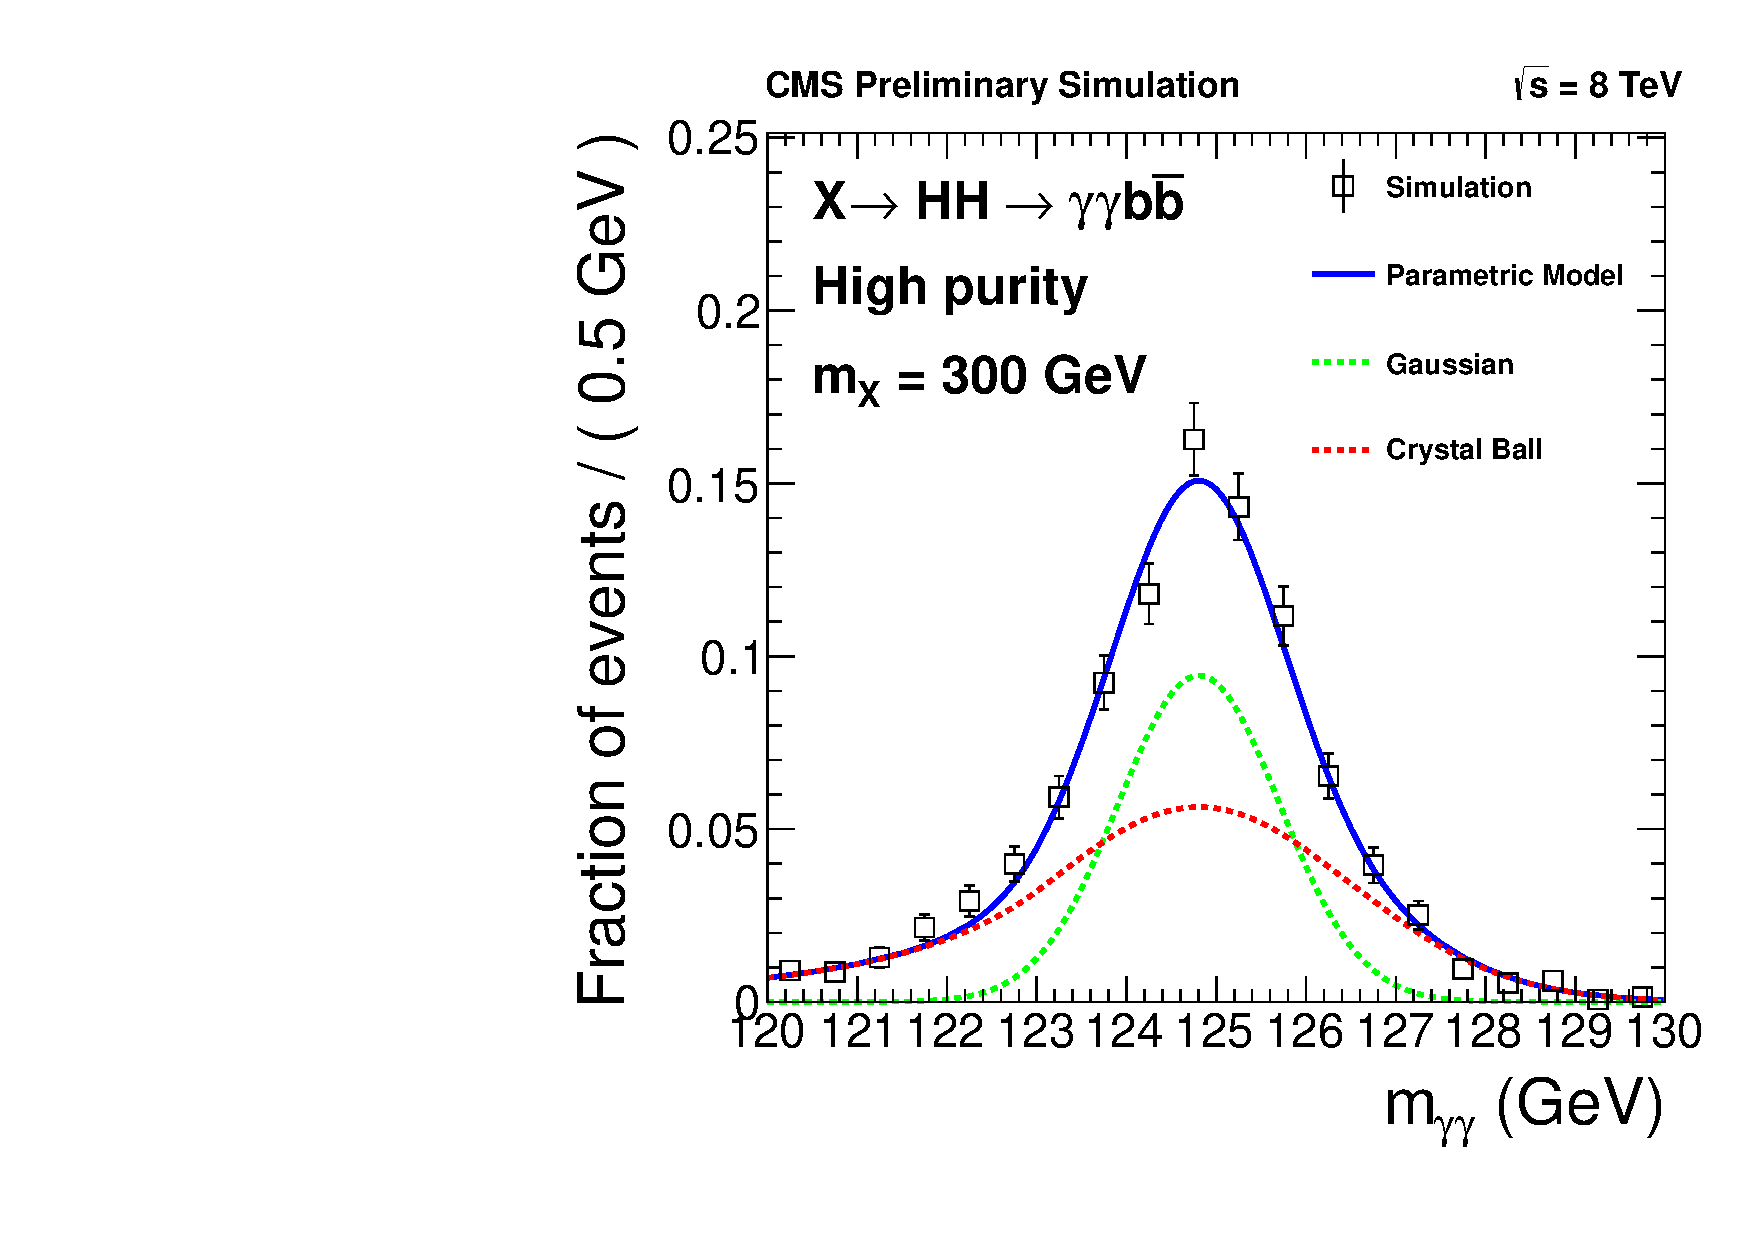
\includegraphics[width=0.45\textwidth]{figures/results/sigmodel_cat0_300.pdf}
   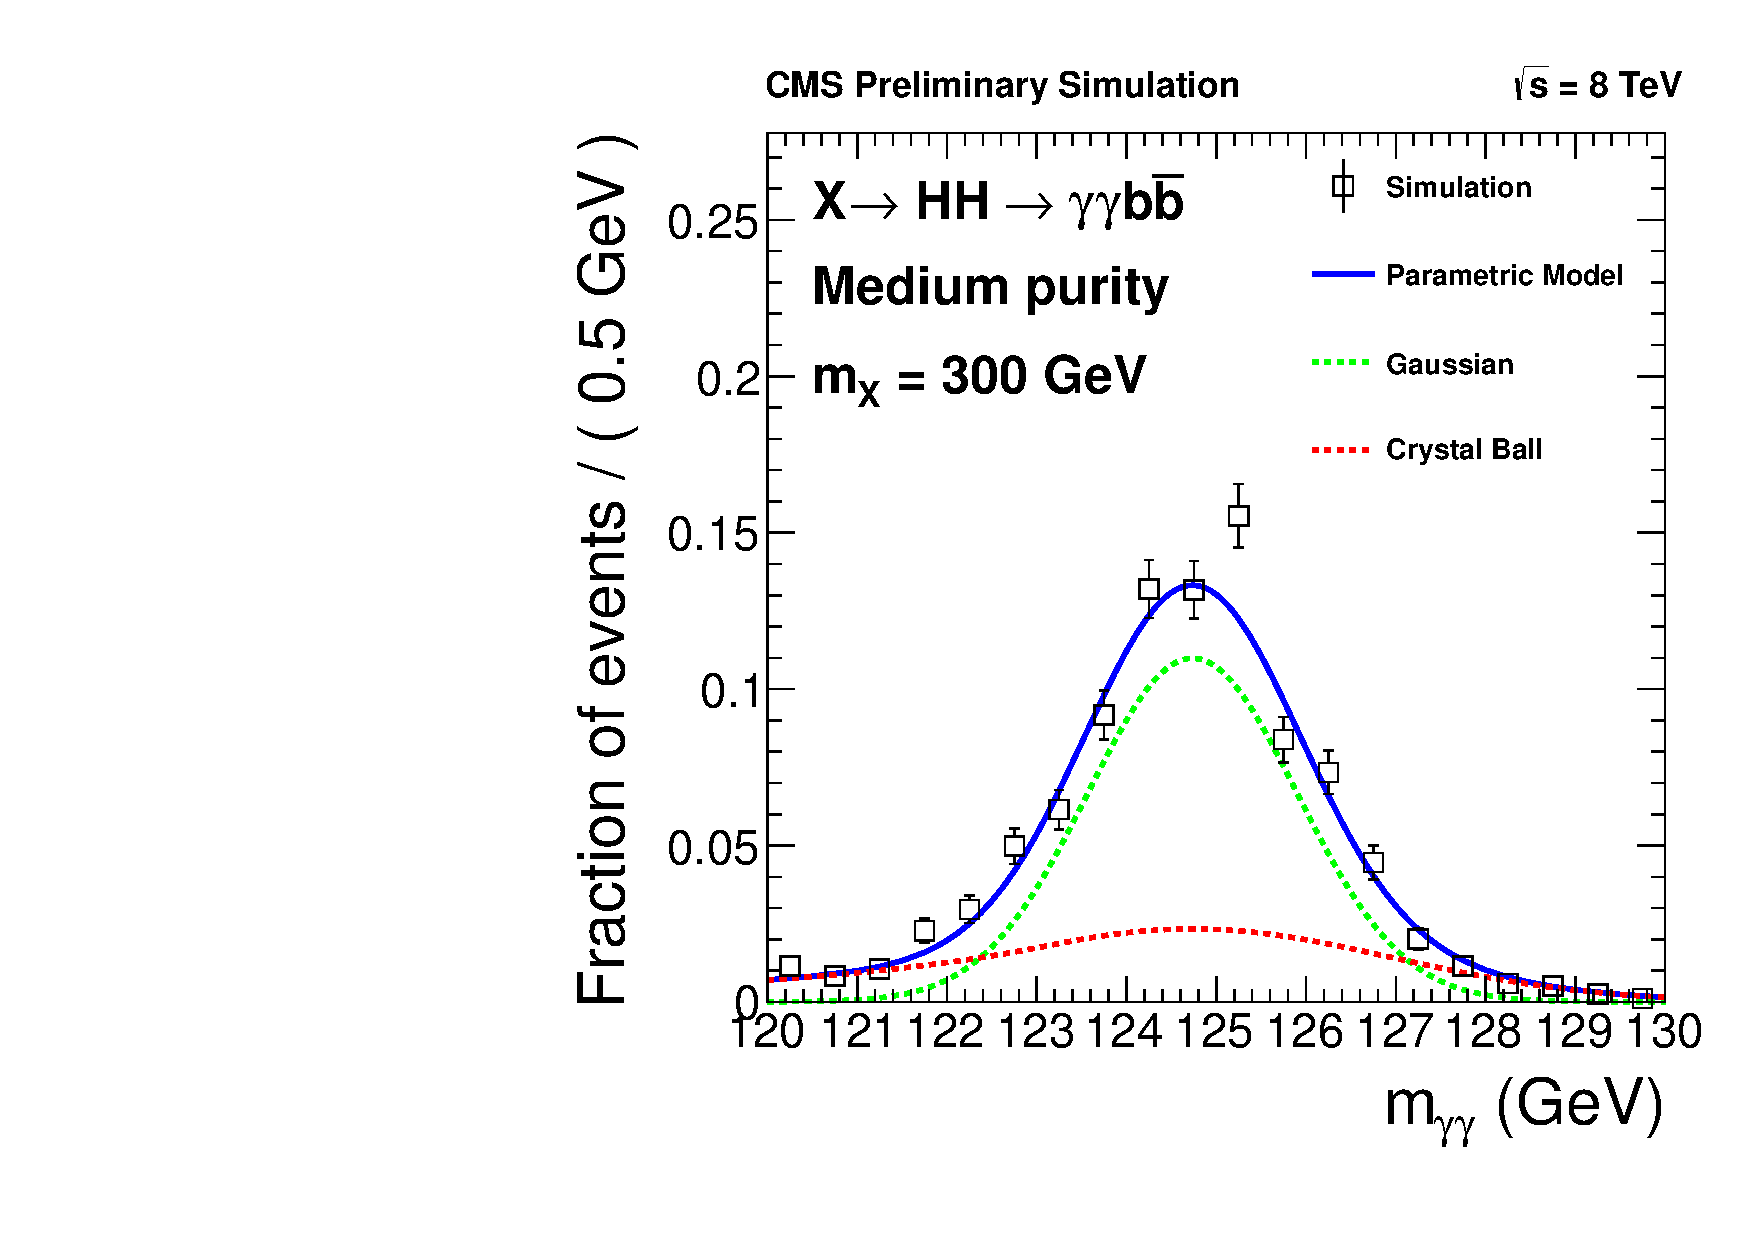
\includegraphics[width=0.45\textwidth]{figures/results/sigmodel_cat1_300.pdf}
 \end{center}
\caption{Simulated signal shape in the $\Mgg$ spectrum for the high-purity (left) and medium-purity
(right) categories for the Radion with mass 300 GeV. The open squares and corresponding
statistical uncertainties represent the simulation.
The blue line represents the signal model fitted to the simulation, while the green dashed line
and the red dashed line represent the two components of the signal model.}
\label{fig:sigfit_300}
\end{figure}

The background estimation is performed by fitting the same distribution in each category on the interval
$[100, 180]$~GeV. This procedure is completely data-driven, and as such it is important
to verify that the choice of the function does not bias in a non-negligible way the
estimate of the signal
strength obtained from the fit to data with the sum of signal and background components.
The bias is estimated by considering a set of truth models which approximately describe the background.
For each truth model a large set of pseudo-data is generated and fitted by the sum of a candidate
background model and the signal model. The bias is defined as the ratio of the extracted signal strength
$\mu$ divided by the associated statistical uncertainty $\sigma_\mu$ and
is considered negligible if
\begin{equation}
\left|\text{median}\left(\frac{\mu}{\sigma_\mu}\right)\right| < 14\% \,.
\end{equation}
For both categories, more than one unbiased background candidate function is identified.
For the limit extraction,
a power law is chosen for both categories. Figures~\ref{fig:datafit_260} and \ref{fig:datafit_300}
shows the background fits to the data for four mass hypotheses.

\begin{figure}[ht!]
 \begin{center}
   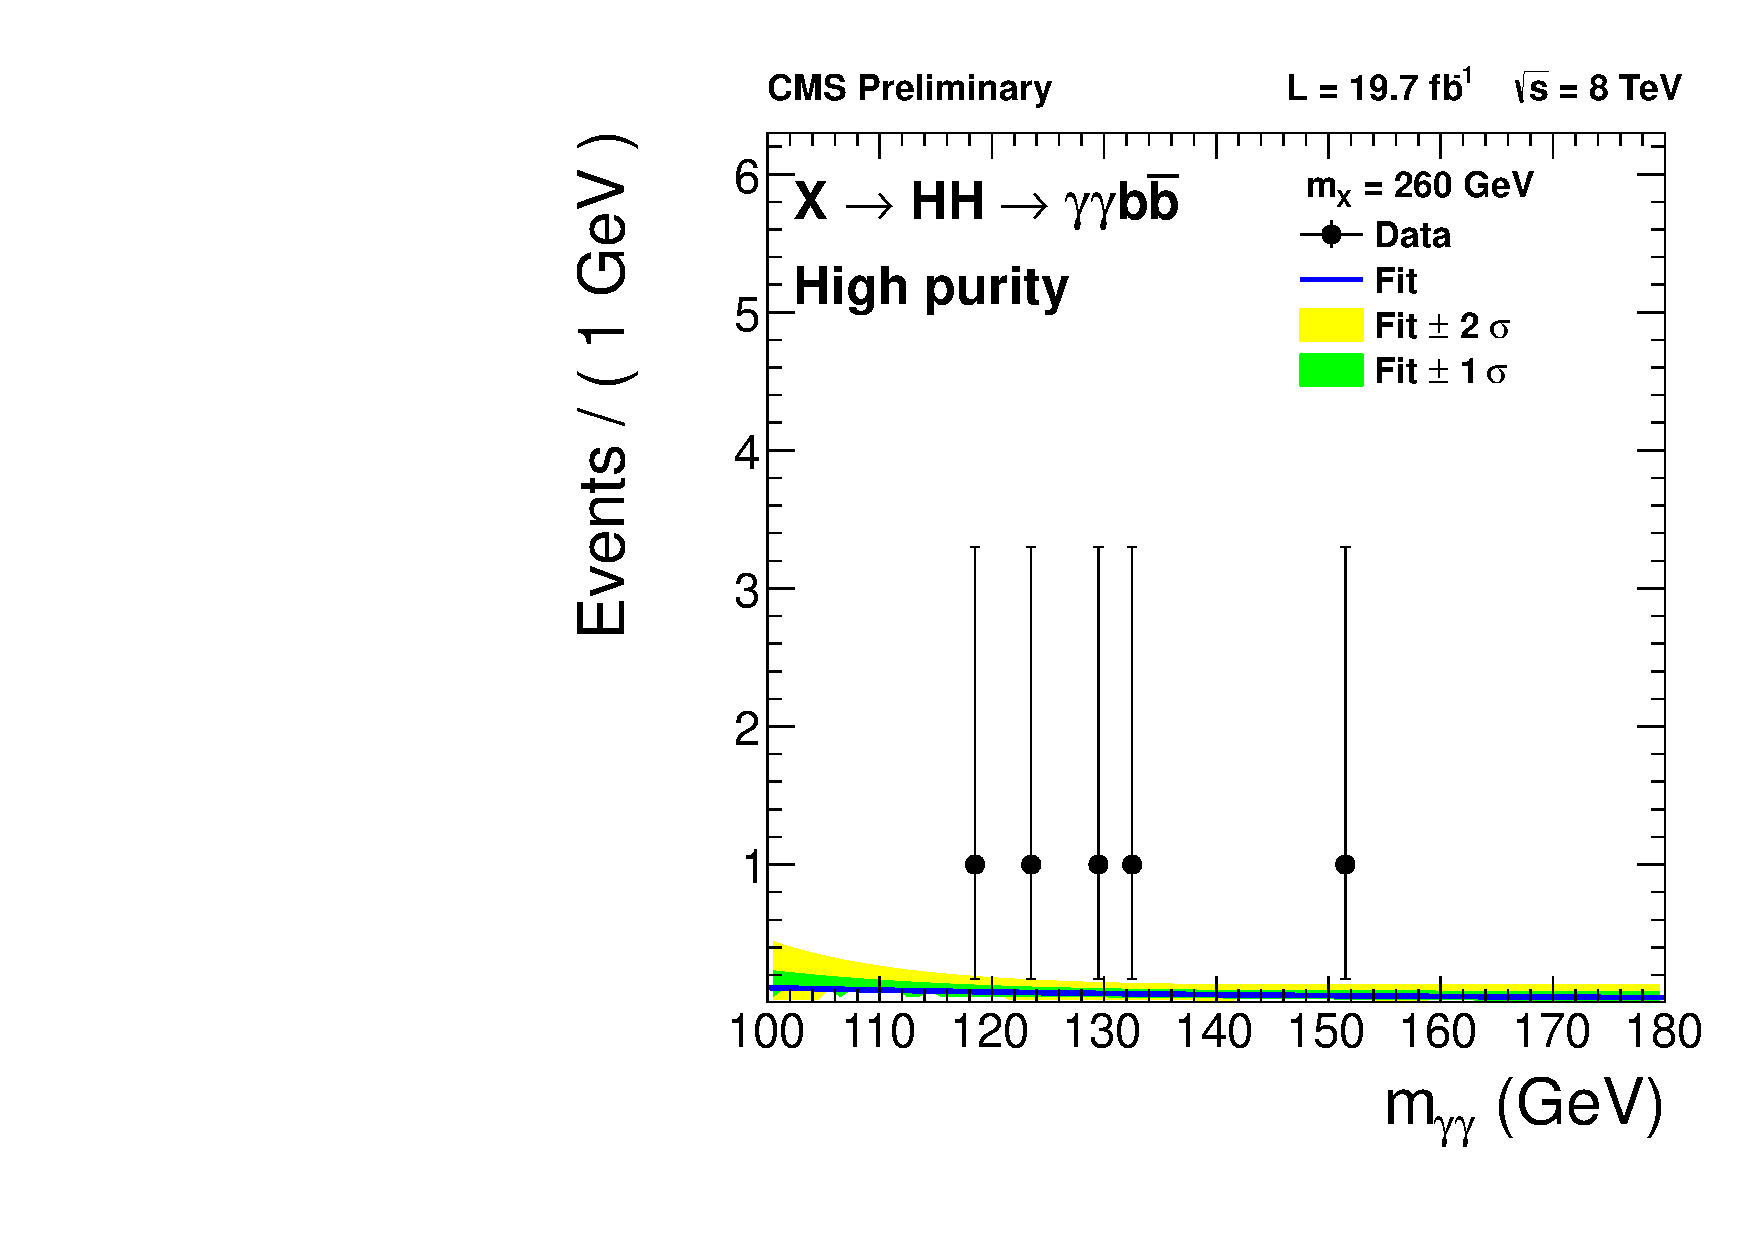
\includegraphics[width=0.45\textwidth]{figures/results/databkgoversig_cat0_260GeV.pdf}
   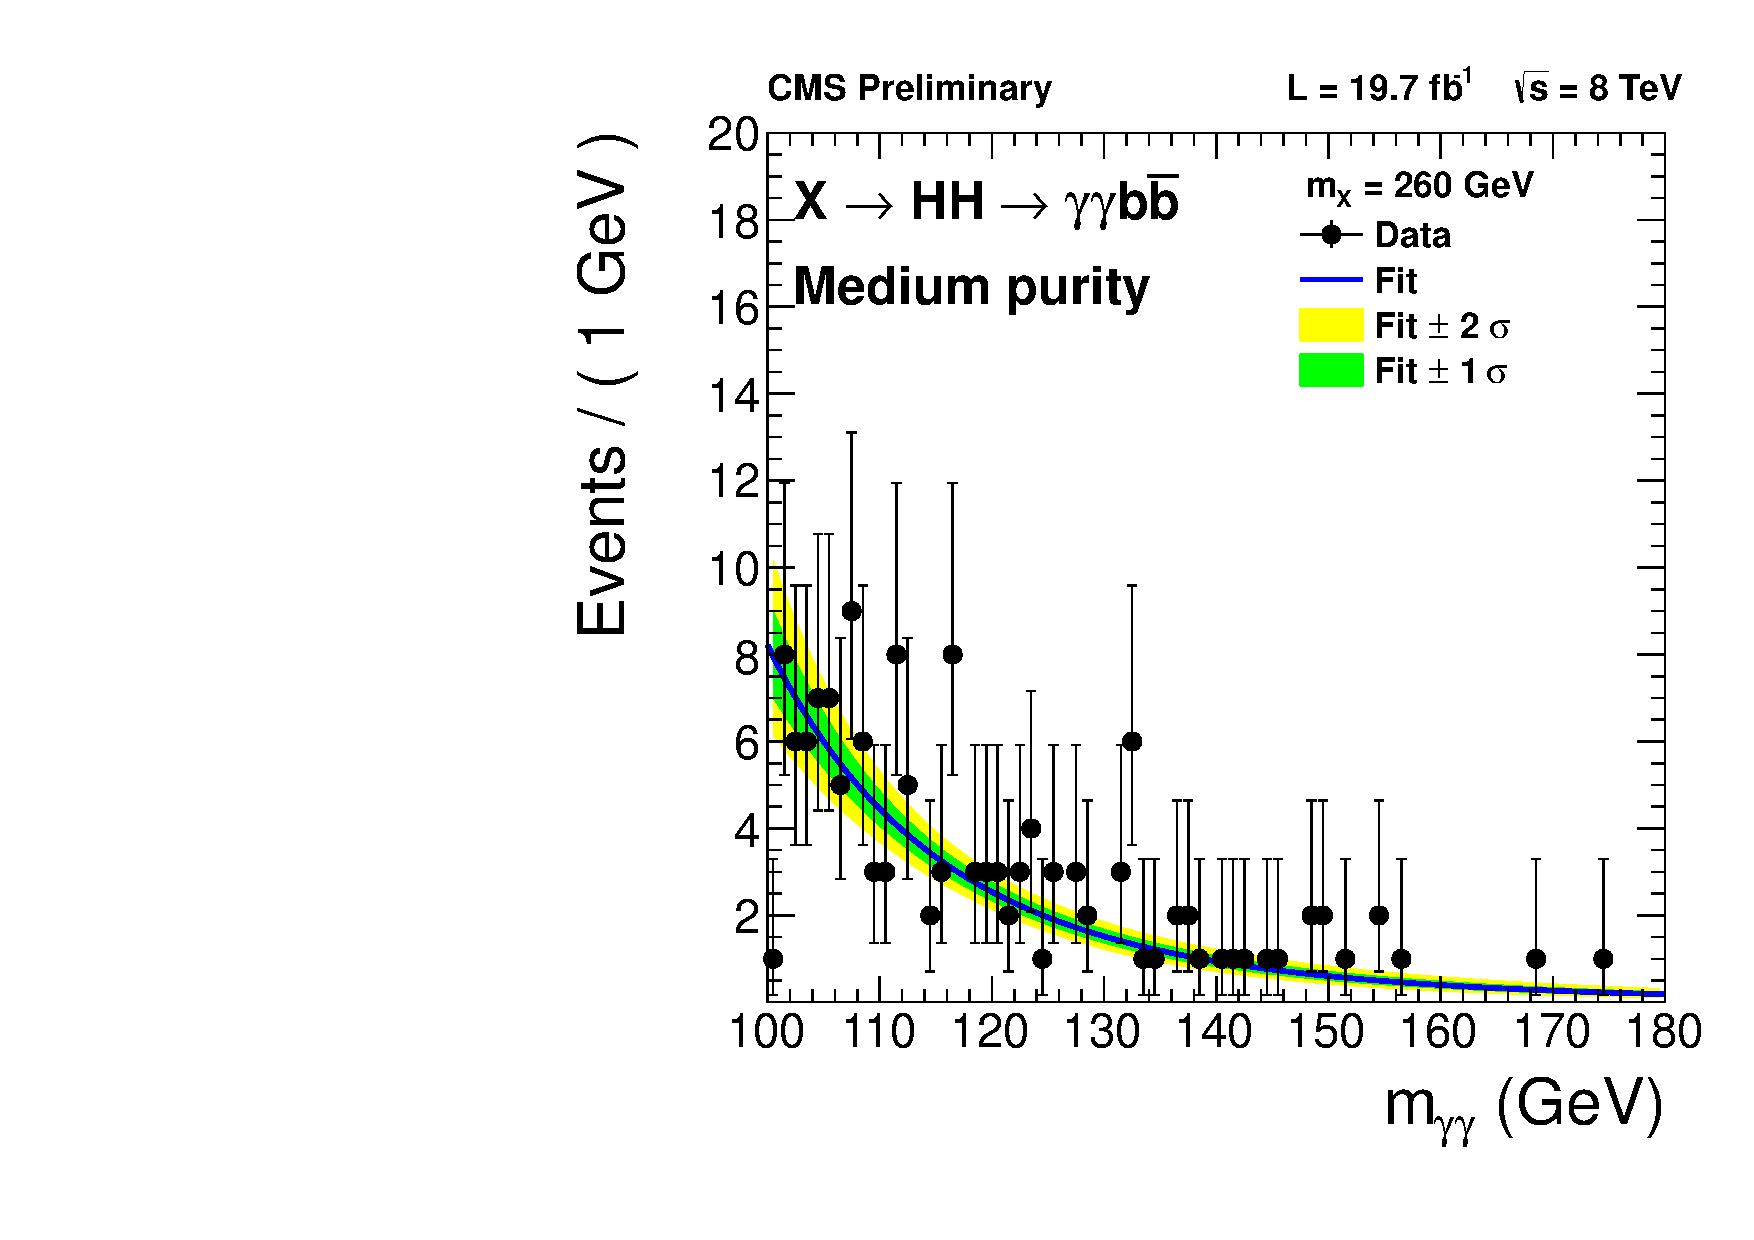
\includegraphics[width=0.45\textwidth]{figures/results/databkgoversig_cat1_260GeV.pdf}
   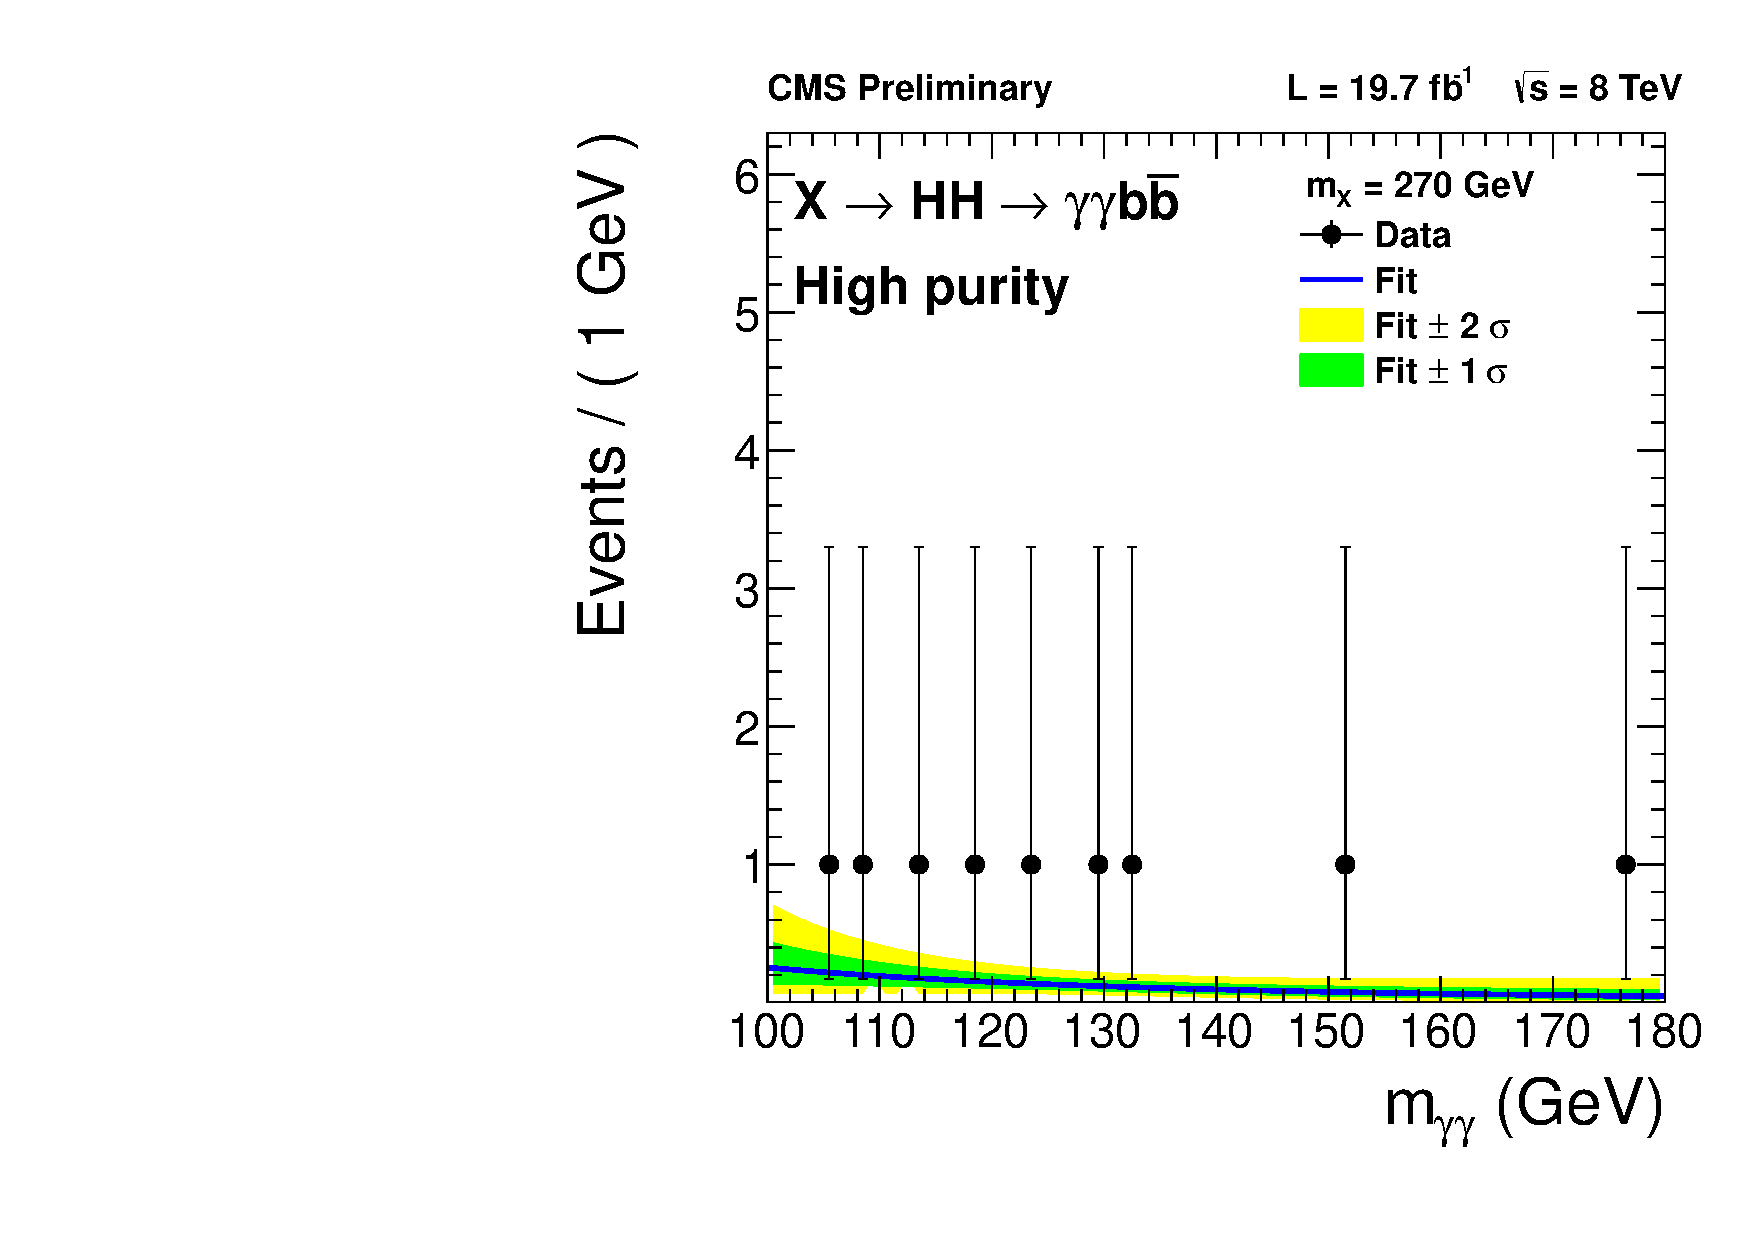
\includegraphics[width=0.45\textwidth]{figures/results/databkgoversig_cat0_270GeV.pdf}
   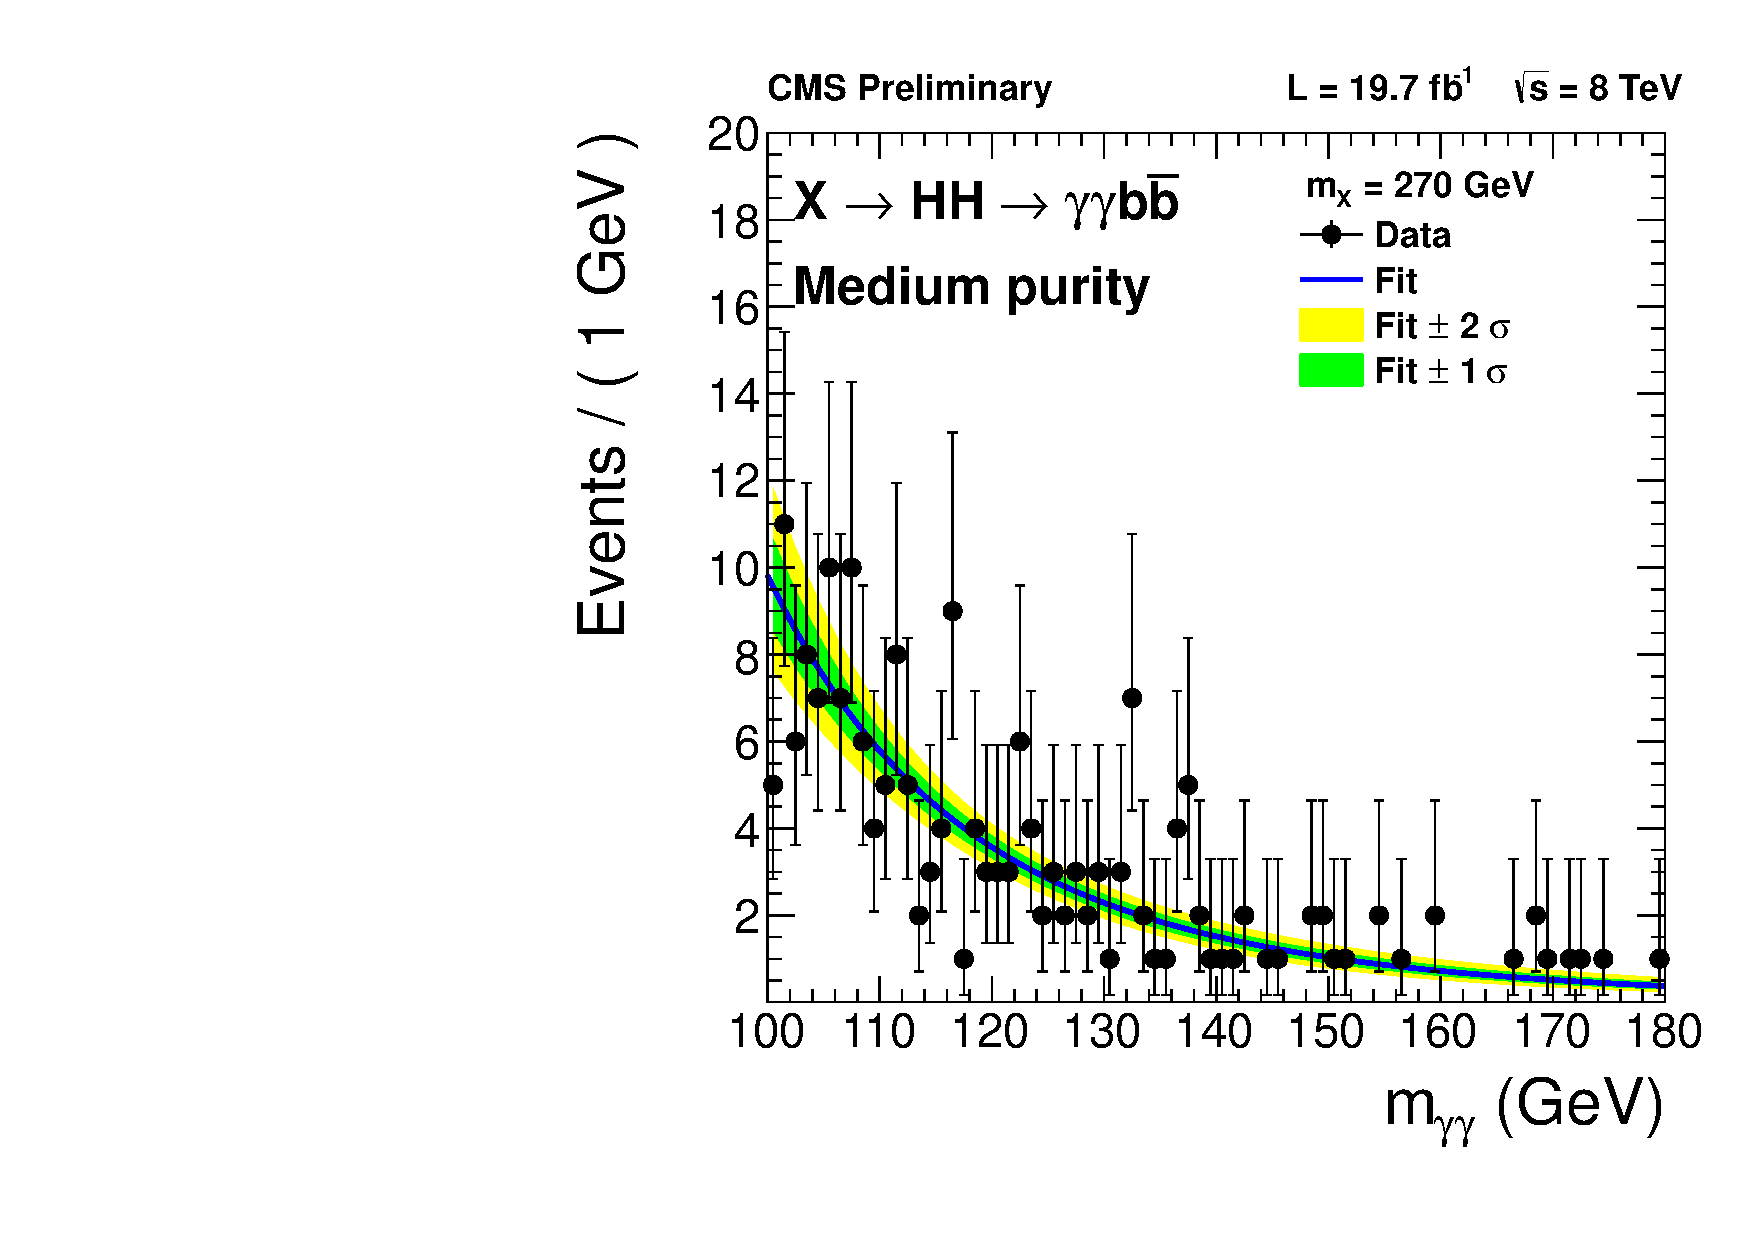
\includegraphics[width=0.45\textwidth]{figures/results/databkgoversig_cat1_270GeV.pdf}
 \end{center}
\caption{Events in the $\Mgg$ spectrum in the high-purity (left column) and medium-purity
(right column) categories for the resonance mass hypotheses 260 GeV (top row) and 270 GeV (bottom row).
The nonresonant component of the background fit is shown in blue
with its corresponding 1$\sigma$ and 2$\sigma$ confidence intervals.}
\label{fig:datafit_260}
\end{figure}

\begin{figure}[ht!]
 \begin{center}
   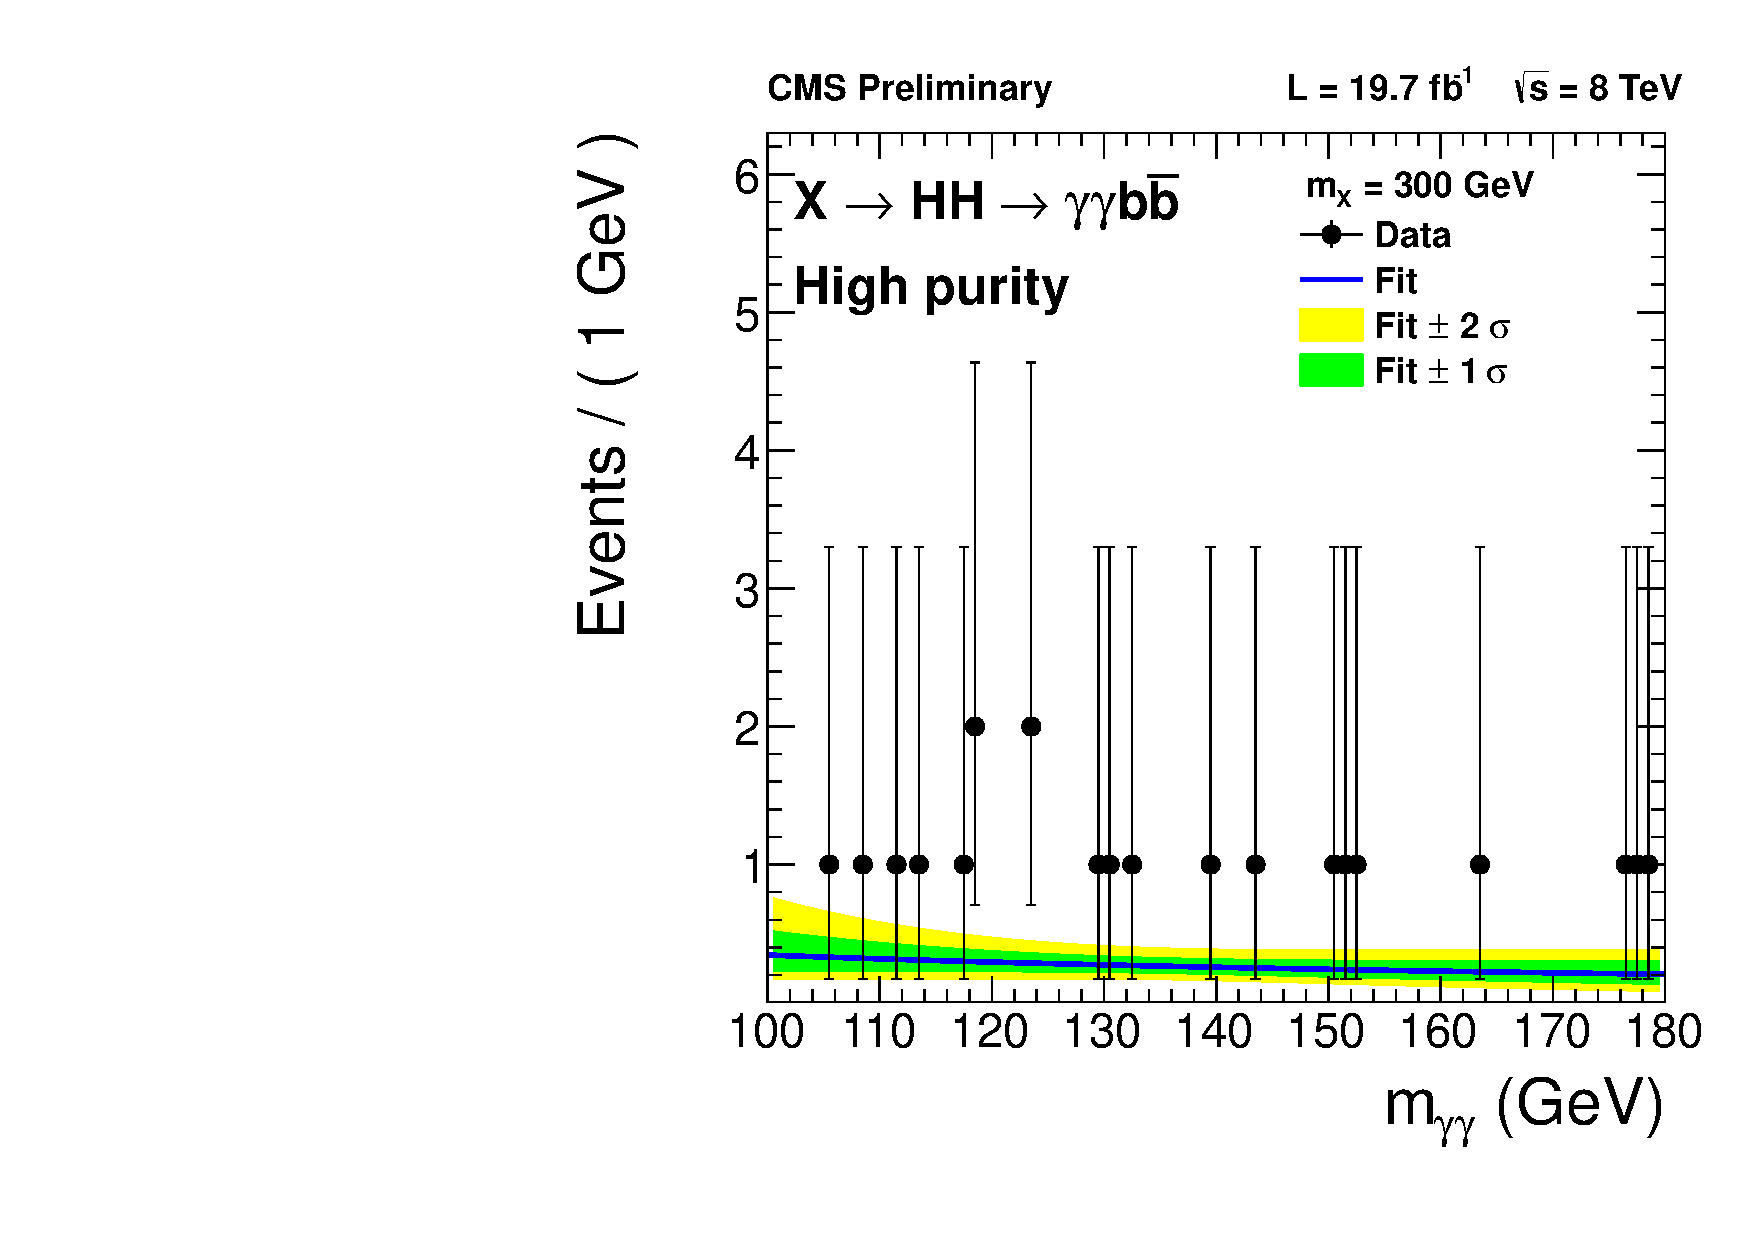
\includegraphics[width=0.45\textwidth]{figures/results/databkgoversig_cat0_300GeV.pdf}
   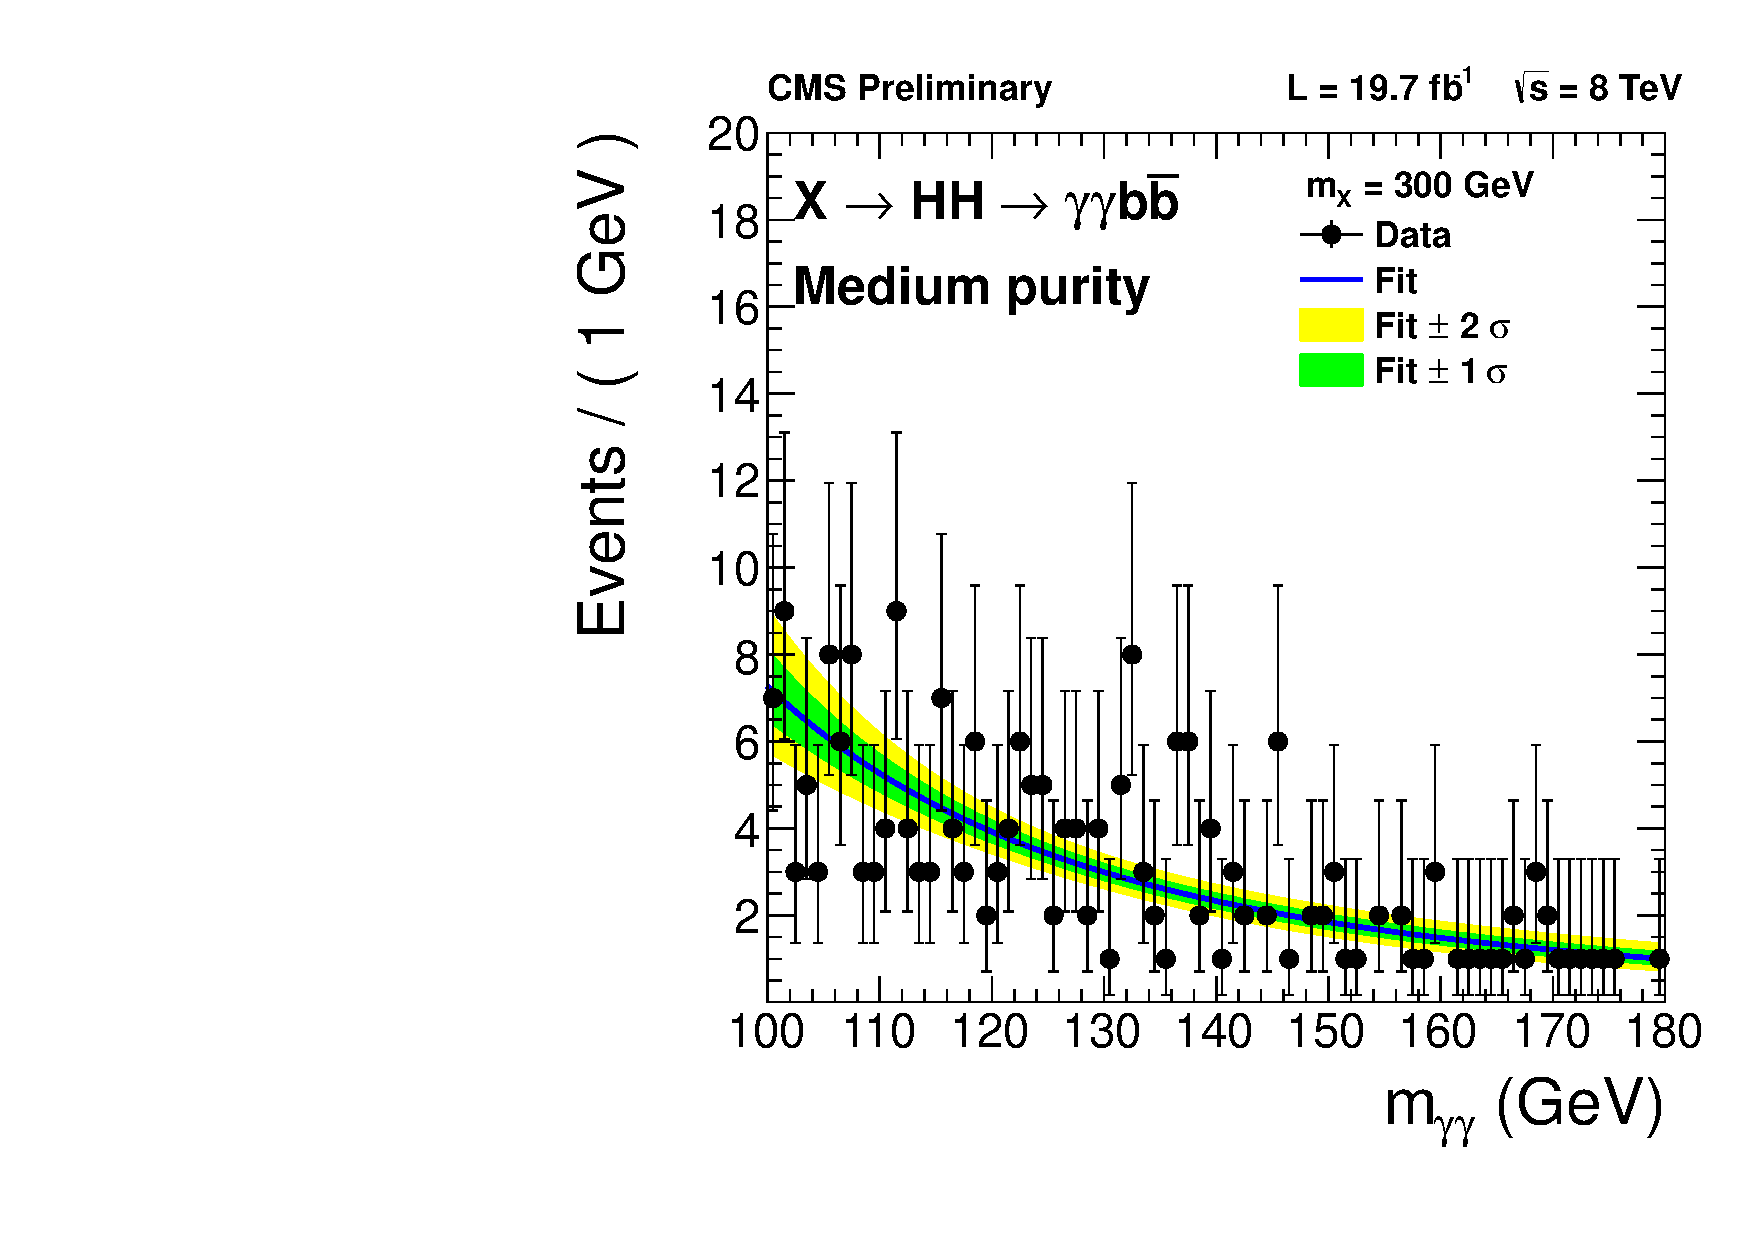
\includegraphics[width=0.45\textwidth]{figures/results/databkgoversig_cat1_300GeV.pdf}
   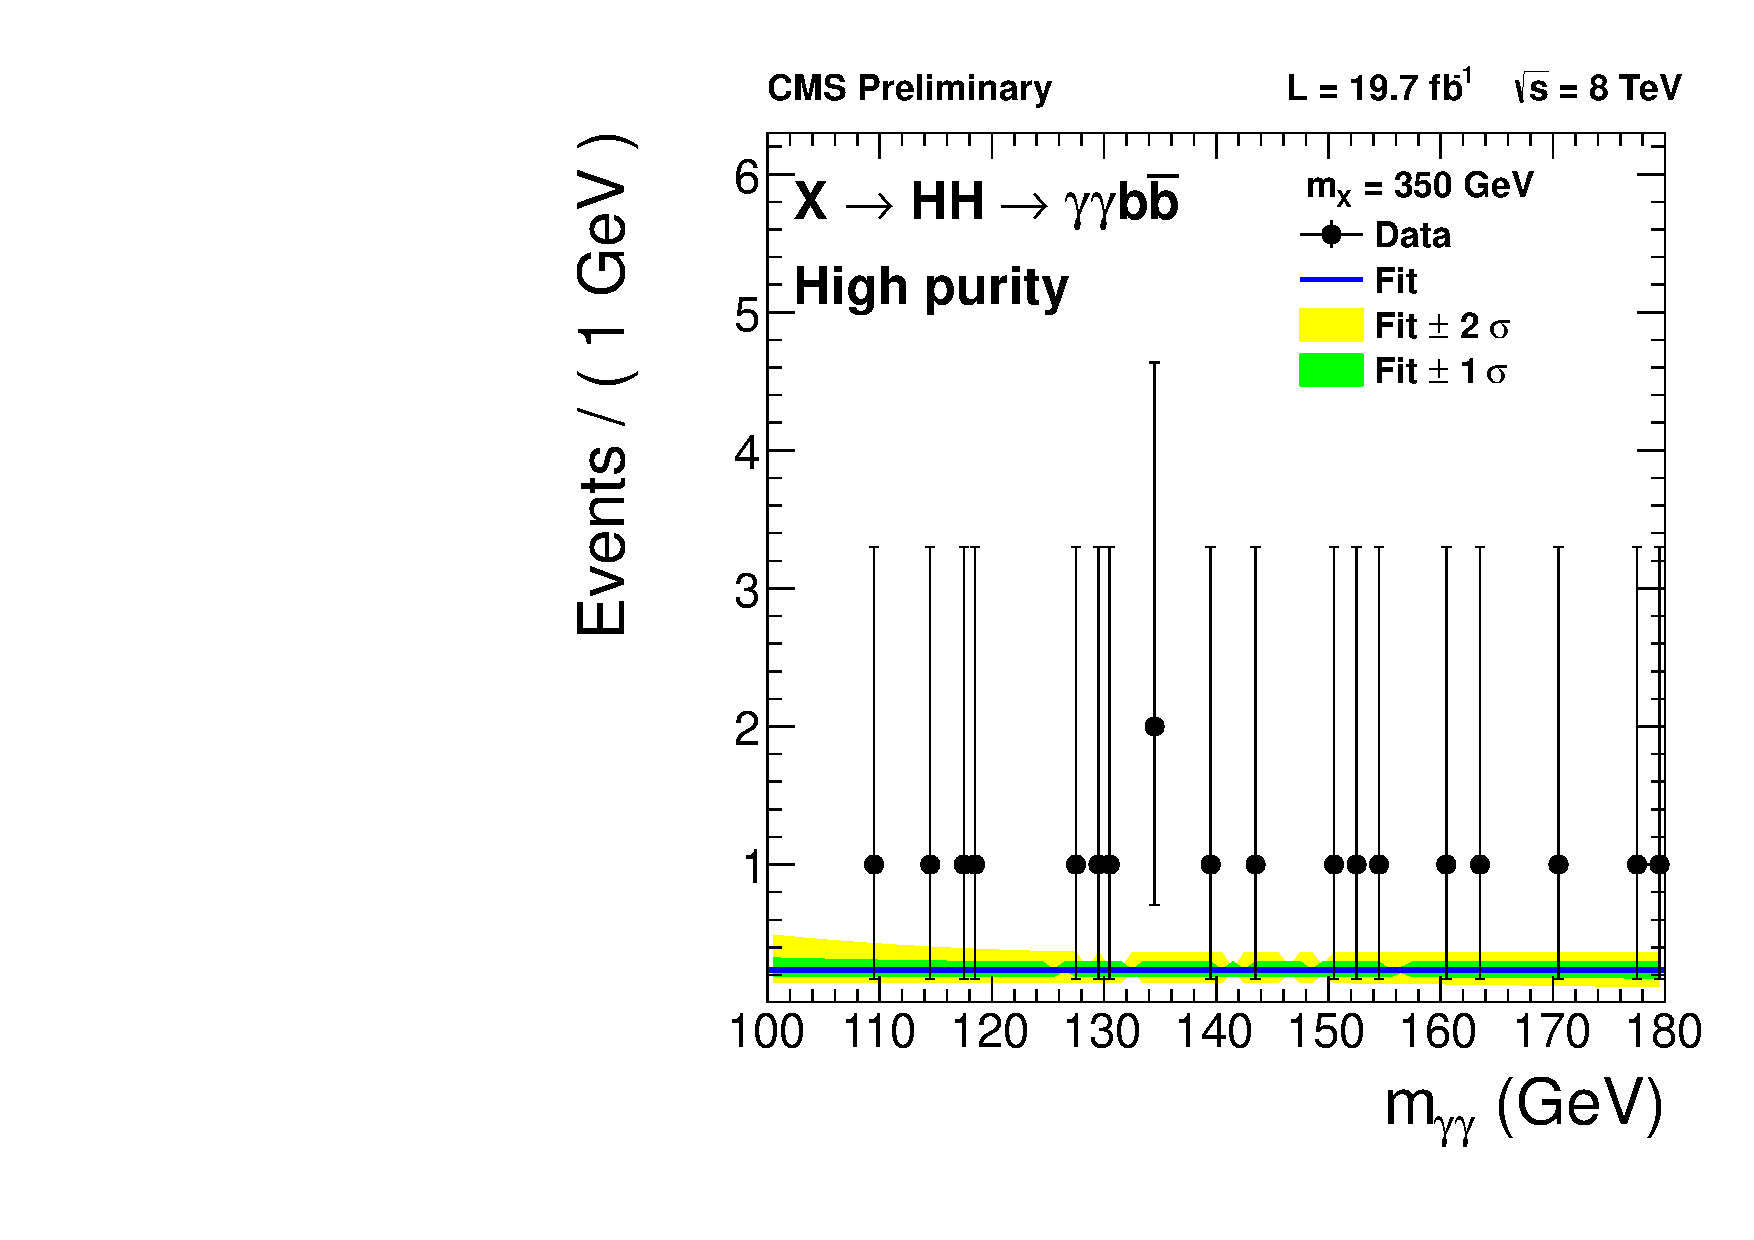
\includegraphics[width=0.45\textwidth]{figures/results/databkgoversig_cat0_350GeV.pdf}
   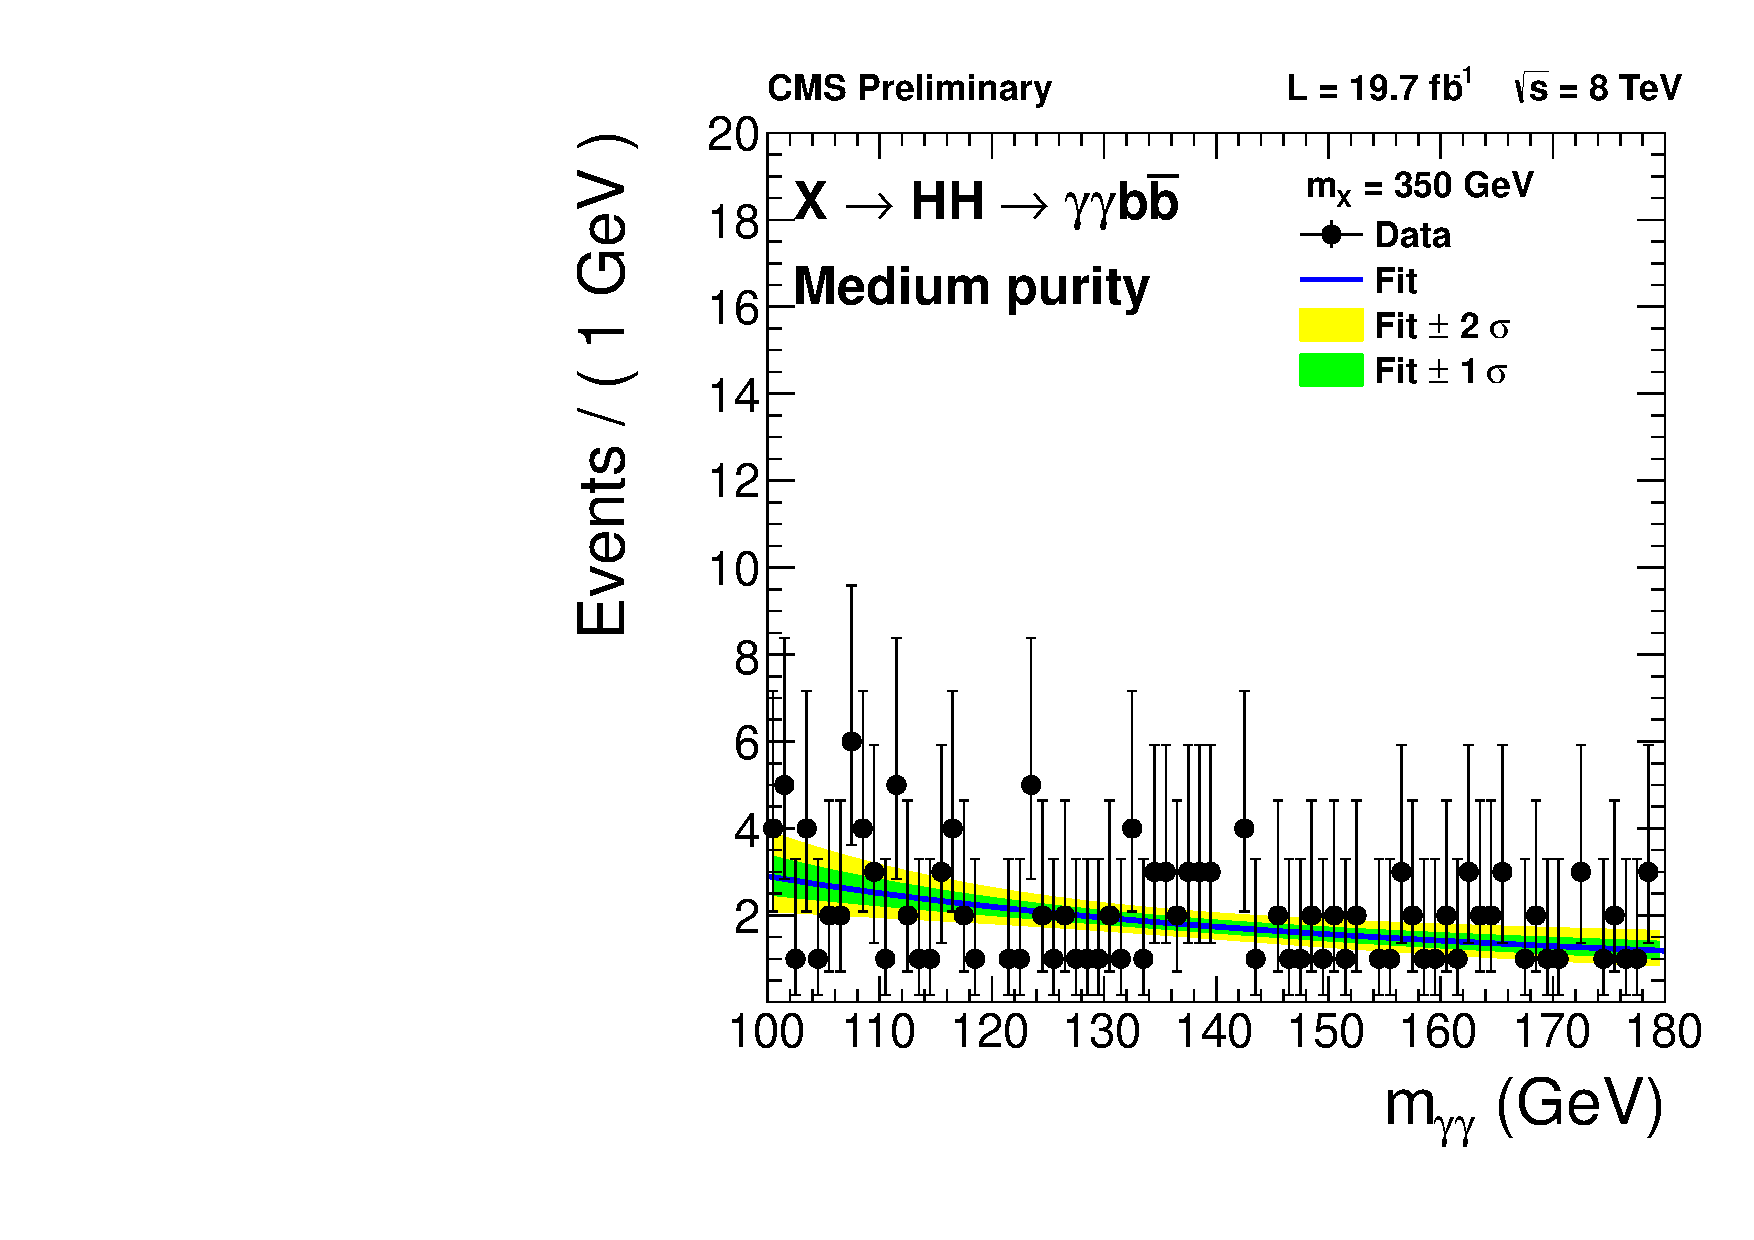
\includegraphics[width=0.45\textwidth]{figures/results/databkgoversig_cat1_350GeV.pdf}
 \end{center}
\caption{Events in the $\Mgg$ spectrum in the high-purity (left column) and medium-purity
(right column) categories for the resonance mass hypotheses 300 GeV (top row) and 350 GeV (bottom row)
The nonresonant component of the background fit is shown in blue
with its corresponding 1$\sigma$ and 2$\sigma$ confidence intervals.}
\label{fig:datafit_300}
\end{figure}

The background fit estimates only the nonresonant contribution arising from diphoton
production. The contribution from SM Higgs production with $\Hgg$ creates a resonance in the
spectrum that mimics the signal process. This resonant background
contribution is therefore added in the fit and accounted for in the limits.
The expected contribution of the resonant background is small, and the
effect on the final result is found to be at most 2\% for all low-mass resonant hypotheses.

No excess above the expectation is observed, so upper limits on the signal cross section are calculated.
The 95\% CL for observed and expected upper limits is shown in
Table~\ref{table:limits_lowmass} and Figure~\ref{fig:limits_lowmassres}
for both categories and for the high-purity category only.
The latter result is provided to simplify the comparison with new physics models where
the Higgs branching ratios for the $\Hgg$ and $\Hbb$ decays can be modified with respect to their
values in the SM.
The green and yellow bands represent the 1$\sigma$ and 2$\sigma$
confidence intervals around the expected limit. Theory expectations for Radion, RS1 KK-graviton, and 
bulk KK-graviton are shown, where the Radion expectation assumes $\text{BR}(R\rightarrow HH) =$~25\%
for all Radion masses above 300 GeV. Through comparison with the Graviton simulation,
the search is verified to be spin-independent, so theory expectations for both spin-0 and spin-2
hypotheses may be overlaid together.

\begin{table}[ht!]
  \centering
  \renewcommand{\arraystretch}{1.4}
  \caption{Observed and median expected 95\% CL upper limits for $m_X \le 400$~GeV.}
  \begin{tabular}{ | c || c | c || c | c |}
\hline
$m_X$ (GeV) & Observed limit (fb) & Expected limit (fb) & Observed limit (fb) & Expected limit (fb) \\ \hline
 & & &  \multicolumn{2}{c|}{High-purity category only} \\ \hline
260 & 3.14 & 2.12 & 3.54 & 2.41 \\
270 & 2.70 & 2.40 & 3.07 & 2.74 \\
300 & 3.98 & 2.73 & 3.64 & 3.14 \\
350 & 1.67 & 2.23 & 2.17 & 2.66 \\
400 & 1.97 & 1.66 & 3.40 & 2.01 \\ \hline
\end{tabular}

  \label{table:limits_lowmass}
\end{table}

\begin{figure}[ht!]
 \begin{center}
   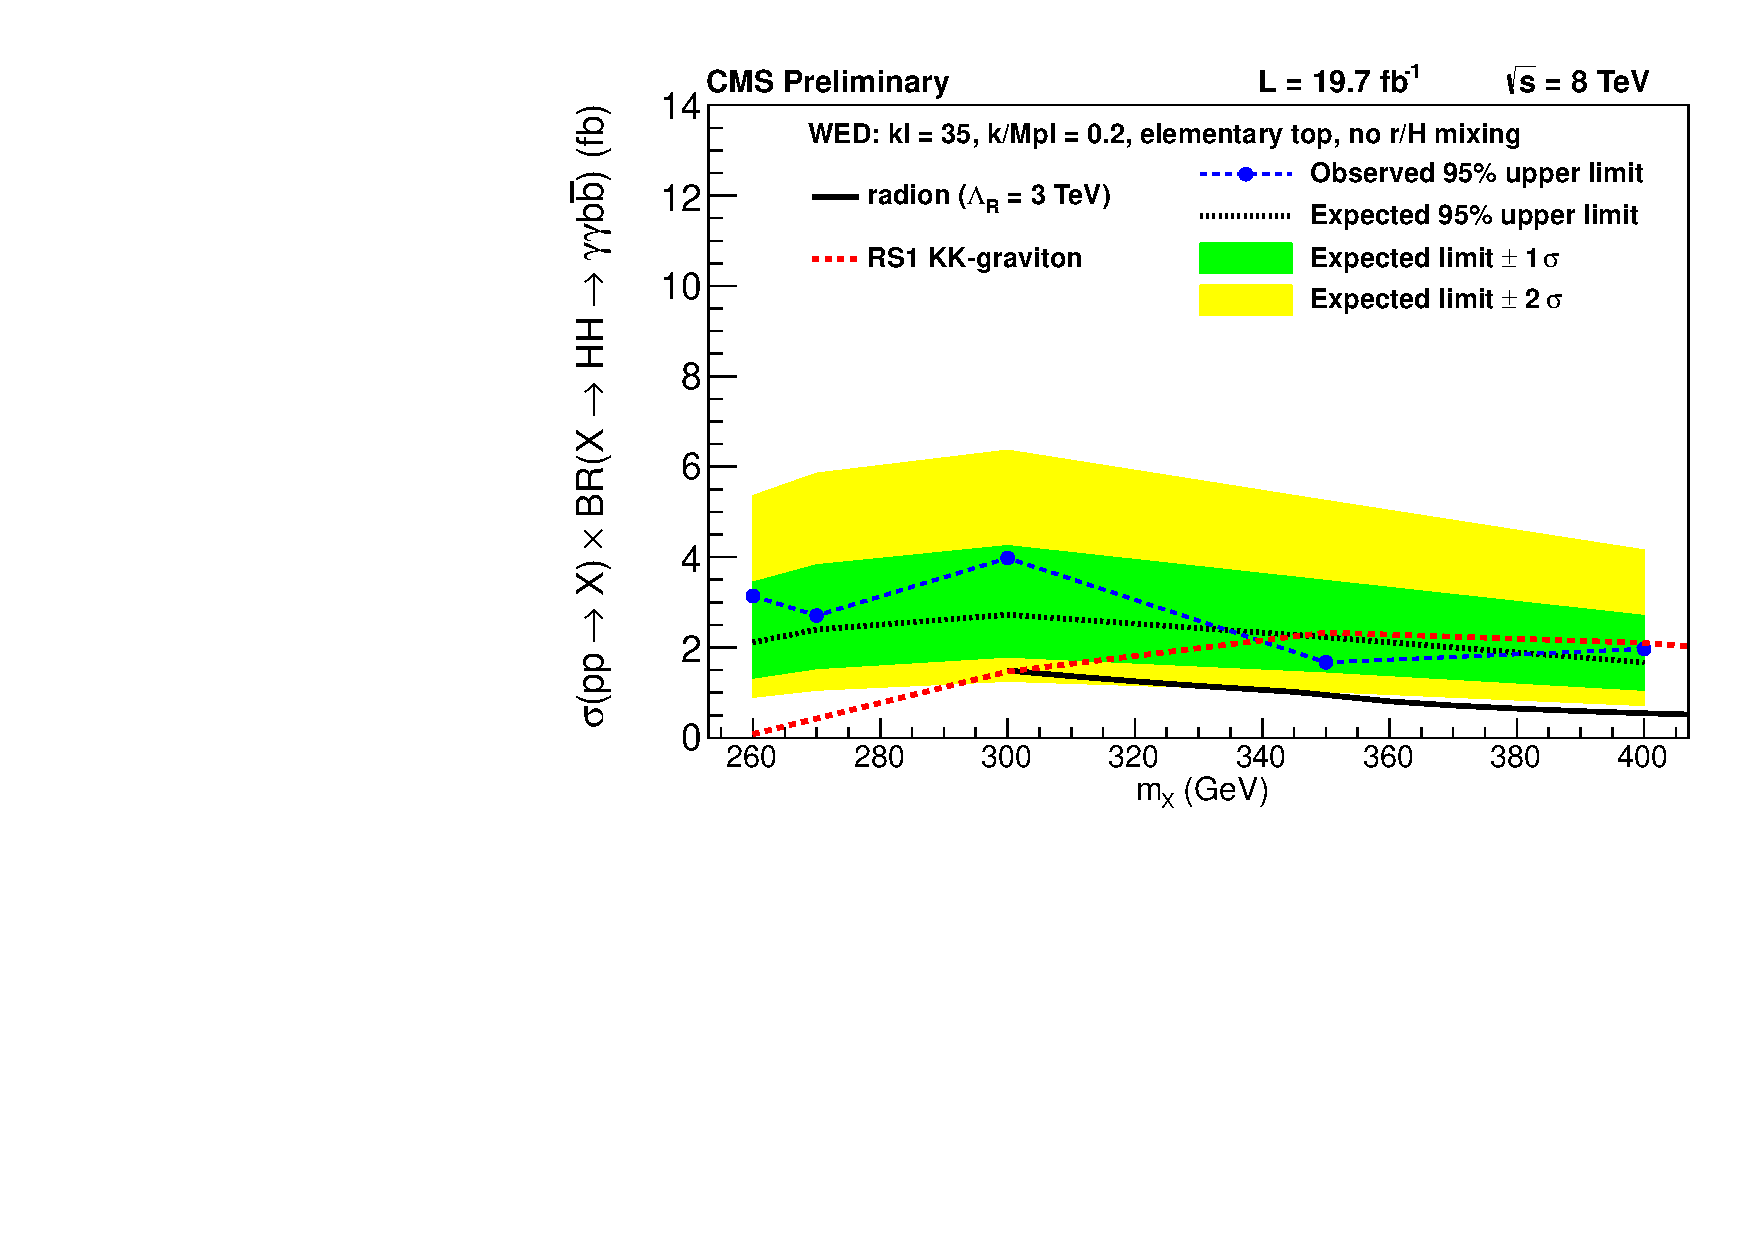
\includegraphics[width=0.7\textwidth]{figures/results/WP4_cutbased_low_all.pdf}
   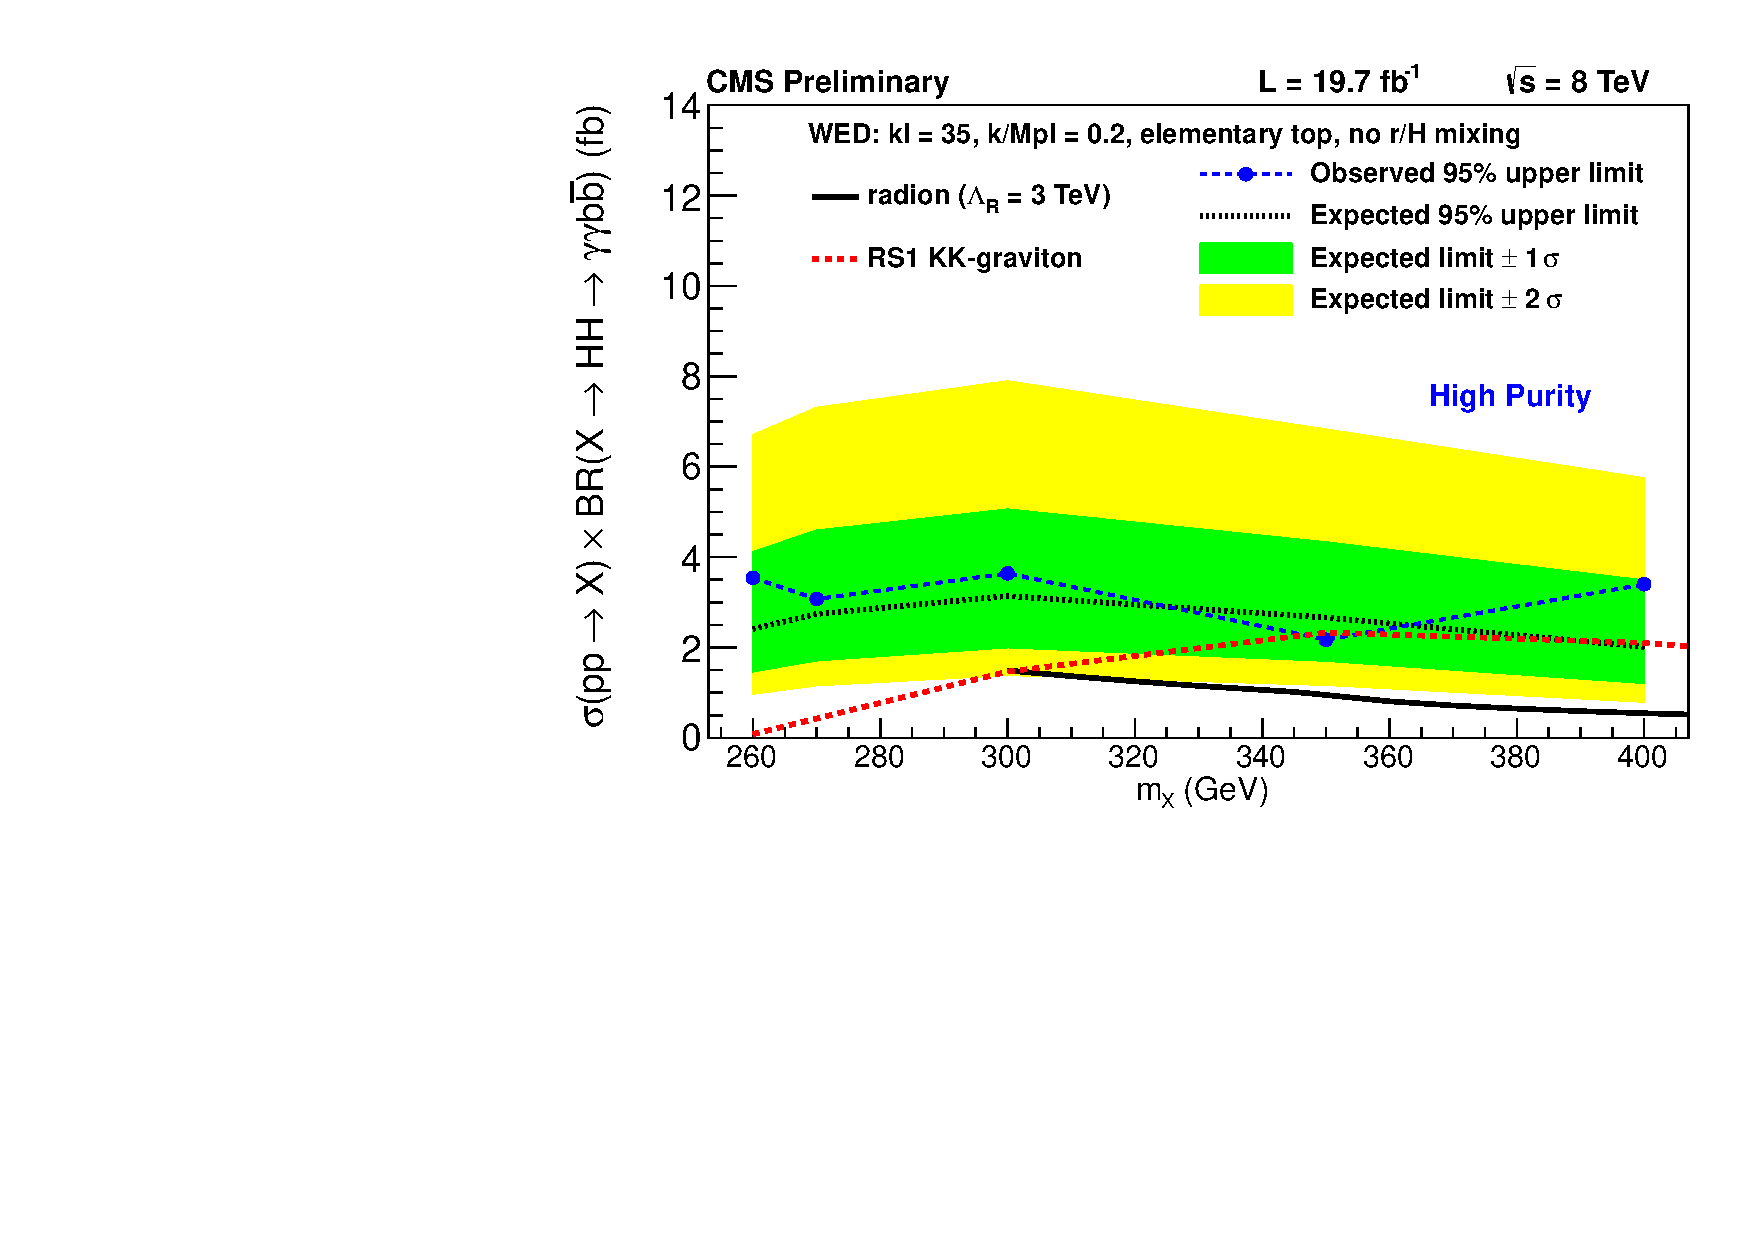
\includegraphics[width=0.7\textwidth]{figures/results/WP4_cutbased_low_base_onecat.pdf}
 \end{center}
\caption{Expected 95\% CL upper limits on the cross section times branching ratio
$\sigma(pp\rightarrow X) \times \text{BR}( X \rightarrow HH \rightarrow \gamma\gamma b\bar{b})$.
Theory lines corresponding to WED models with Radion, RS1 KK-graviton, and bulk KK-graviton are
overlaid. Limits from both categories (top) and high-purity category only (bottom) are shown.
The results are obtained using the asymptotic $\text{CL}_s$ approach.}
\label{fig:limits_lowmassres}
\end{figure}

\subsection{High-mass Resonant Results}

For the high-mass resonant search, the signal yield is extracted by fitting the $\Mggjjk$ spectrum
in a procedure similar to the one for the low-mass resonant search. The signal model is built
for each mass hypothesis by fitting the $\Mggjjk$ peak in the simulation sample separately for the
two categories. The functional form used is the sum of a Crystal Ball and Gaussian with each mean
constrained to be the same. The position of the peak follows the corresponding $m_X$
hypothesis closely,
and the resolution in the peak improves as $m_X$ increases. Figure~\ref{fig:sigfit_500_1000}
shows examples of the signal fit for mass hypotheses of 500 GeV and 1 TeV.

\begin{figure}[ht!]
 \begin{center}
   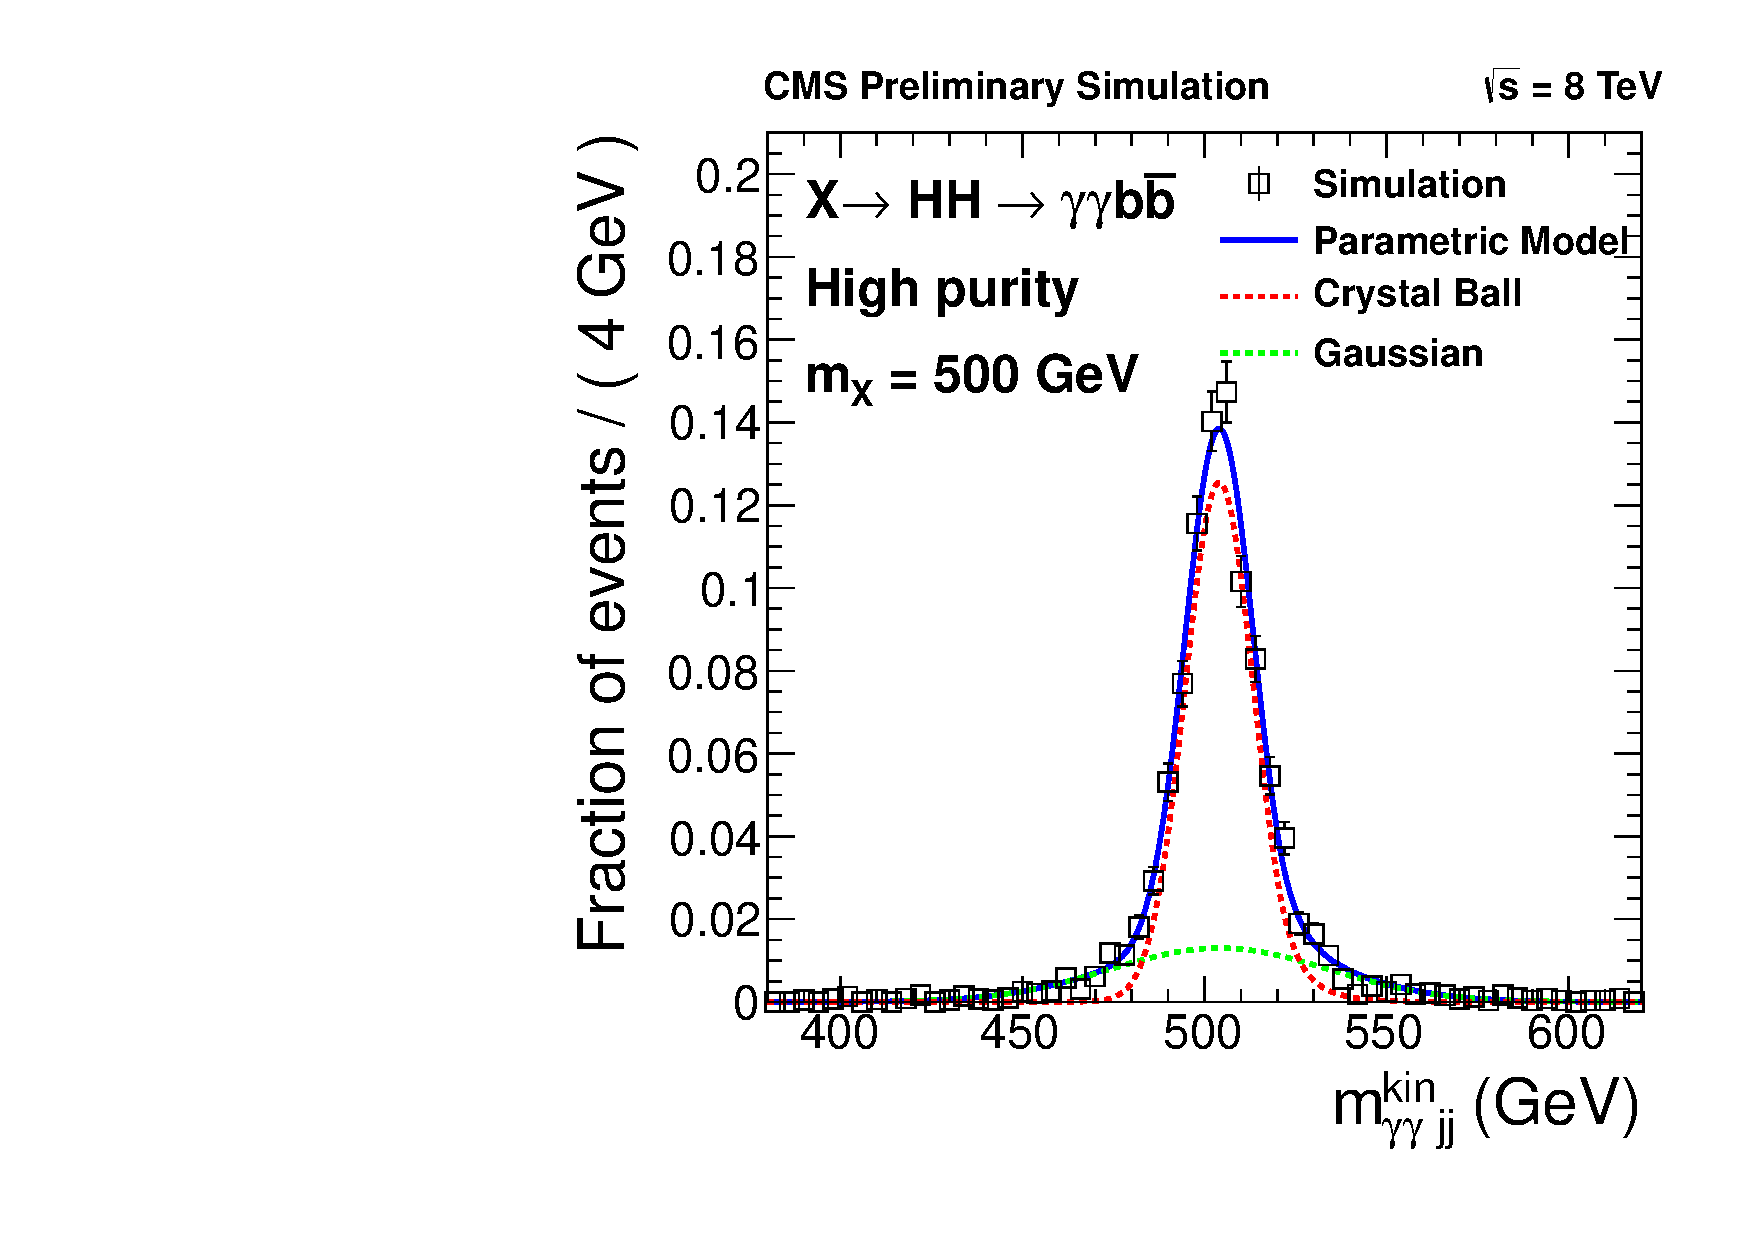
\includegraphics[width=0.45\textwidth]{figures/results/sigmodel_cat0_500GeV.pdf}
   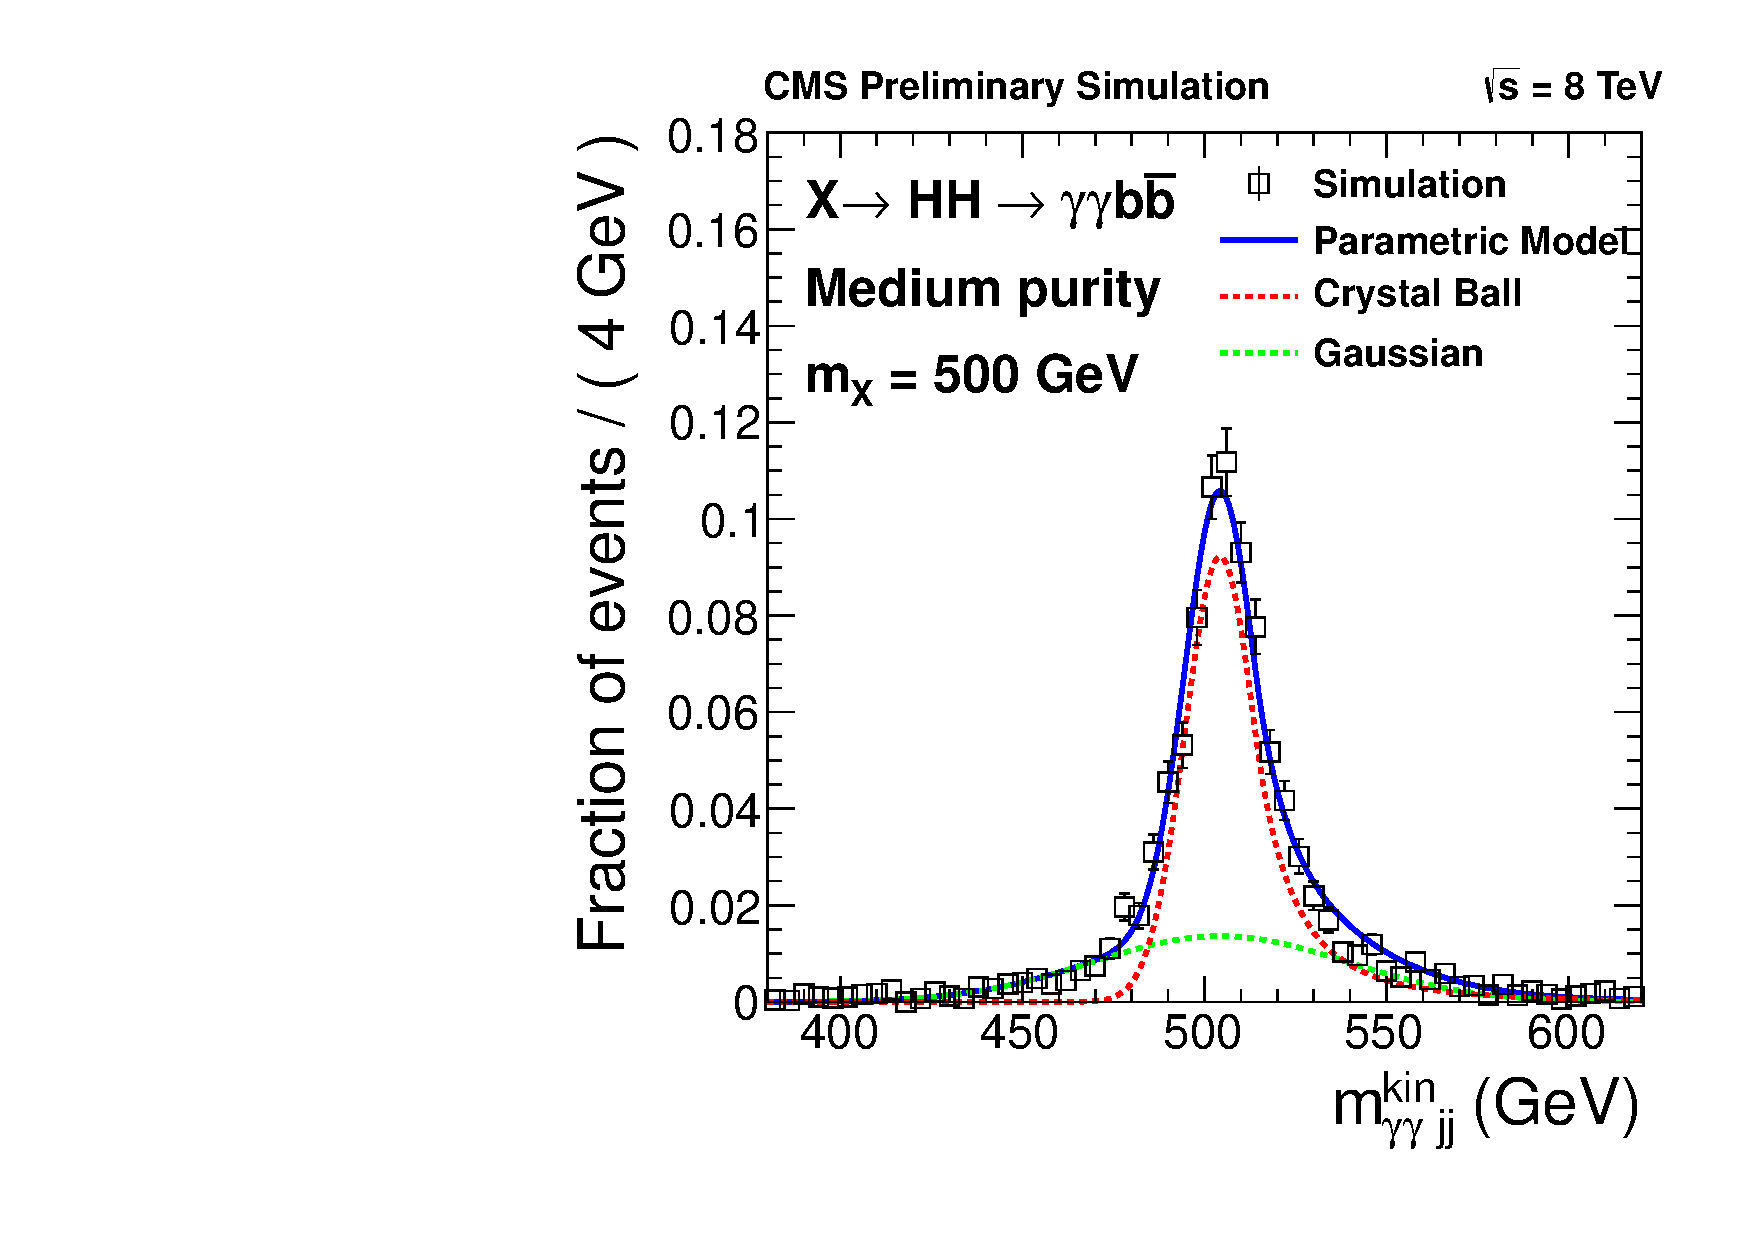
\includegraphics[width=0.45\textwidth]{figures/results/sigmodel_cat1_500GeV.pdf}
   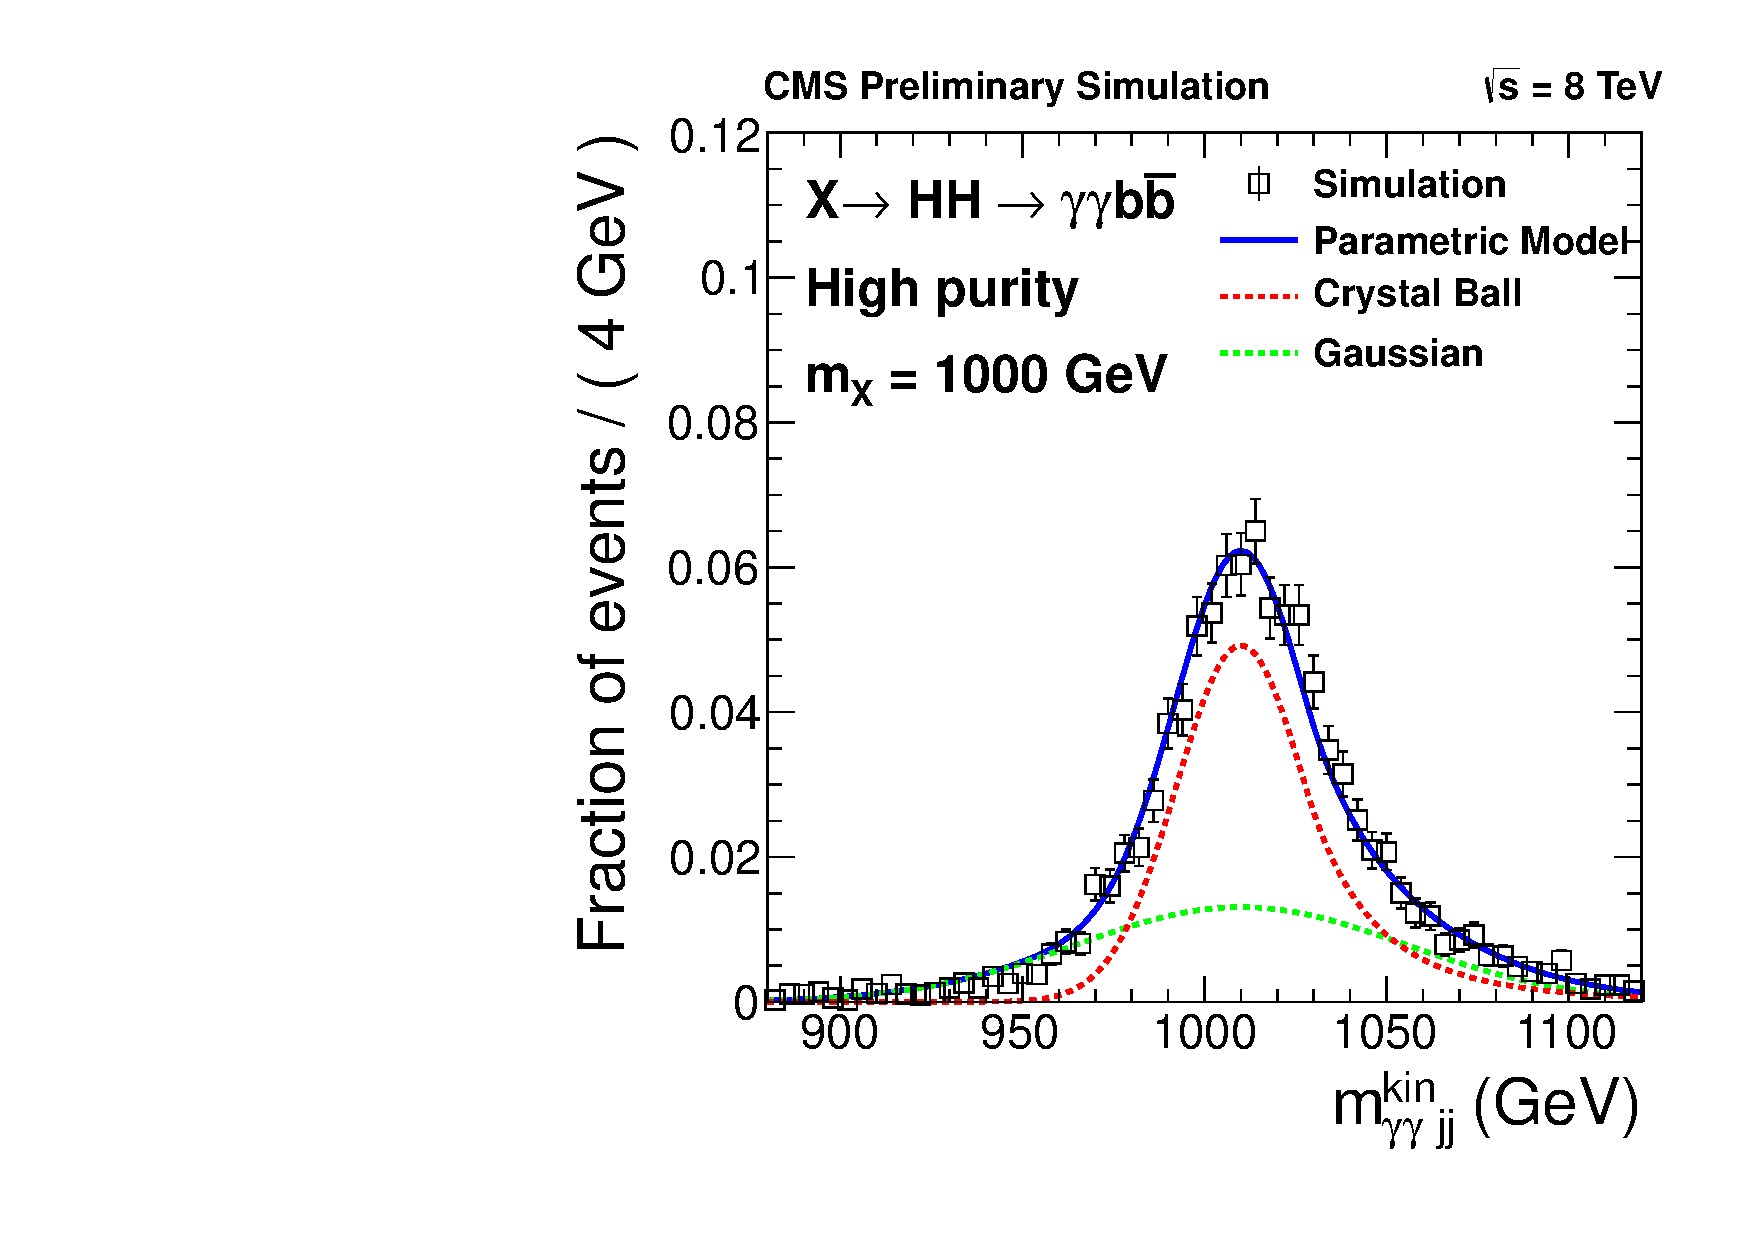
\includegraphics[width=0.45\textwidth]{figures/results/sigmodel_cat0_1000GeV.pdf}
   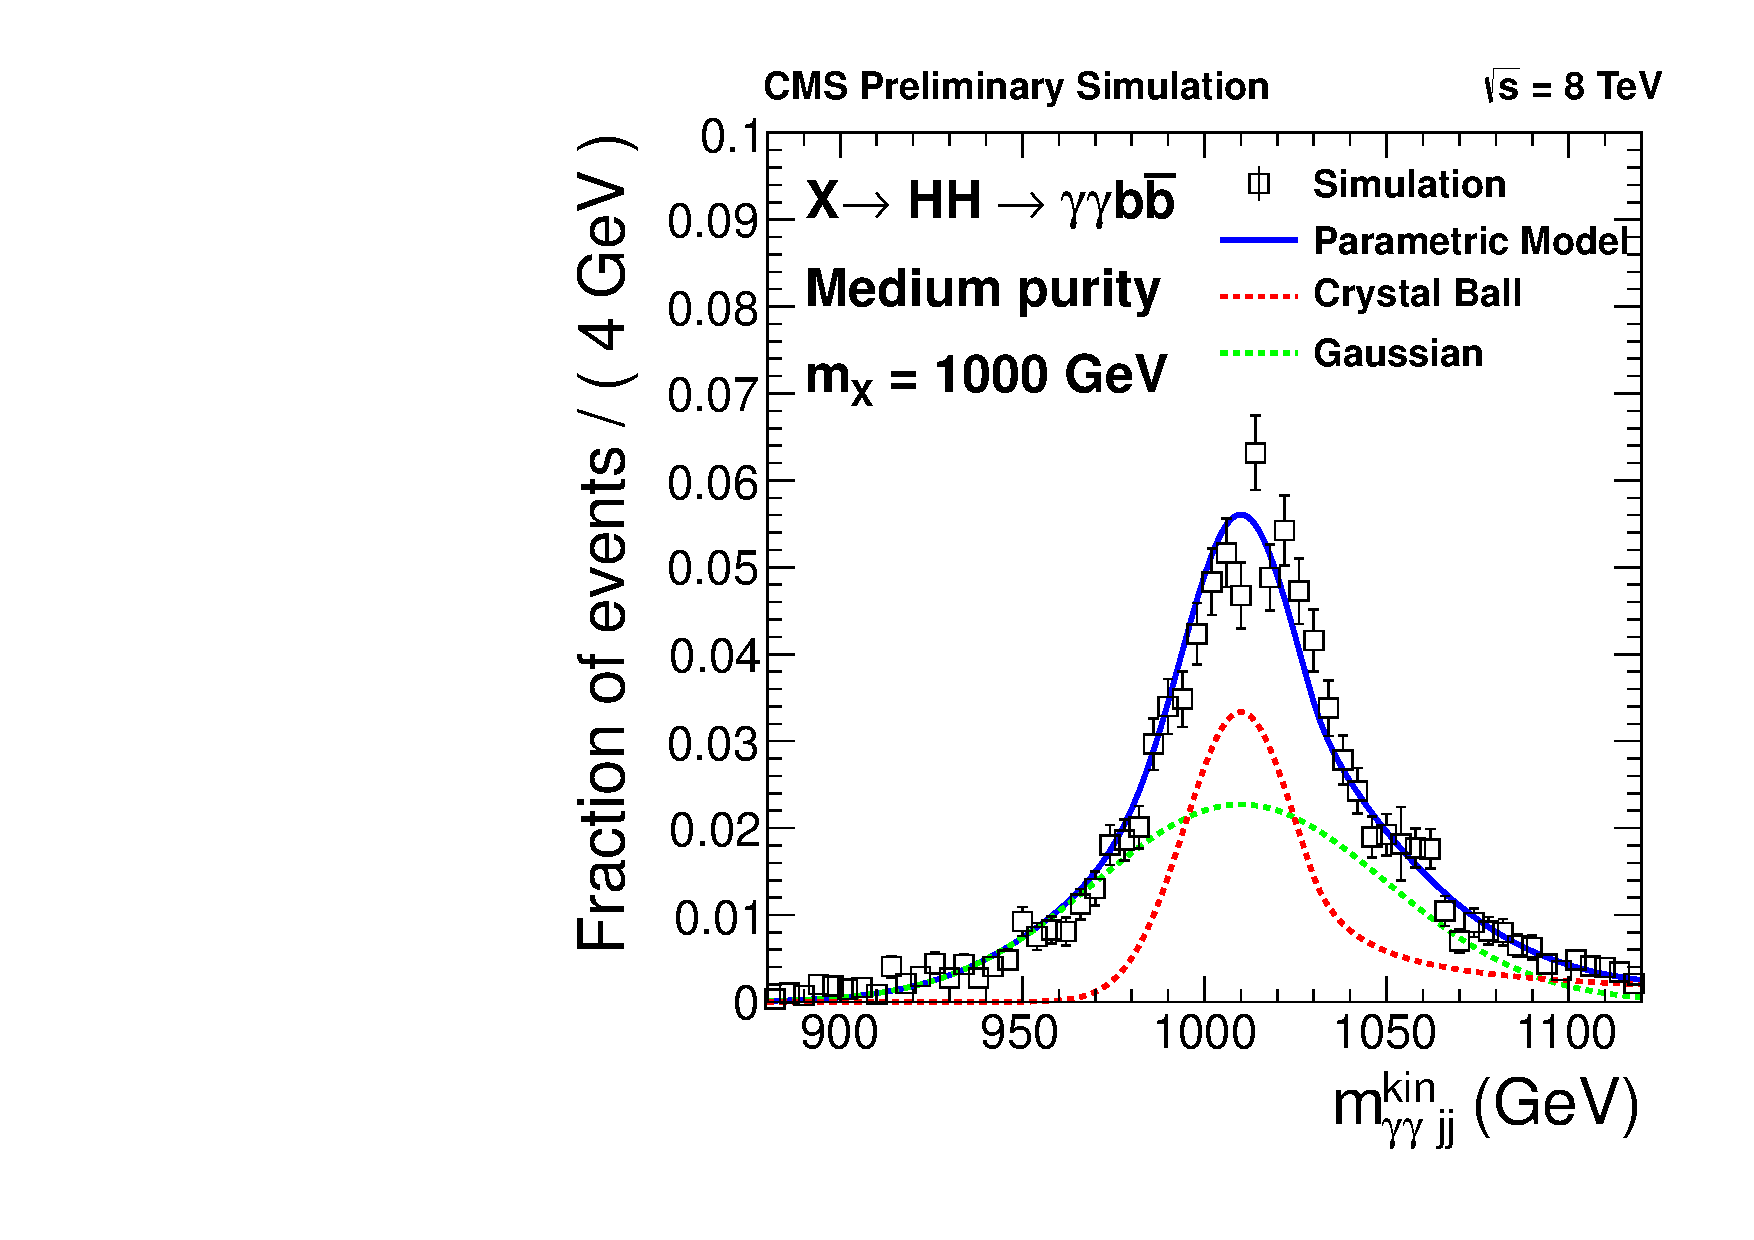
\includegraphics[width=0.45\textwidth]{figures/results/sigmodel_cat1_1000GeV.pdf}
 \end{center}
\caption{Simulated signal shape in the $\Mggjjk$ spectrum for the high-purity (left column)
and medium-purity (right column) categories for the Radion with mass 500 GeV (top row) and
1 TeV (bottom row). The open squares and corresponding
statistical uncertainties represent the simulation.
The blue line represents the signal model fitted to the simulation, while the green dashed line
and the red dashed line represent the two components of the signal model.}
\label{fig:sigfit_500_1000}
\end{figure}


The background estimation is done by fitting the same distribution in each category on the interval
$[320, 1200]$~GeV. The lower edge is chosen to avoid the kinematic turn-on of the background
while ensuring full containment of the 400 GeV signal. The same bias estimation procedure
described for the low-mass resonant search is applied here. The chosen background function is a power
law for both categories, shown in Figure~\ref{fig:datafit_4body}. Note that in this regime,
the SM Higgs background does not have a resonance on the $\Mggjjk$ spectrum, so
there is no resonant contamination from the background.

\begin{figure}[ht!]
 \begin{center}
   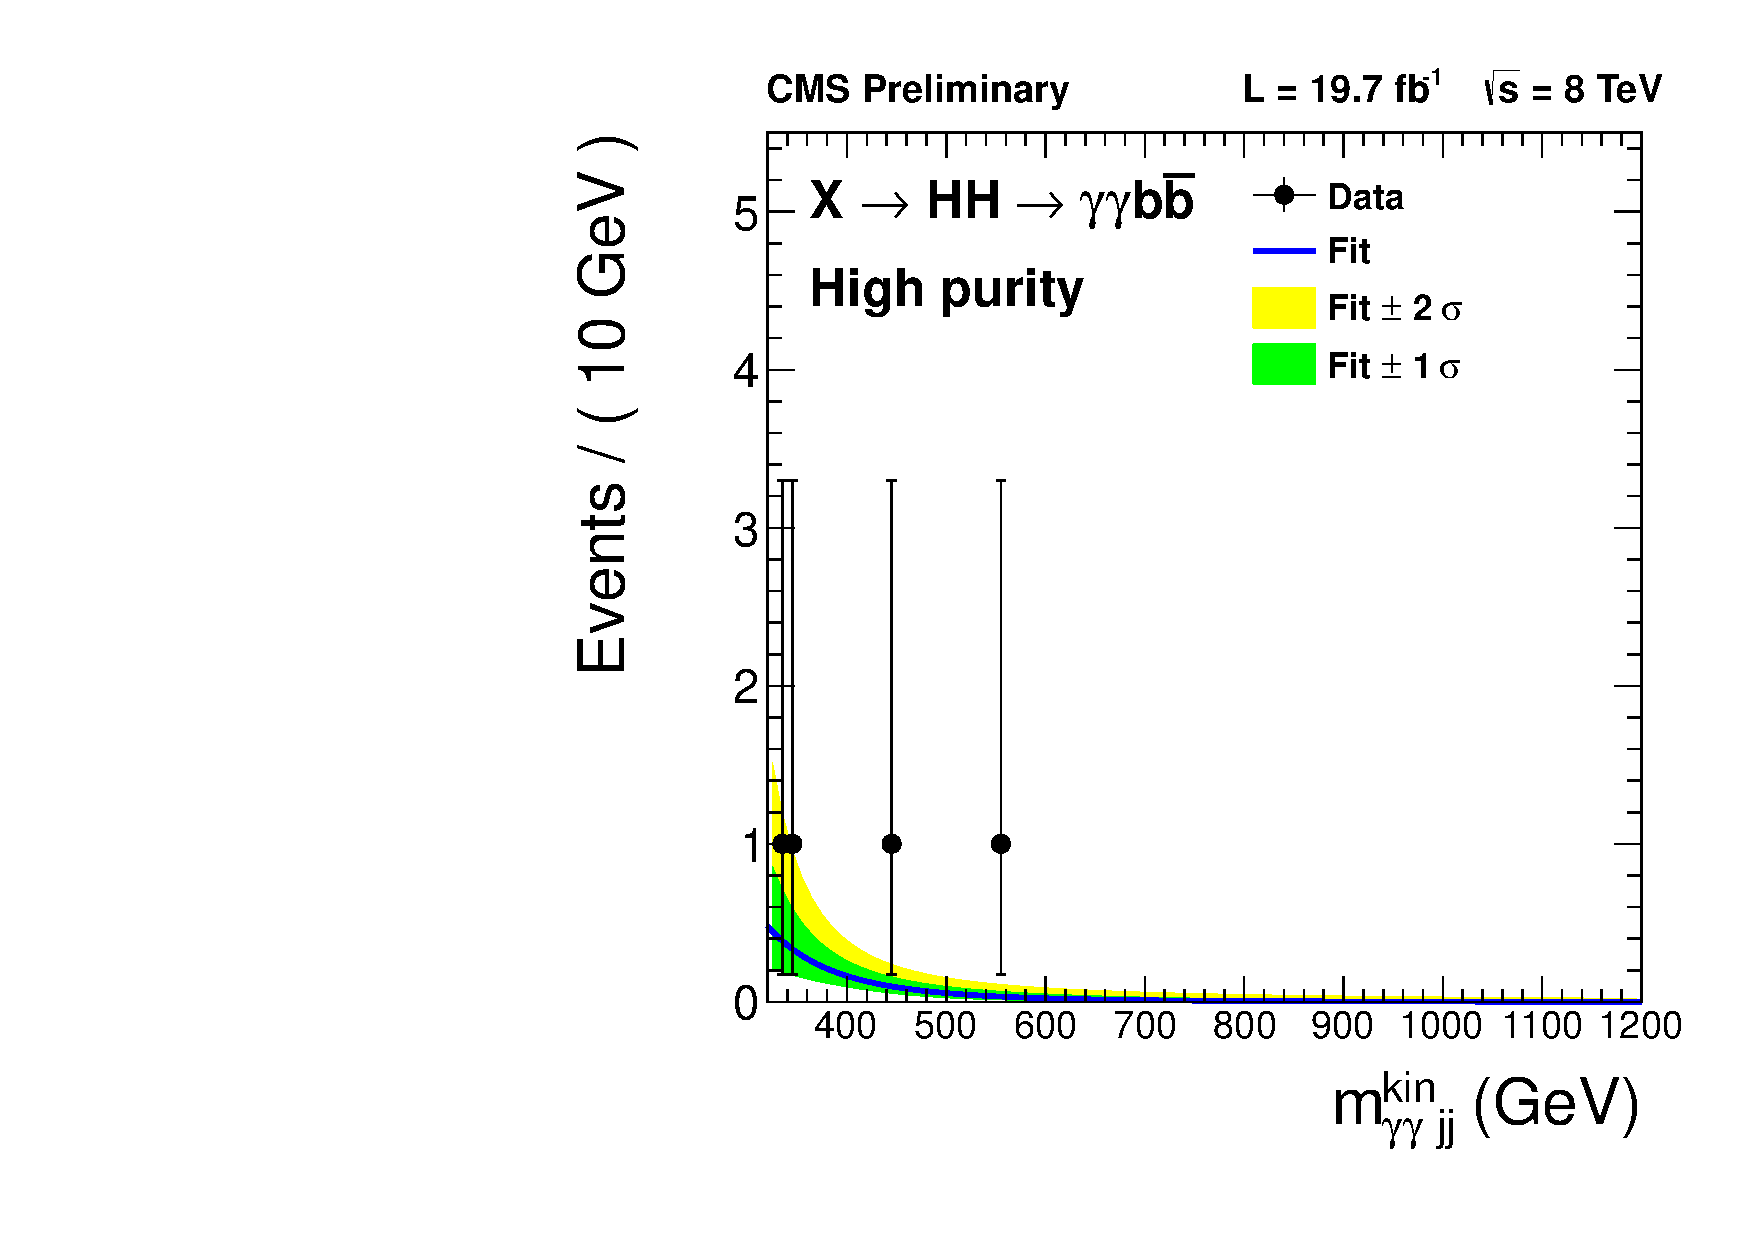
\includegraphics[width=0.45\textwidth]{figures/results/databkgoversig_cat0_4body.pdf}
   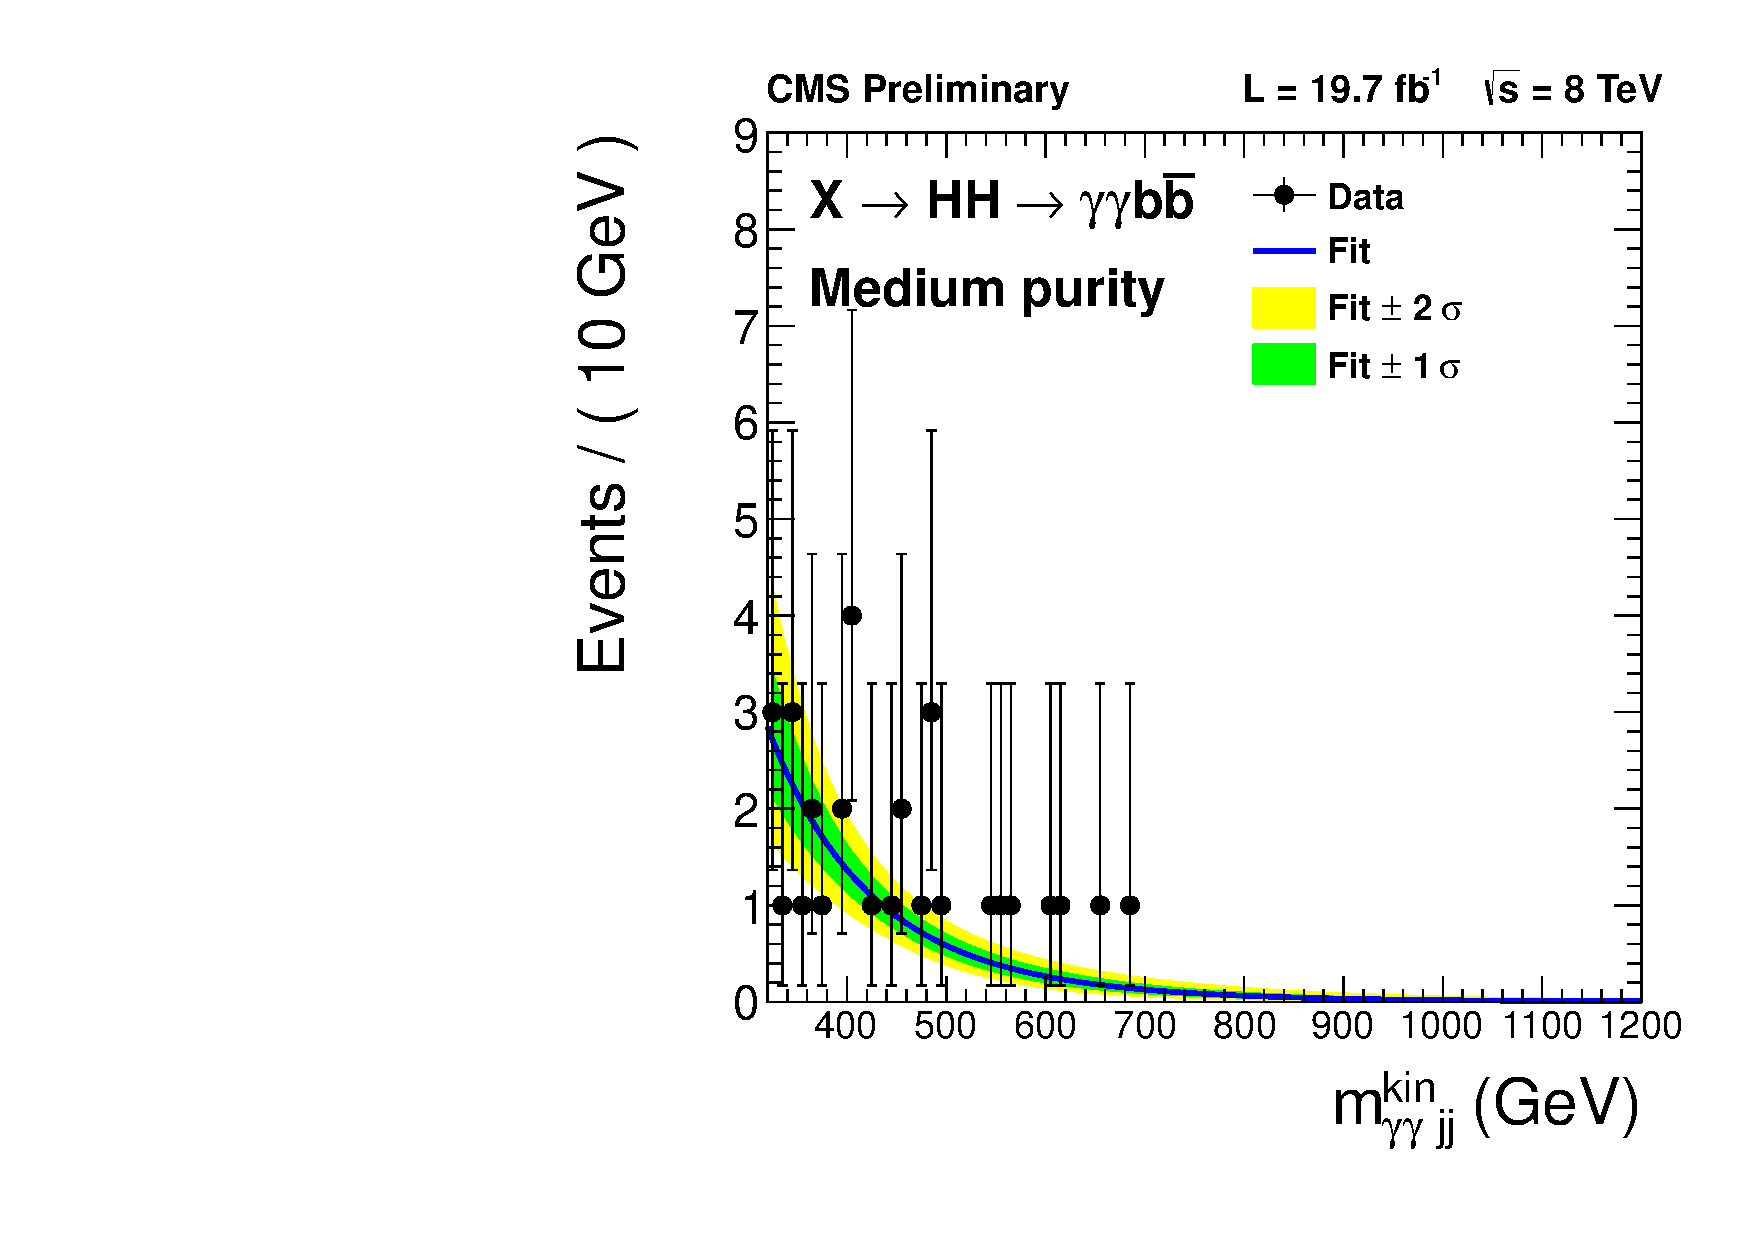
\includegraphics[width=0.45\textwidth]{figures/results/databkgoversig_cat1_4body.pdf}
 \end{center}
\caption{Events in the $\Mggjjk$ spectrum in the high-purity (left) and medium-purity (right)
categories. The background fit is shown in blue
with its corresponding 1$\sigma$ and 2$\sigma$ confidence intervals.}
\label{fig:datafit_4body}
\end{figure}

No excess above the expectation is observed, so upper limits on the signal cross section are calculated.
The 95\% CL for expected and observed limits is
shown in Table~\ref{table:limits_highmass} and Figure~\ref{fig:limits_allres}.
The break at 400 GeV corresponds
to the border between the two methods for signal extraction.
As in the low-mass regime, the theory expectations for the Radion assumes
$\text{BR}(R\rightarrow HH) =$~25\% for all Radion masses above 300 GeV. The result is again
spin-independent, allowing for both spin-0 and spin-2 theory expectations to be overlaid together.

\begin{table}[ht!]
  \centering
  \renewcommand{\arraystretch}{1.4}
  \caption{Observed and median expected 95\% CL upper limits for $m_X \ge 400$~GeV.}
  \begin{tabular}{ | c | c | c | }
\hline
$m_X$ (GeV) & Observed limit (fb) & Expected limit (fb) \\ \hline
400 & 2.98 & 1.87 \\
450 & 1.76 & 1.42 \\
500 & 1.19 & 0.97 \\
550 & 1.45 & 0.80 \\
600 & 0.98 & 0.69 \\
650 & 0.61 & 0.60 \\
700 & 0.44 & 0.54 \\
800 & 0.31 & 0.46 \\
900 & 0.32 & 0.43 \\
1000 & 0.33 & 0.43 \\
1100 & 0.41 & 0.48 \\ \hline
\end{tabular}

  \label{table:limits_highmass}
\end{table}

\begin{figure}[ht!]
 \begin{center}
   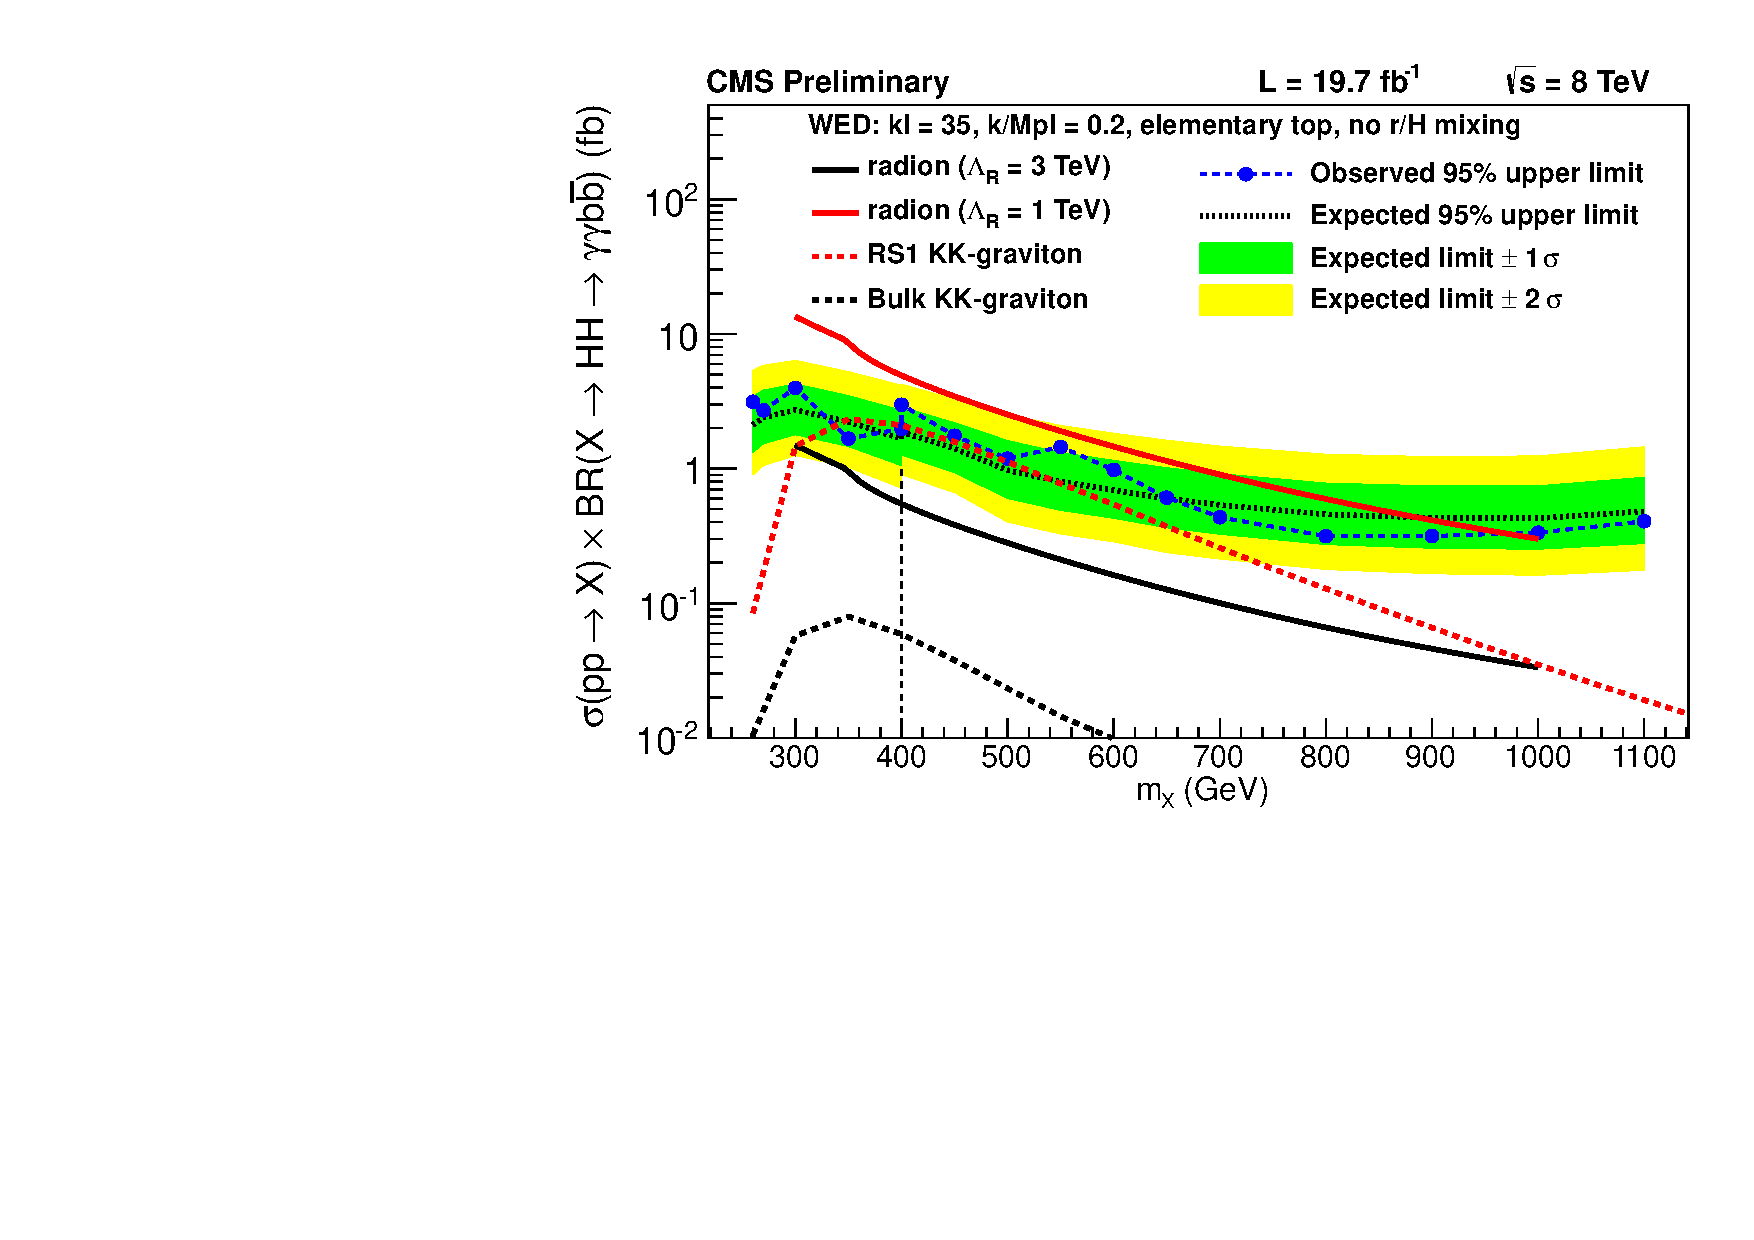
\includegraphics[width=0.7\textwidth]{figures/results/WP4_cutbased_all.pdf}
   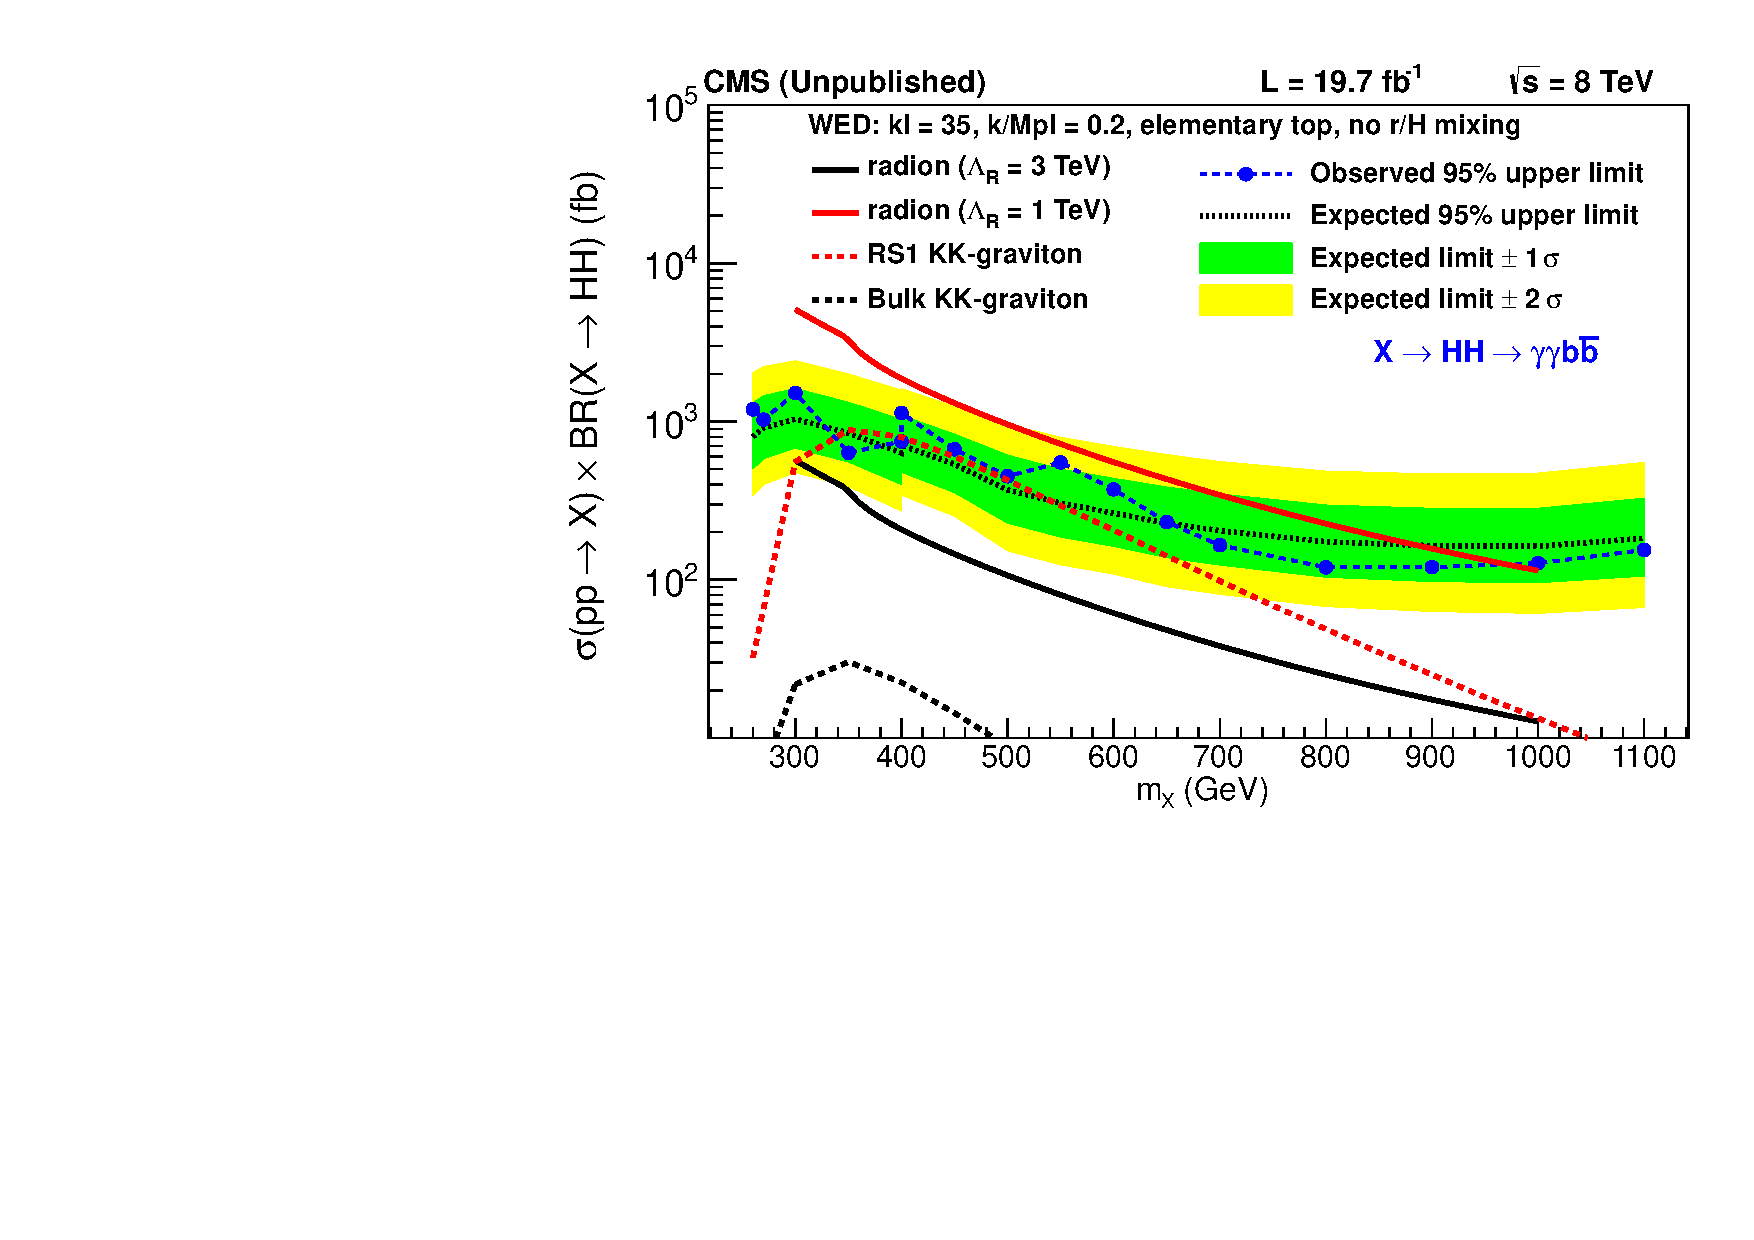
\includegraphics[width=0.7\textwidth]{figures/results/WP4_cutbased_HH.pdf}
 \end{center}
\caption{Expected 95\% CL upper limits on the cross section times branching ratios
$\sigma(pp\rightarrow X) \times \text{BR}( X \rightarrow HH \rightarrow \gamma\gamma b\bar{b})$ (top)
and $\sigma(pp\rightarrow X) \times \text{BR}( X \rightarrow HH )$ (bottom).
Theory lines corresponding to WED models with Radion, RS1 KK-graviton, and bulk KK-graviton are
overlaid. The results are obtained using the asymptotic $\text{CL}_s$ approach.}
\label{fig:limits_allres}
\end{figure}

Figure~\ref{fig:limit_comp} provides a comparison of the observed and expected limits obtained
among several final states in both the CMS and ATLAS Collaborations. The final states compared here
are $\gamma \gamma b\bar{b}$, $b\bar{b}b\bar{b}$, $\tau\tau b\bar{b}$, and multileptons and photons.
The comparison reveals that the $\gamma \gamma b\bar{b}$ is most sensitive to resonant double
Higgs production for $m_X < 400$~GeV, while the $b\bar{b}b\bar{b}$ final state is the most sensitive
for $m_X > 400$~GeV.

\begin{figure}[ht!]
 \begin{center}
   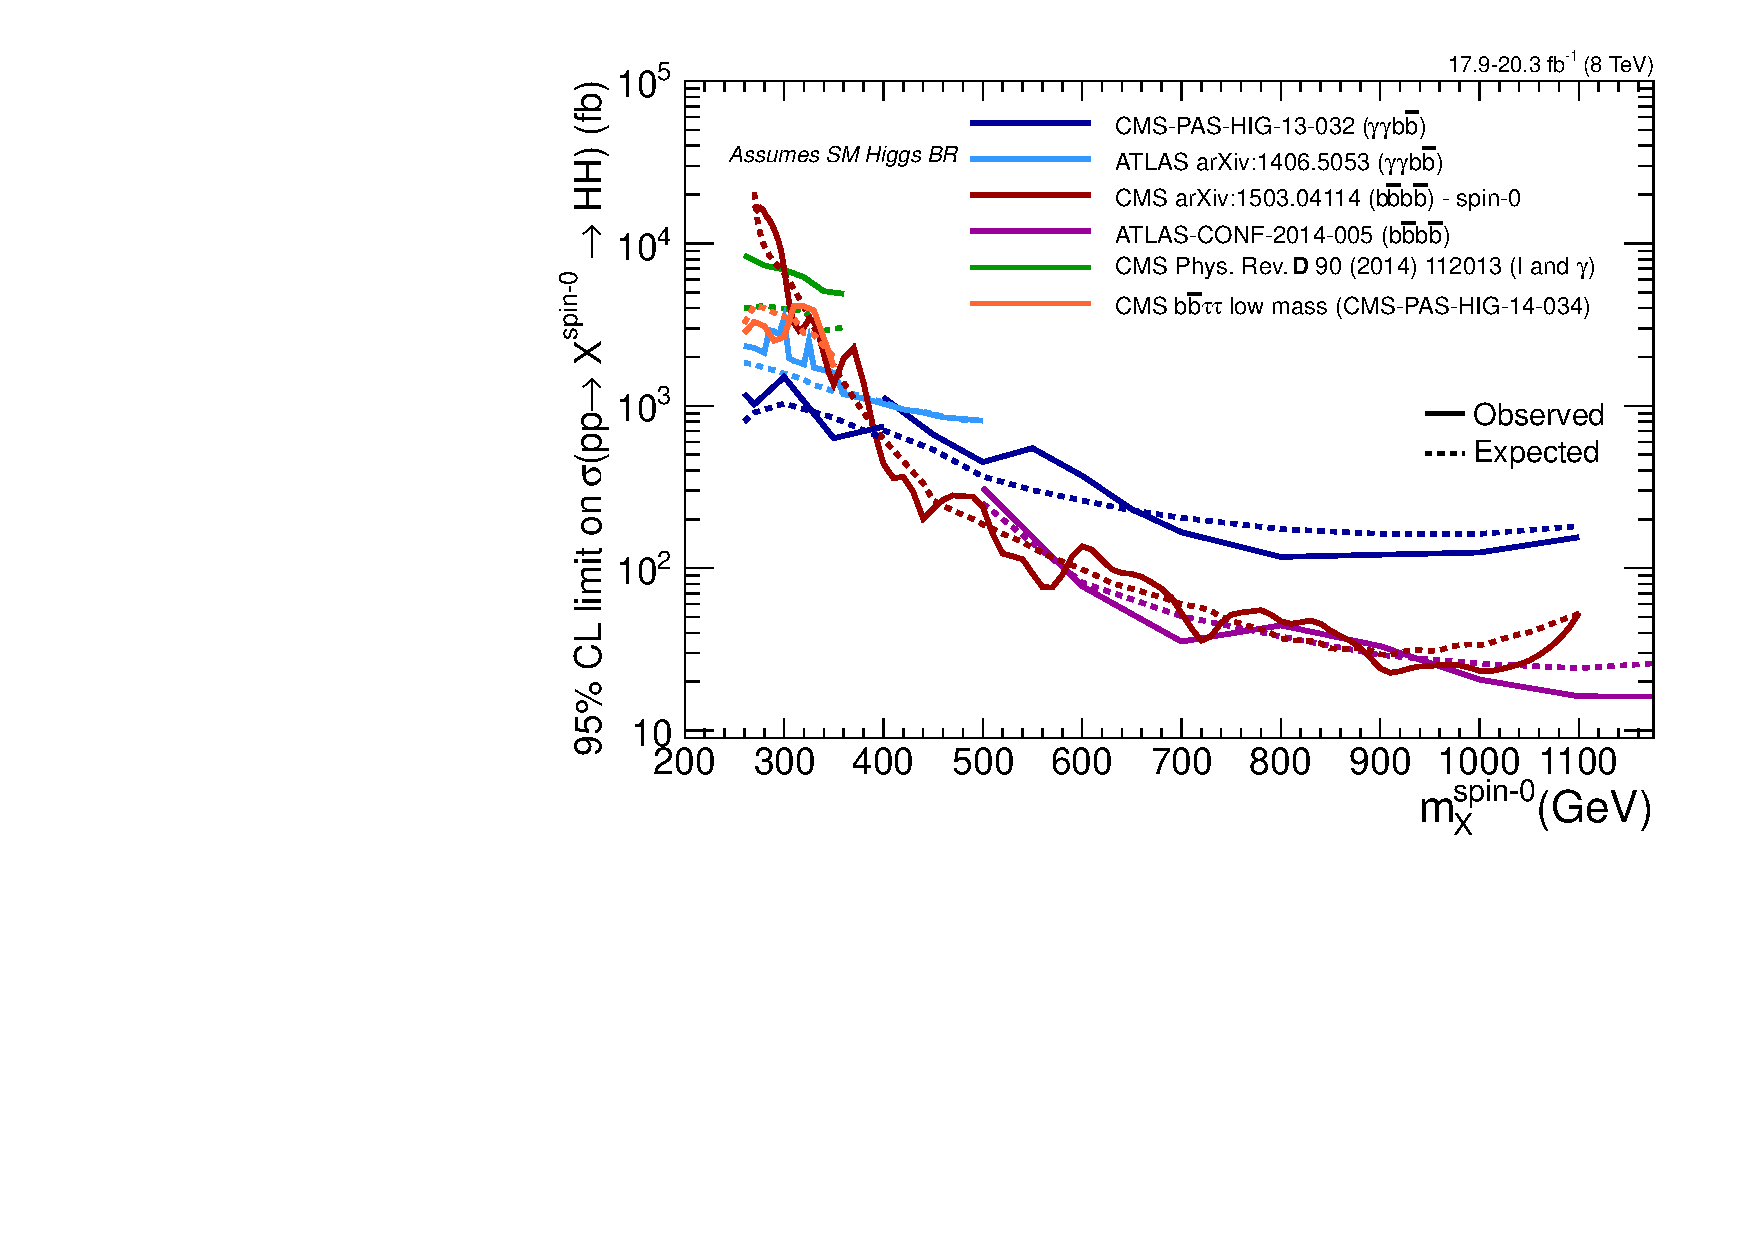
\includegraphics[width=0.8\textwidth]{figures/results/limit_comparison_all.pdf}
 \end{center}
\caption{The observed and expected upper limits of $X_\text{spin-0} \rightarrow HH$ production
at 95\% CL are compared over various searches performed by the CMS and ATLAS Collaborations
looking at the $\gamma \gamma b\bar{b}$~\cite{CMS-PAS-HIG-13-032,Aad:2014yja},
$b\bar{b}b\bar{b}$~\cite{Khachatryan:2015yea,ATLAS-CONF-2014-005},
$\tau\tau b\bar{b}$~\cite{CMS-PAS-HIG-14-034}, and
multileptons and photons~\cite{PhysRevD.90.112013}
final states. As the CMS $b\bar{b}b\bar{b}$ result is dependent on the
resonance spin, the spin-0 result for that analysis is used.}
\label{fig:limit_comp}
\end{figure}


\section{Nonresonant Results\label{sec:nonresresults}}

For the SM nonresonant search, the signal yield is extracted by fitting the 2D plane
$\Mgg \times \Mjj$. The signal model is built by simultaneously fitting both dimensions
for each of the four categories separately. The functional form used in both dimensions is the sum of a Crystal Ball and
Gaussian with each mean constrained to be the same. The background estimation is done by fitting
the same plane in each category on the interval $[100, 180]$~GeV for $\Mgg$ and $[60, 180]$~GeV
for $\Mjj$. The same bias estimation procedure
described for the low-mass resonant search is applied here. The chosen background function is a power
law for both dimensions in all four categories. The SM Higgs production is treated as a resonant
background, and its contribution on the final result is a few percent.

No excess above the expectation is observed, so an upper limit on the signal cross section is
calculated. The 95\% CL is found using the same approach as in both
regimes of the resonant search. The observed (expected) upper limit on the SM
$pp \rightarrow HH \rightarrow \ggbb$ production cross section is 1.91 fb (1.59 fb).
Assuming SM Higgs branching ratios, the observed (expected) upper limit on SM $pp \rightarrow HH$
production is 726 fb (604 fb). In terms of the SM signal strength modificator $\mu_{HH}$, defined
generally as
\begin{equation}
\mu = \frac{\sigma}{\sigma_\text{SM}} \, ,
\end{equation}
the observed (expected) limit is 72.9 (60.7). These calculations account for the theoretical
uncertainty associated with the SM NNLO cross section.

%\section{The Future\label{sec:future}}



\chapter{Conclusion\label{ch:conclusion}}

Some rehash of abstract and intro



\appendix % all chapters following will be labeled as appendices
%\chapter{Mom, this is for you.\label{ch:mom}}

Explain the work of this thesis to my mom and anybody else.

%\chapter{Other Projects\label{ch:pastwork}}

\section{Lumi Results\label{sec:lumi}}

\section{PLT Results\label{sec:plt}}

\section{W' Results\label{sec:wprime}}

\section{VHbb Results\label{sec:vhbb}}


% Make the bibliography single spaced
\singlespacing
\bibliographystyle{unsrt}

% add the Bibliography to the Table of Contents
\cleardoublepage
\ifdefined\phantomsection
  \phantomsection  % makes hyperref recognize this section properly for pdf link
\else
\fi
\addcontentsline{toc}{chapter}{Bibliography}

% include your .bib file
\bibliography{bibs/thesis,bibs/HIG-13-032,bibs/great-papers,bibs/examples}

\end{document}

